% Plantilla realizada por Santiago Morante Cendrero
% Tuneada por Javi

%parametros de tipo libro
\documentclass[10pt,a4paper]{book}

%idioma espa�ol y acentos
\usepackage[spanish]{babel}
\usepackage[latin1]{inputenc}

%algunos s�mbolos matem�ticos y paquete para usar subim�genes
\usepackage{amsmath}
\usepackage{amsfonts}
\usepackage{amssymb}
\usepackage{graphicx}
\usepackage{subfigure}
\usepackage{listings}
\usepackage{appendix}
\usepackage{float} % para usar [H]
\usepackage{array} % para centrar cosas
\usepackage{placeins} % para centrar imagenes 
\usepackage{pdfpages} % para incluir pdfs

\usepackage{natbib}

%para generar �ndice con hiperv�nculos
\usepackage{hyperref}

%parametros del documento (sus propiedades)
\hypersetup{
    pdftitle={Nombre del alumno - TFG - a�o},
    pdfsubject={TFG - a�o},
    pdfauthor={Nombre del alumno},
    pdfkeywords={palabraclave1} {palabraclave2} {palabraclave3},
    colorlinks,
    citecolor=black,
    filecolor=black,
    linkcolor=black,
    urlcolor=black,
}

%empieza el documento
\begin{document}  

%elementos antes del trabajo en s� se meten dentro de frontmatter
\frontmatter

%cada incluye referencia a un archivo de tipo .tex
\begin{titlepage}
\begin{center}

%forma de introducir im�genes. el \\[0.5 cm] de final de l�nea introduce un salto de ese tama�o.
%width=1\textwidth indica el tama�o de la im�gen (valores entre 0-1). 
 
\includegraphics[width=1\textwidth]{figuras/cabecera.png}  \\[0.5 cm]

\large \textsc{Departamento de Ingenier�a...} \\ [1 cm]

\large TRABAJO FIN DE GRADO\\[1 cm]

\huge \textsc{T�tulo del trabajo}\\[7 cm]

%flushleft alinea a la izquierda el texto
\begin{flushleft} \Large
\emph{Autor:} nombre del alumno\\[0.5 cm]
\emph{Director:} nombre del director \\
\emph{Tutor:} nombre del tutor
\end{flushleft}

%rellena de blanco el resto de la p�gina para escribir abajo del todo
\vfill

% Bottom of the page
{\large Ciudad, Mes a�o}

\end{center}
\end{titlepage}

\begin{flushleft}

Copyright \copyright  2014. Javier Isabel Hern�ndez

Esta obra est� sujeta a la licencia Reconocimiento-NoComercial-CompartirIgual 4.0 Internacional de Creative Commons. Para ver una copia de esta licencia, visite http://creativecommons.org/licenses/by-nc-sa/4.0/.


\end{flushleft}

\cleardoublepage

\begin{flushleft} \large
\textbf{T�tulo:} TODO \\
\textbf{Autor:} Javier Isabel Hern�ndez\\
\textbf{Director:} F�lix Rodr�guez Ca�adillas \\ 
\textbf{Tutor:} Alberto Jard�n Huete\\ [1 cm]

\end{flushleft} 

\begin{center} \LARGE
EL TRIBUNAL \\ [1 cm]
\end{center}

\begin{flushleft} \LARGE
Presidente: \\ [1 cm]
Vocal: \\ [1 cm]
Secretario: \\ [1.5 cm]
\end{flushleft}

\large
Realizado el acto de defensa y lectura del Trabajo Fin de Grado el d�a ....... de ....................   de ... en .........., en la Escuela Polit�cnica Superior de la Universidad Carlos III de Madrid, acuerda otorgarle la CALIFICACI�N de: \\ [2 cm]

\begin{center}
 \large VOCAL \\ [2.2 cm]
\end{center}

\begin{minipage}{0.5\textwidth}
 \begin{flushleft}
 \large SECRETARIO
\end{flushleft}
\end{minipage}
\begin{minipage}{0.5\textwidth}
\begin{flushright}
 \large PRESIDENTE
\end{flushright} 
\end{minipage}

\chapter{Agradecimientos}

En primer lugar me gustar�a agradecer a mi tutor, Alberto Jard�n, y a mi director F�lix Rodr�guez, el haberme dado la oportunidad de realizar un trabajo de final de grado que me apasiona.

Quiero dar las gracias a Miguel Gonz�lez-Fierro, por darme tan buenos consejos TODO



Quiero dar las las gracias de todo coraz�n a mi familia, a mi padre Javier, a mi madre Miriam y a mi hermana Marta. A ellos que siempre me han apoyado en todas las decisiones que he dedicido tomar, me han animado a perseguir mis objetivos y me han consolado en los momentos mas dif�ciles.

Por �timo, quiero dar las gracias a mi novia Silvia, que ha estado a mi lado anim�ndome siempre que lo he necesitado, y a quien he prometido que llevar� a la playa en cuanto termine este proyecto. 




%chapter introduce un nuevo cap�tulo
\chapter{Resumen}




En este proyecto se ha desarrollado la plataforma rob�tica mini-humanoide Raider, (Robot Antropom�rfico para la Investigaci�n y Desarrollo en Entornos Reales) con capacidad para actuar de forma aut�noma bas�ndose en algoritmos de visi�n por computador. Para ello se ha dise�ado una configuraci

 integrado en el robot mini-humanoide un sistema de procesamiento de im�genes formado por una c�mara USB y un controlador desarrollado sobre un ordenador de tama�o reducido, As� como diferentes sensores que apoyen a la parte de vision.( TODO mejorar el t�rmino )
Tras dise�ar, fabricar y montar las nuevas piezas se ha procedido a programar el robot. En la programaci�n de la locomoci�n se presentan los pasos que se han seguido desde el movimiento de una articulaci�n simple hasta la combinacion de estos movimientos para producir movimientos mas complejos como la caminata o el control del equilibrio. Por otra parte, se han estudiado y desarrollado algoritmos de visi�n en los que el robot basar� su comportamiento. Mas espec�ficamente, se han desarrollado t�cnicas de path planning basadas en la b�squeda de trayectorias mediante la detecci�n y esquelitizaci�n del espacio navegable basada en el algoritmo de de ZANG SHUEN. Adicionalmente, se han programado otras funciones como el tracking de una pelota o la lectura de c�digos qr.

El procesamiento de im�genes se ha combinado con la informaci�n recibida por los sensores para dise�ar aplicaciones aptas para la competici�n en CEABOT y otros eventos. Para concluir el proyecto, el robot se ha presentado a la edici�n de 2014 de CEABOT.

El proyecto queda como una plataforma viable sobre la que realizar nuevos proyectos por sus capacidades y robustez.



\paragraph{Palabras clave:} palabraclave1, palabraclave2, palabraclave3.

\chapter{Abstract}

(El resumen en ingles)

\paragraph{Keywords:} keyword1, keyword2, keyword3.

%genera �ndice
\tableofcontents

%�ndice de figuras y de tablas
\listoffigures
\listoftables
 
%empieza la parte descriptiva del trabajo
\mainmatter
 
\chapter{Introducci�n}

En este cap�tulo...

%section es un apartado dentro de un chapter. Tambi�n existe subsection y subsubsection

%las referencias a art�culos se ponen con \cite, 
%las referencias a im�genes \ref, 
%y las referencias a ecuaciones \eqref

Este tema.... Esto es un ejemplo de cita de un art�culo \cite{gonzalezeducational}.

%itemize es una lista. Cada t�rmino lleva delante un \item
\begin{itemize}
\item \textbf{ejemplo de lista de puntos}. Ejemplo.
\item \textbf{ejemplo2 de lista}. Ejemplo2.
\end{itemize} 

Ejemplo de referencia a figura (figura \ref{uc3m}).

%caption es el pie de foto, y label es el nombre que se da a la imagen para referenciarla despu�s. label no puede llevar acentos y no se muestra de cara al documento final (es s�lo interno).
\begin{figure}[h]
\centering

\includegraphics[width=0.45\textwidth]{figuras/uc3m}   
\caption{Logotipo de la UC3M \copyright UC3M}
\label{uc3m}
\end{figure}



La idea...

\section{Introduccion a la rob�tica Open-Source TODO}

TODO TODO TODO TODO TODO (Lo siguiente son ideas sueltas sin orden)

En los ultimos a�os blablabla impresoras 3d. El uso de esta nueva herramienta ha revolucionado blablabla hacer robots. La fabricaci�n de piezas, que en la mayor�a de los caso resultaba inaccesible para los estudiantes interesados en construir sus propios prototipos, se ha visto impulsada enormemente. Gracias a esto ahora tenemos a nuestro alcance la posibilidad de fabricar de una forma muy r�pida y econ�mica robots de un nivel superior al que estamos acostumbrados a ver.

Una de las ramas de la rob�tica que mas puede haberse beneficiado de este hecho es la rob�tica humanoide. 

El campo de la rob�tica humanoide tiene como objetivo el desarrollo de robots antropom�rficos. El motivo principal es favorecer el hecho de que los robots se desenvuelvan en entornos dise�ados por y para seres humanos. Otros robots, como los robots m�viles movidos por ruedas, suelen necesitar entornos modificados convenientemente para poder suplir las necesidades que se requieren. Por el contrario, un robot humanoide posee la ventaja de poder interaccionar con un entorno ya existente, as� como la posibilidad de utilizar herramientas humanas. Por supuesto, el acceso de un alumno a un robot de este tipo parece algo impensable. Es por ello que en la asociaci�n de rob�tica existe un linea de investigaci�n de mini-humanoides. A priori, puede parecer que este tipo de robots est�n muy alejados de los humanoides de los laboratorios mas famosos, sin embargo, suponen un punto de partida viable para el comienzo de su estudio. Los miembros del grupo de mini-humanoides, tienen la oportunidad de trabajar libremente con robots reales, experimentando con su construcci�n, programaci�n y modificaci�n.


 Acostumbrados a verla como una linea de investigaci�n inaccesible . blablabla es cara y practicamente la �nica forma que tiene un estudiante de darle ca�a es con simulaciones.

Si bien es cierto, esto no significa que los robots imprimibles vayan a sustituir a los robots caros de laboratorio, pero suponen una primera aproximaci�n a ellos.

TODO TODO Esto hay que ver si se hila con el siguiente apartado o se separa

\section{Asociaci�n de Rob�tica de la Universidad Carlos III}

La Asociaci�n de Rob�tica de la Universidad Carlos III de Madrid, AsRob, surgi� en el a�o 2006 con el objetivo de acercar la rob�tica a los alumnos de la universidad que compart�an inquietudes e inter�s por el campo de la rob�tica.

A d�a de hoy, la asociaci�n cuenta con mas de cien ( <- TODO cuantos ) miembros activos repartidos en cinco lineas de investigaci�n independientes, como son:
\begin{itemize}
\item \textbf{Veh�culos A�reos no Tripulados (UAVs)}.
\item \textbf{Robot Devastation}.
\item \textbf{Robots Personales de Competici�n}.
\item \textbf{Robots Mini-Humanoides}.
\item \textbf{Impresoras 3D Open-Source}.
\end{itemize}

Sin embargo, cabe destacar que aunque se trata de proyectos diferentes, existe una gran sinergia entre ellos. Particularmente, los miembros de la linea de Robots Mini-Humanoides, estamos muy ligados al estudio de las impresoras 3D, investigando diferentes t�cnicas de impresi�n, dise�o de estructuras y materiales. Ejemplo de ello es el proyecto MYOD ( <- TODO referencia ), en el que se propone la construcci�n de robots mini-humanoides compuestos integramente con piezas impresas y replicables.


\section{Descripci�n del proyecto TODO}

blablablabla mi proyecto es la monda

\section{Estructura del documento TODO}

A continuaci�n y para facilitar la lectura del documento, se detalla el contenido de cada cap�tulo.

\begin{itemize}
\item En el cap�tulo 1 se realiza una introducci�n.
\item En el cap�tulo 2 se hace un repaso...
\end{itemize}


\chapter{Marco de trabajo}

%cortar a partir de aqu� (otro cap�tulo)

Desde el a�o 2006, la Asociaci�n de Rob�tica ha trabajado con robots humanoides destinados a la competici�n e investigaci�n. Durante su actividad, se han utilizado diferentes plataformas rob�ticas y modificaciones que permit�an a los robots del grupo ampliar sus capacidades y su competitividad. A lo largo del tiempo, pueden diferenciarse tres etapas caracterizadas por la plataforma rob�tica que fu� empleada.

\medskip Entre 2006 y 2010, la plataforma empleada sobre la que se centraron los estudios y desarrollos fue el Robonova de Hitec (figura \ref{sylar}). En esta primera etapa se realizaron mejoras en el robot para alojar sensores adicionales, como br�julas y sensores infrarrojos. El funcionamiento del sistema pudo testarse en competiciones como el CEABOT y el RobotChallenge \citep{webrobotchallenge} con excelentes resultados. En posteriores modificaciones, se sustituy� la placa de control del Robonova por una placa Arduino \cite{webarduino}, que permitir�a una mayor libertad a la hora de programar tanto la locomoci�n del robot como su sensorizaci�n.

\medskip En 2010, la asociaci�n adquiri� un kit de Bioloid \citep{webbioloid}. Esta plataforma, m�s moderna que el Robonova, permitir�a realizar un mejor control de los movimientos del robot. Dentro de la universidad, se han realizado multiples proyectos basados en este robot. En competici�n, los Bioloids de la Asociaci�n de Rob�tica llegaron a conseguir el segundo puesto en la edici�n de 2012 del campeonato CEABOT. Sin embargo, las capacidades de esta plataforma, en lo que a sensorizaci�n y programaci�n se refiere, no son demasiado altas y con sus componentes de serie existe una gran limitaci�n.

\begin{figure}[h]
\centering
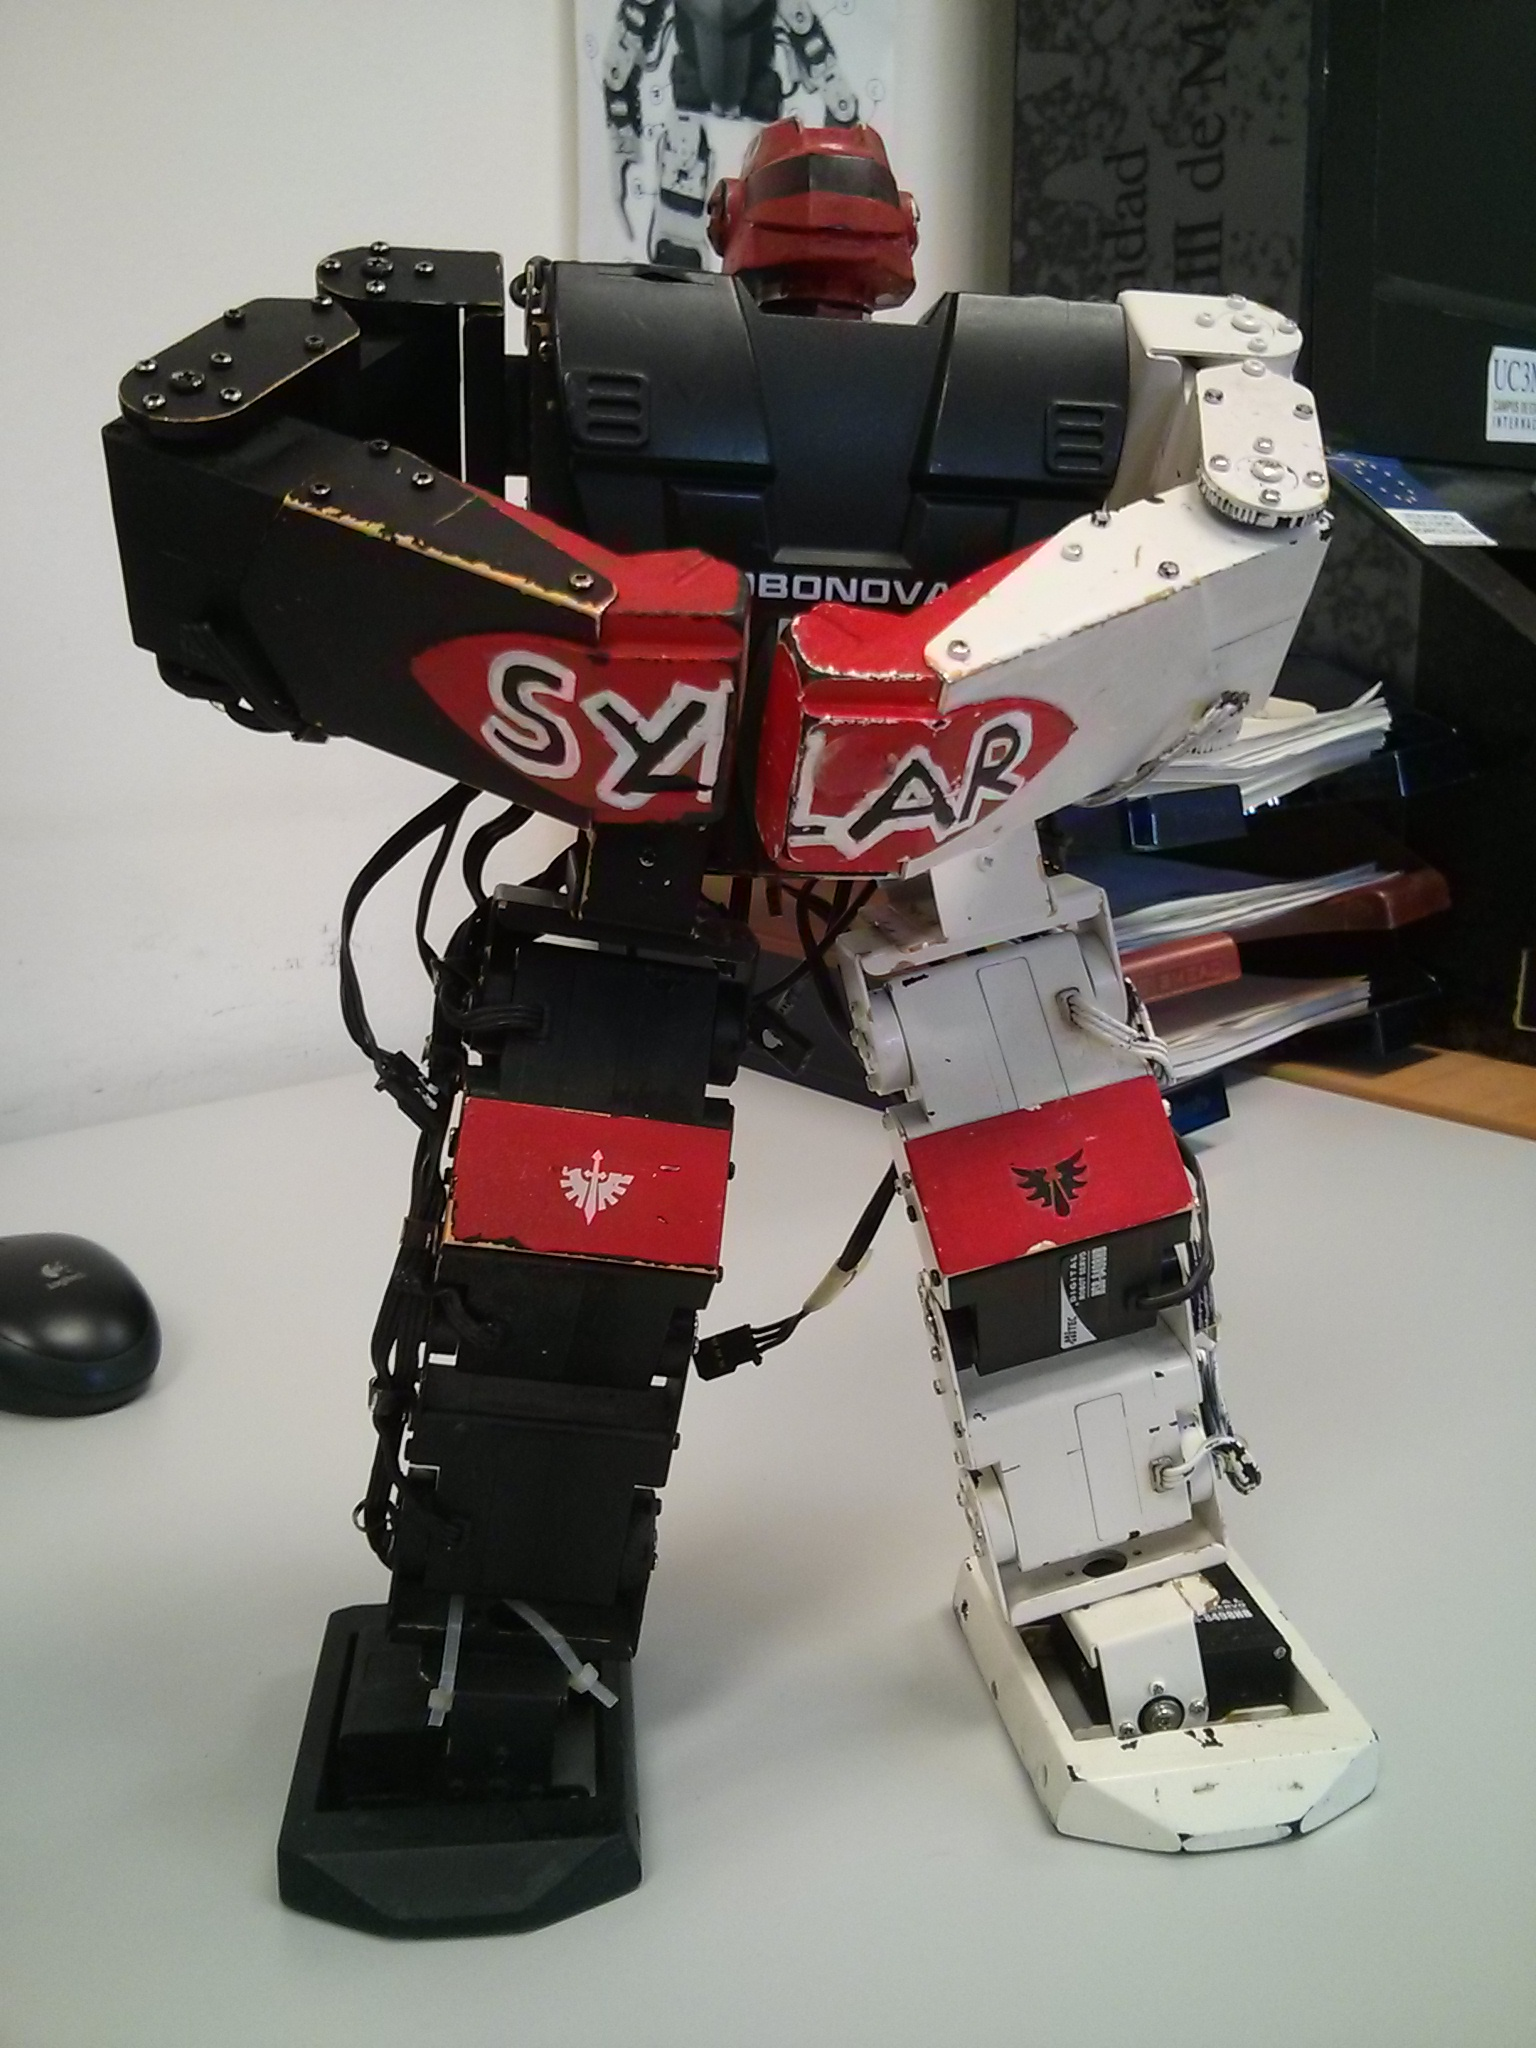
\includegraphics[width=0.45\textwidth]{figuras/sylar}   
\caption{Robot Sylar de la Asociaci�n de Rob�tica}
\label{sylar}
\end{figure}
\FloatBarrier

\medskip Por esta raz�n, desde el a�o 2013, se ha estudiado el modo de modificar estos robots con el objetivo de obtener una plataforma que permita explotar todo el potencial de sus actuadores y al mismo tiempo, facilitar la inclusi�n de nuevos componentes. Con este objetivo, se lig� fuertemente el estudio de la fabricaci�n de piezas mediante t�cnicas de impresi�n 3D con su aplicaci�n en robots mini-humanoides. Con piezas mec�nicas nuevas y electr�nicas libres, se prevee que las capacidades del robot aumenten exponencialmente. Esto convierte a los robots de la asociaci�n en una base con mucho potencial para la investigaci�n.   

\section{Campeonato CEABOT}

El campeonato nacional CEABOT re�ne cada a�o a robots mini-humanoides procedentes de universidades espa�olas y de equipos independientes. Durante tres d�as, los equipos tienen la posibilidad de presentar sus robots a diferentes pruebas de habilidad en las que pueden demostrar sus capacidades. En el reglamento de la edici�n del 2014, existen un total de cuatro pruebas combinadas de diversa tem�tica que ponen a prueba la locomoci�n, percepci�n y actuaci�n sobre el entorno de los robots participantes. Las pruebas son puntuadas por separado, sum�ndose de forma proporcional a su dificultad en la clasificaci�n final. A continuaci�n se muestran las pruebas previstas para la edici�n de 2014.

\subsection{Carrera de obst�culos}

El la carrera de obst�culos los robots deben realizar de forma aut�noma un recorrido de ida y vuelta sobre una pista de caracter�sticas fijas. En la figura \ref{carrera} se muestra el campo. �ste consiste en una superficie plana de color verde en cuya zona intermedia se colocan de forma arbitraria diferentes obst�culos inm�viles de color blanco. Estos obst�culos tienen forma paralelep�peda y unas dimensiones fijas de 20x20x50cm

\begin{figure}[h]
\centering
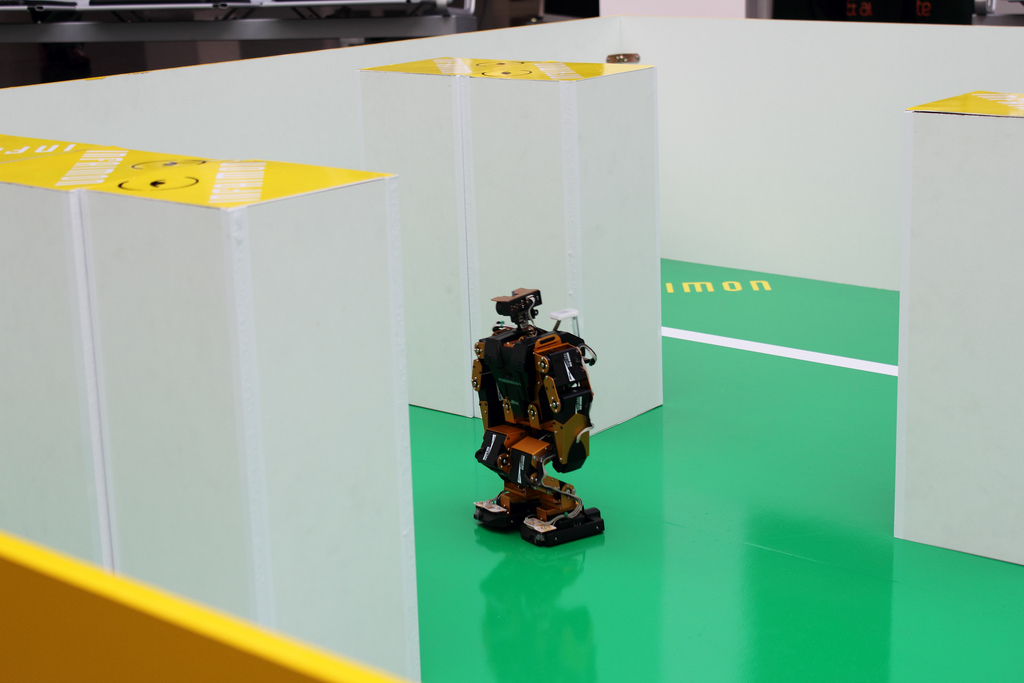
\includegraphics[width=0.7\textwidth]{figuras/carrera}   
\caption{Prueba de la carrera de obst�culos}
\label{carrera}
\end{figure}
\FloatBarrier

El robot participante debe cruzar el campo de extremo a extremo, y una vez haya accedido a la zona de llegada debe darse la vuelta y realizar el recorrido en el sentido contrario. En esta prueba se punt�a favorablemente el menor tiempo ocupado y la mayor longitud recorrida. Adem�s, las ca�das o bloqueos que requieran la intervenci�n de un juez producen penalizaci�nes en la puntuaci�n.

\subsection{Escalera}

La prueba de la escalera supone una combinaci�n de las habilidades mec�nicas y de sensorizaci�n de los robots. La prueba se desarrolla en un escenario formado por tres escalones de subida y tres escalones de bajada consecutivos. En la figura \ref{escalera} se muestra un robot mini-humanoide realizando la prueba.

\begin{figure}[h]
\centering
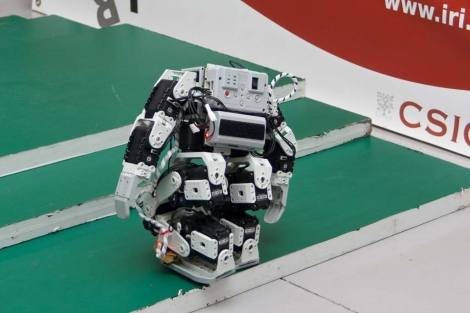
\includegraphics[width=0.6\textwidth]{figuras/escalera}   
\caption{Prueba de la escalera}
\label{escalera}
\end{figure}
\FloatBarrier

En este caso el robot debe superar escalones con una altura fija e igual a 3cm, pero con amplitud variable. El desarrollo consiste en la superaci�n de tres escalones ascendentes, cruzar la cima de las escaleras y descender otros tres escalones hasta volver al suelo. De forma similar a la prueba de navegaci�n, se punt�an el n�mero de escalones superados y el tiempo utilizado; mientras que las ca�das y bloqueos que el robot no sea capaz de manejar por s� mismo contar�n negativamente. 

\subsection{Sumo}

La prueba de sumo, que puede verse en la figura \ref{sumo}, es una de las m�s espectaculare del concurso. A diferencia del resto de pruebas, en el sumo los robots se enfrentan en parejas. Los duelos est�n constituidos por tres asaltos de dos minutos cada uno. El ring sobre el que se enfrentan los robots tiene forma circular, con un di�metro de 1.5m. Los robots compiten para derribar y/o sacar del ring a su adversario.

\begin{figure}[h]
\centering
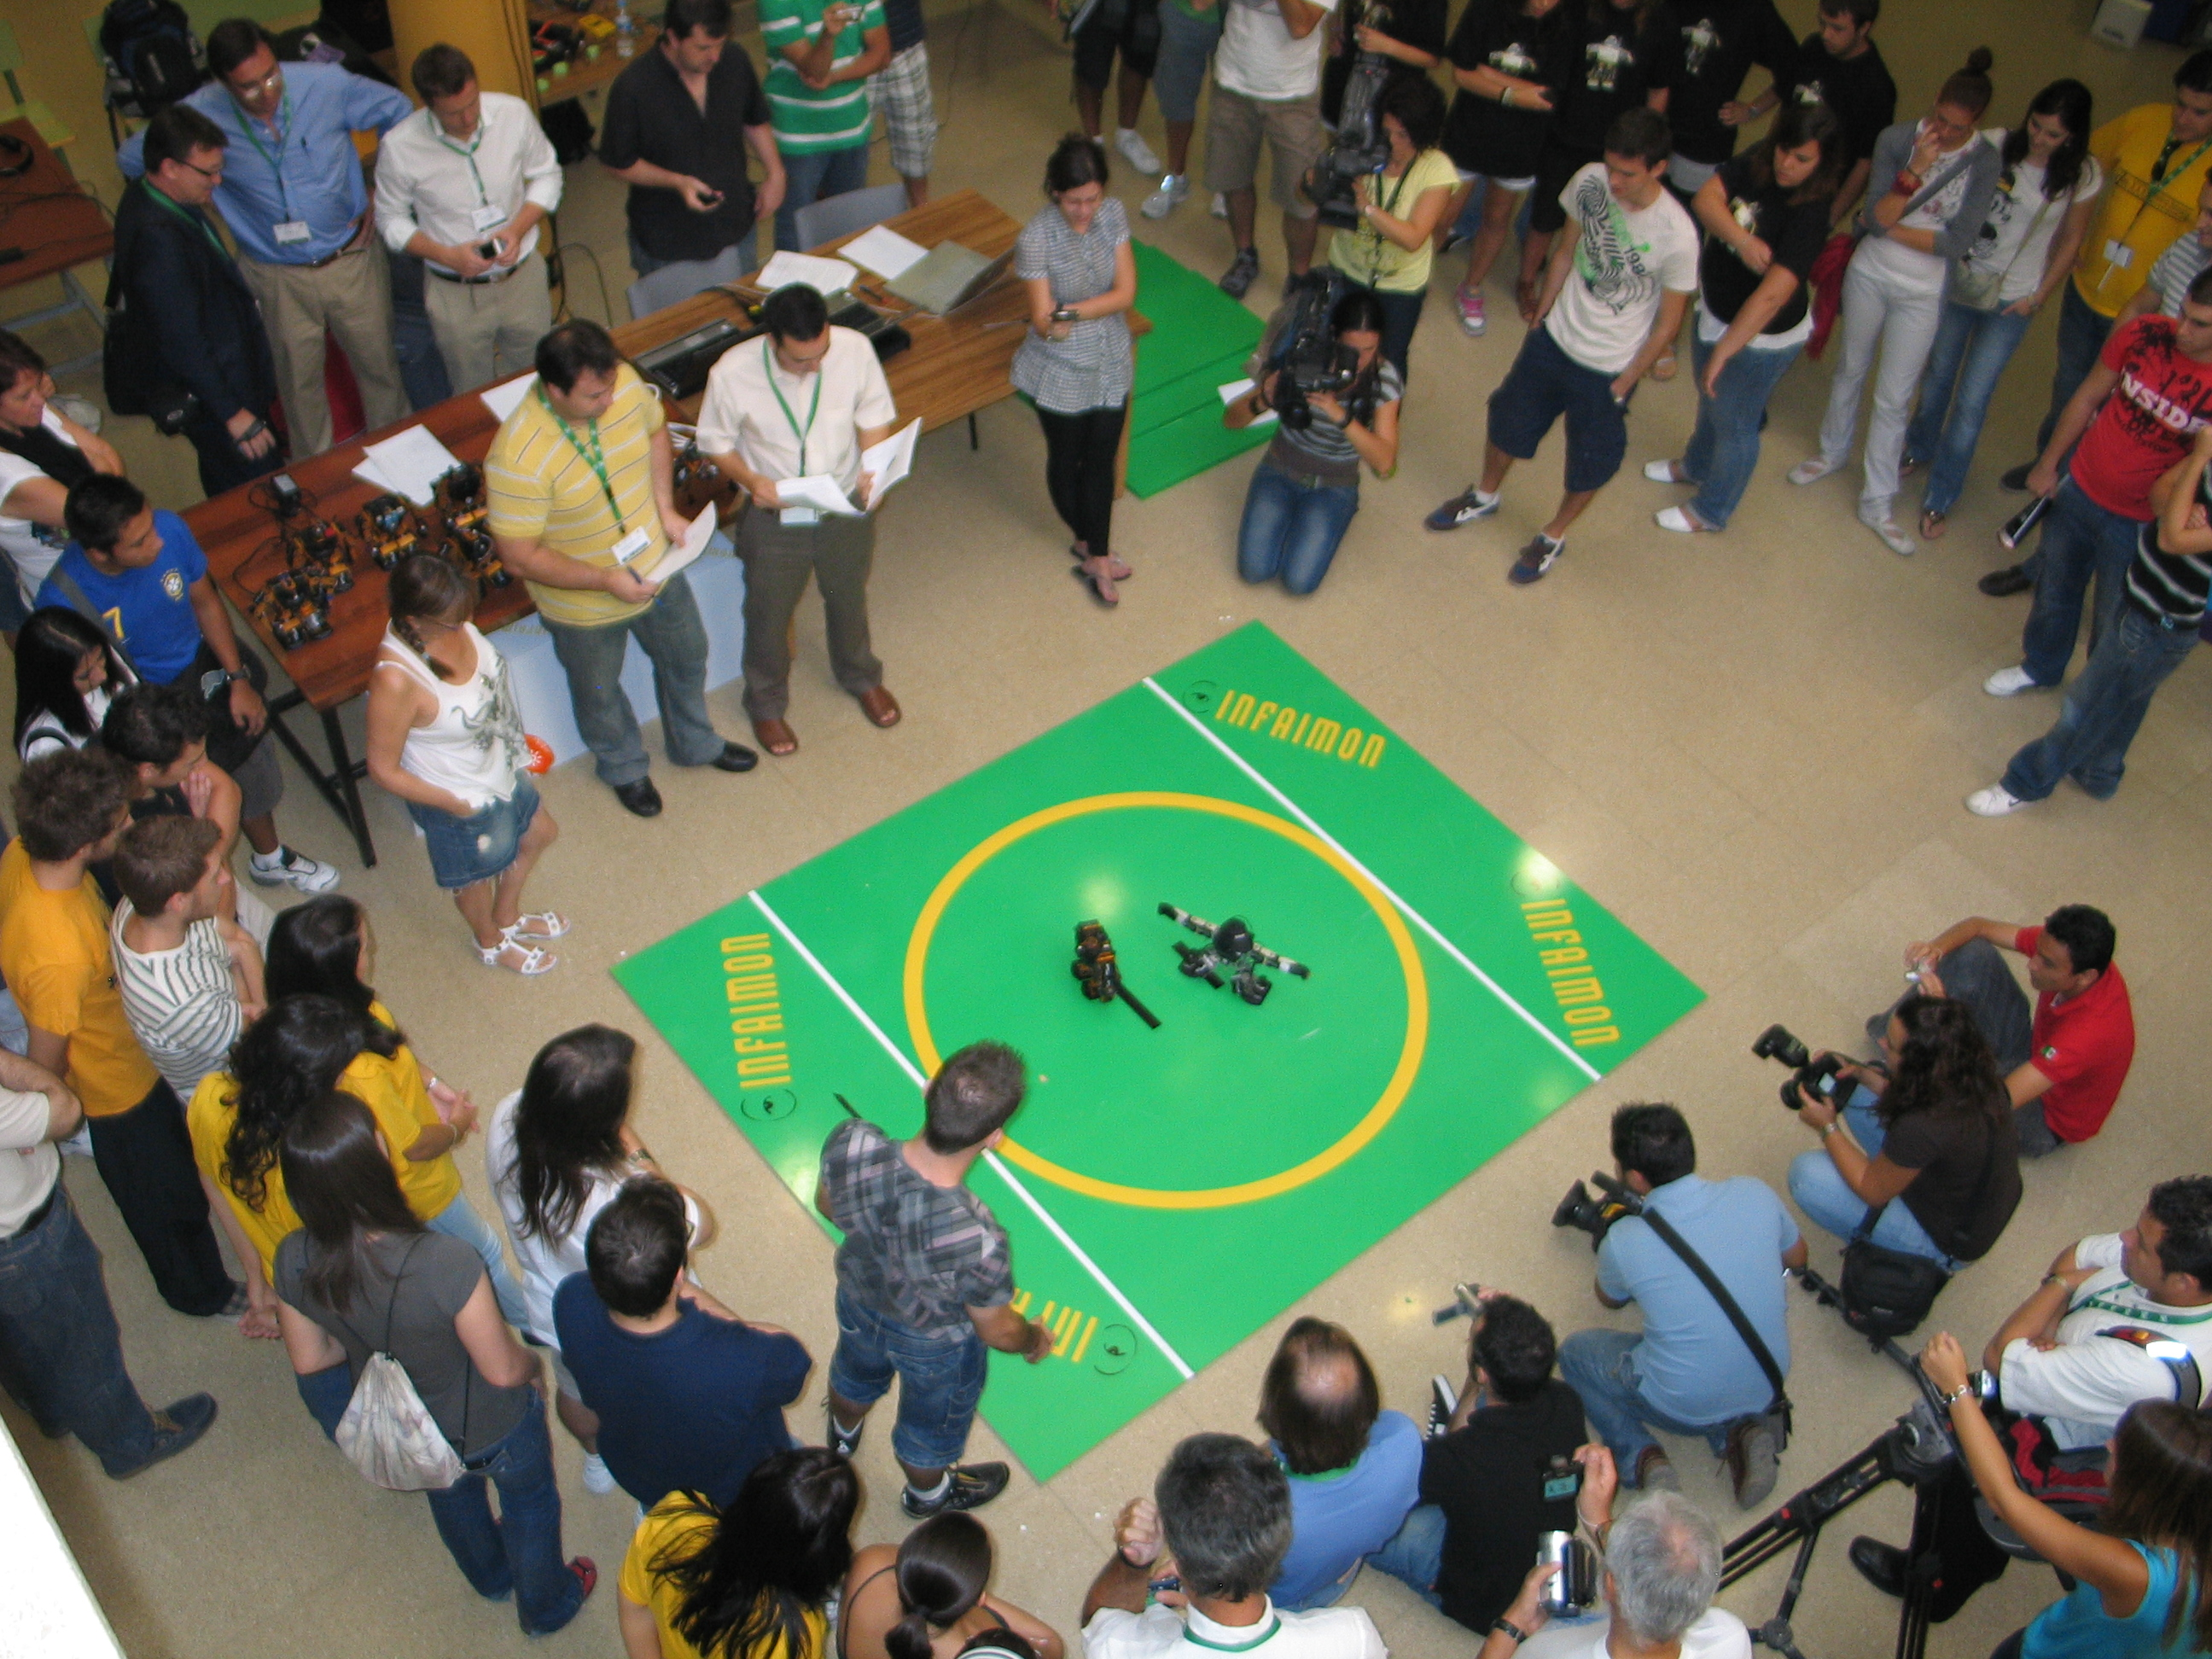
\includegraphics[width=0.65\textwidth]{figuras/sumo}   
\caption{Prueba de sumo}
\label{sumo}
\end{figure}
\FloatBarrier


\subsection{Visi�n}

La prueba de visi�n se presenta como una novedad en la edici�n de 2014 del concurso. Por primera vez se implanta en la competici�n una prueba que obliga a los robots a portar una c�mara y realizar procesamiento de im�genes para su superaci�n. El tablero de juego se comparte con el campo de la carrera de obt�culos. En esta prueba, el robot se colocar� en el centro del tablero, y a su alrededor se colocar�n obstaculos (los mismos que en la carrera de obst�culos) en intervalos de 45�. En la parte superior de los obst�culos se colocar� un rectangulo rojo con un c�digo QR en su interior, tal y como se indica en la figura \ref{pruebavision}. El robot deber� leer el c�digo QR, en el que se le indicar� una rotaci�n que le permitir� encontrar el siguiente marcador. De esta forma, el robot deber� seguir una secuencia de rotaciones para superar la prueba.

\begin{figure}[h]
\centering
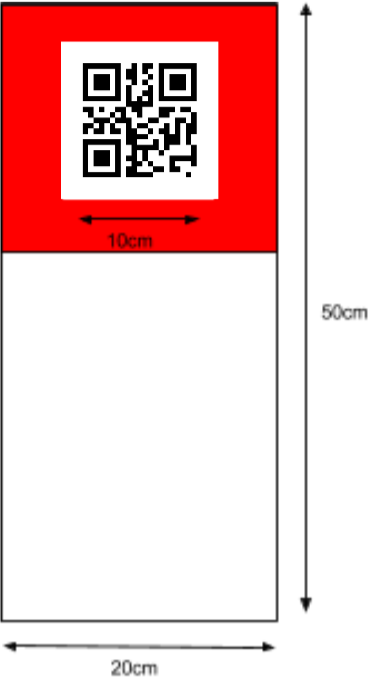
\includegraphics[width=0.45\textwidth]{figuras/pruebavision}   
\caption{Marcador de la prueba de visi�n}
\label{pruebavision}
\end{figure}
\FloatBarrier





\chapter{Estado del arte}



\section{Plataformas rob�ticas mini-humanoides}

Robots 



\section{Competiciones}
\subsection{RoboGames}

Robots estructuralmente molones multidisciplinares


\subsection{Robo-One}

Robots estructuralmente molones, fuertes, estables, radiocontrolados. Compiten cara a cara muchos equipos

\subsection{Robocup}

Enjambres, vision, proramaci�n coordinada. Entornos din�micamente VARIABLES.

\subsection{Ceabot}

Robots individuales, compiten solos en entornos "complejos" pero FIJOS

\section{Locomoci�n}
hablar del motion, del pypose... contra un zmp y cosas asi



\section{Visi�n}




%%chapter introduce un nuevo cap�tulo

\chapter{Objetivos TODO ESQUEMATIZADO }

%gmmgfngfngfngfngfngfnhgf
%\begin{itemize}
%\item \textbf{ejemplo de lista de puntos}.

%Cocoloco loco loco loco tacacacaca
%\item \textbf{ejemplo de lista de puntos}.\\Cocoloco loco loco loco %tacacacaca
%\item \textbf{ejemplo2 de lista}.
%\end{itemize}

\section{Desarrollar una plataforma rob�tica humanoide}

TODO El primer objetivo de este proyecto es el desarrollo de una plataforma rob�tica humanoide de prop�sito general. Para llegar a ello ser� necesario estudiar los componentes que forman un robot humanoide Sus capacidades deben ser al menos suficientes para desarrolar sobre la plataforma los objetivos del segundo punto.

- Que la plataforma sea lo suficientemente cojonuda para poder hacer esto y mas 

\subsection{Estudiar los componentes que necesita un robot humanoide}

- Se realizar� un estudio de elementos necesarios para un robot
- Se evaluar� cuales funcionan mejor y peor
- Se analizar� cuales son dignos de meterse en mi robot
- Se escoger� una configuraci�n completa 

\subsection{Integrar una c�mara USB}

- Se requiere integrar una c�mara para hacer algoritmos de visi�n
- Se requiere que la c�mara entre integrada f�sicamente en el robot.
- Que la c�mara pueda moverse en el robot.

\subsection{Integrar un controlador}

- Un controlador que permita mover el robot y procesar visi�n.
- Que pueda programarse libremente sin casarse con Robotis.
- Que permita a�adir sensores y actuadores libremente.
- Que se integre fisicamente dentro del robot.
- Que funcione (capacidades de procesamiento, autonom�a... etc)


\subsection{Realizar las modificaciones esctructurales que sean pertinentes}

- Dise�ar piezas que requiera el robot (para montar sensores, c�mara...)
- Dise�ar piezas que no se requieran pero mejoren el comportamiento
- Dise�arlas para que puedan imprimirse con una impresora 3d.
- Imprimirlas todas

\section{Puesta en marcha y programaci�n}

El robot debe ponerse en marcha y funcionar, desde su montaje hasta su participaci�n en CEABOT

\subsection{Desarrollar locomoci�n}

- Controlar movimientos de las articulaciones
- Programar movimientos complejos
- Hacer que ande
Hacer el control de movimientos desde el movimiento de un servo has el movimiento de extremidades y con ello 

\subsection{Desarrollar algoritmos de visi�n}

- Hacer algoritmos de visi�n con OpenCV
- Que funcionen dentro del robot
- Optimizados para funcionar en condiciones



\subsection{Desarrollar aplicaciones de competici�n}

- Apoyandose en vision
- Con los movimientos creados
- Integrando la informaci�n de sensores
- Consiguiendo pasar las pruebas

sando de base las dos cosas anteriores el robot tiene que poder funcionar los suficientemente bien como para hacer programillas para las pruebas concretas.





\paragraph{Palabras clave:} TODO palabraclave1, palabraclave2, palabraclave3.


%chapter introduce un nuevo cap�tulo
\chapter{Elecci�n de componentes}

Como punto de partida, se han seleccionado una serie de componentes adecuados para dotar al robot con las capacidades necesarias para cumplir los objetivos.

\section{Plataforma rob�tica}

El primer paso para la realizaci�n de este proyecto fue el estudio y selecci�n de las plataformas rob�ticas que pueden conseguirse actualmente. Dado que el objetivo es encontrar un robot humanoide sobre el que se pueda implantar un sistema de visi�n, es necesario analizar diversos aspectos; algunos mec�nicos como el numero y fuerza de los actuadores, y otros electr�nicos como la capacidad de procesamiento y velocidad del controlador. Sin embargo, dado que este proyecto es autofinanciado en su mayor medida, el factor econ�mico tambi�n es un limitante destacable. Buscamos una plataforma que cumpliese los siguientes requisitos:

\begin{itemize}
\item \textbf{Programable en C/C++} 

Se requiere que sea programable en C/C++ y que adem�s no dependa de una IDE concreta.

\item \textbf{Posibilidad de conectarle una c�mara}

Se necesita que permita conectarle una c�mara y realizar programas con OpenCV.

\item \textbf{Expandible con sensores y actuadores}

El sistema debe permitir la adici�n de nuevos sensores y actuadores, sin verse limitado por hardware o software.

\item \textbf{Servos de al menos 12kg/cm}

Ya que se van a incluir nuevas partes, es absolutamente necesario que los servos puedan soportar carga adicional colocada en el robot.

\item \textbf{Chasis reconfigurable}

Aunque no es tan importante como el resto, es posible que el robot requiera modificaciones, por lo que una base reconfigurable y vers�til ser� apreciada.

\end{itemize}

En el siguiente apartado se presenta un estudio las principales opciones.

\subsection{Selecci�n de una plataforma rob�tica}

En el mercado existe una gran variedad de robots educativos que cumplen las caracter�sticas antropom�rficas necesarias para ser considerados robots mini-humanoides. Los robots que se muestran a continuaci�n son una recopilaci�n de algunos de los modelos mas accesibles y extendidos.

\subsubsection{Hitec Robonova}

El Robonova (figura \ref{robonova}) es uno de los mini-humanoides mas extendidos a nivel mundial. Fue uno de los primeros robots de este tipo que se fabric� comercialmente y marc� un antes y un despues en su categor�a. Es por esto que es muy com�n encontrar Robonovas en competiciones como Ceabot, ya que durante muchos a�os fue el robot mini-humanoide mejor equipado y mas vendido. En la Asociaci�n de Rob�tica de la Universidad Carlos III, se han utilizado Robonovas en competiciones y proyectos desde su fundaci�n.

\begin{figure}[h]
\centering
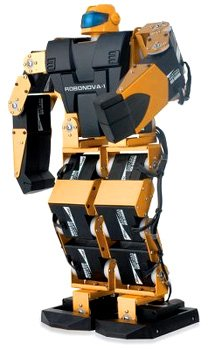
\includegraphics[width=0.4\textwidth]{figuras/robonova}   
\caption{Hitec Robonova}
\label{robonova}
\end{figure}

El kit de f�brica cuenta con 16 grados de libertad. Sus actuadores son servos digitales HSR 8498HB, que desarrollan un torque de 7.4kg/cm. Cabe destacar de estor servos su funci�n "Motion Feedback", es decir, su capacidad para leer posiciones y comunicarselas al controlador.
La placa de control del Robonova est� basada en un microcontrolador ATMega 128 y cuenta con hasta 40 pines GPIO (puertos binarios de entrada y salida), 8 entradas anal�gicas, 3 salidas PWM, puerto serie y conexi�n I2C. Gracias a esto, el Robonova es f�cilmente ampliable con sensores y actuadores, no necesariamente de la misma marca. En cuanto al software, Hitec da soporte a la programaci�n con RoboBasic, un entorno de desarrollo completo con un lenguaje basado en Basic. 

\subsubsection{Kondo KHR-3HV}

El KHR-3HV (figura \ref{kondo}), del fabricante japon�s Kondo, es uno de los mini-humanoides mas avanzados actualmente. Puede presumir de ser el modelo de serie mas utilizado en el campeonato Robo-One, siendo seleccionado por los equipos por su gran agilidad y tama�o compacto.

\begin{figure}[h]
\centering
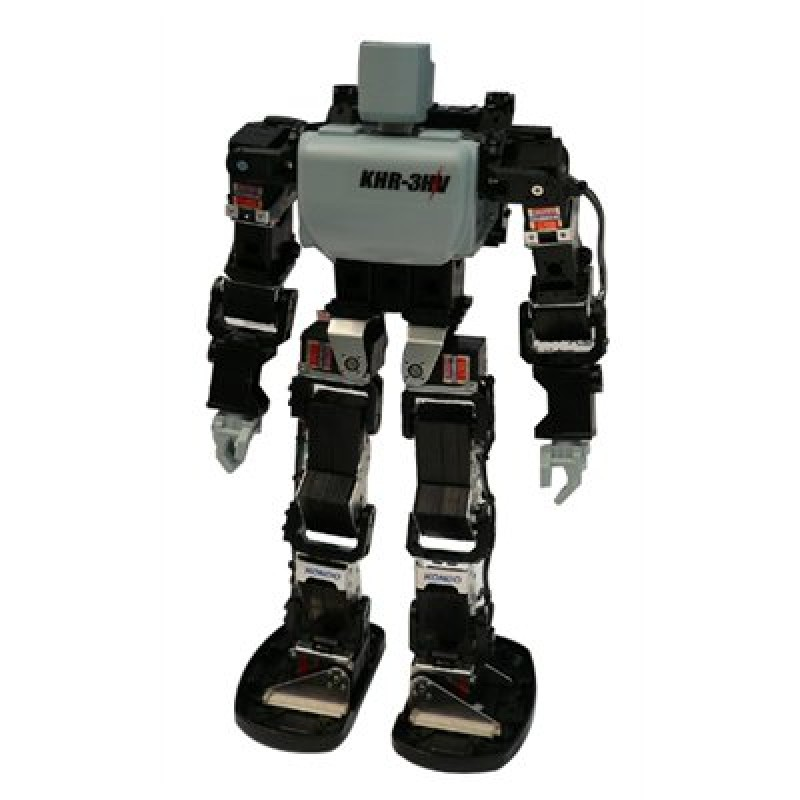
\includegraphics[width=0.8\textwidth]{figuras/kondo}   
\caption{Kondo KHR-3HV}
\label{kondo}
\end{figure}

En su configuraci�n standard, el KHR-3HV cuenta con 17 servomotores KRS-2552HV de 14kg/cm de torque. Dichos actuadores, adem�s, incluyen un peque�o microcontrolador, lo que les permite conectarse en daisy chain. El robot incluye una controladora RCB-4, expandible con 10 entradas analogicas y 10 GPIOs, y con capacidad para controlar hasta 35 servos. El software de programaci�n ofrecido por Kondo es el Heart to Heart V4, que puede ser descargado gratuitamente desde su web oficial. Es importante recalcar que gracias a su inmensa comunidad de usuarios, existen varios proyectos de c�digo abierto con librer�as que permiten programar el KHR-3HV en lenguajes mas convencionales, como C y Python.


\subsubsection{Vstone Robovie-X}

El Robovie-X, uno de los robots humanoides de la empresa Vstone, se presenta en tres versiones diferentes: Lite, Standard y PRO. La diferencia entre los tres modelos radica en el n�mero y tipo de servos que montan, manteniendo comunes el resto de partes del robot. El modelo Standard (figura \ref{robovie}) posee 17 grados de libertad, movidos por servos VS-S092J que desarrollan un torque de 9.2kg/cm. El controlador es un VS-C1, el cual tiene 30 canales para controlar servos. Vstone tambi�n fabrica diversas placas de expansi�n para la conexi�n de sensores en el Robovie-X.

\begin{figure}[h]
\centering
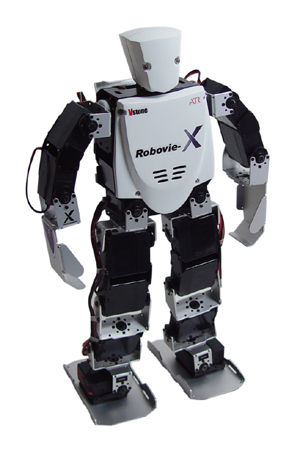
\includegraphics[width=0.5\textwidth]{figuras/robovie.jpg}
\caption{Vstone Robovie-X}
\label{robovie}
\end{figure}

Junto al robot se suministra el programa RobovieMaker2, necesario para programarlo. El m�todo de programaci�n est� orientado a la construcci�n de diagramas de flujo desde los que se controlan tanto los movimientos como la lectura de sensores externos.


\subsubsection{Robotis Bioloid}

La empresa koreana Robotis, comercializa un kit rob�tico conocido como Bioloid. Este kit proporciona una amplia gama de piezas diferentes para montar distintos modelos de robots. La modularidad de los componentes le convierten en una base excelente sobre la que realizar modificaciones, pudiendo dise�ar configuraciones alternativas con gran facilidad.

El robot Bioloid (figura \ref{bioloid}) incluye 18 servos Dynamixel, modelo AX-12A o AX-18A, dependiendo de la versi�n del kit. Los actuadores Dynamixel est�n controlados internamente por un microcontrolador ATMega8. Gracias a �l, estos servos permiten realizar funciones avanzadas tales como el control de velocidad, torque, temperatura de ejecuci�n... etc, posibilitando procesar informaci�n de bajo nivel directamente dentro del actuador y pudiendo abstraer el control de la controladora del robot a un nivel superior.

En cuanto a su controladora, los kits proporcionan controladoras de Robotis de la serie CM, mas espec�ficamente, la CM-5 en el caso del Bioloid Comprehensive y la CM-510 o CM-530 (seg�n qu� versi�n) en el Bioloid Premium y GP.


\begin{figure}[h]
\centering
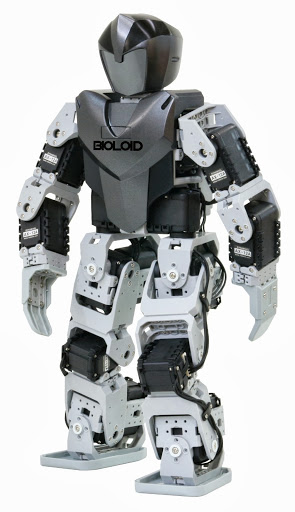
\includegraphics[width=0.4\textwidth]{figuras/bioloid.JPG}   
\caption{Bioloid Premium}
\label{bioloid}
\end{figure}


\begin{itemize}
\item \textbf{Robotis CM-5}.

Cuenta con un microcontrolador ATMega128. Permite la conexi�n de sensores espec�ficos de la marca en el bus TTL, como el Dynamixel AX-S1.
\item \textbf{Robotis CM-510}.

Basada en un microcontrolador  ATMega2561. Adem�s de los sensores de la propia marca (Dynamixel AX-S1, gir�scopo...), que pueden montarse conectados al bus TTL, tiene cinco puertos para la conexi�n de sensores de salida anal�gica. Adicionalmente, posee un puerto para conectar un receptor ZigBee y teleoperar el robot.
\item \textbf{Robotis CM-530}.
 
Presentado como la evoluci�n de la CM-510, en este caso el microcontrolador de la placa es un ARM Cortex STM32F103RE, de 32 bits. El resto de caracter�sticas son similares a las de la CM-510, tiene cinco puertos de expasi�n para sensores anal�gicos y un puerto para conectar un receptor ZigBee o Bluetooth.
\end{itemize}

En cuanto a la programaci�n, Roboplus ( TODO foto ) es una suite de programas distribuida gratuitamente por Robotis para la programaci�n de sus robots educativos. Destaca por ser un entorno con un lenguaje de programaci�n (R+) muy visual e intuitivo, preparado para su uso por ni�os o gente sin conocimientos muy avanzados de programaci�n. Sin embargo, esto lo convierte en un lenguaje de programaci�n muy limitado, hasta el punto que no permite utilizar todo el potencial de los actuadores Dynamixel.



\subsubsection{comparativa y elecci�n final TODO}

Realizando un primer an�lisis, ninguno de los robots candidatos cumple los requ�sitos. Todos utilizan IDEs y lenguajes propios para su programaci�n. El Robonova y el Robovie tienen unos servos demasiado d�biles, lo que dificultar�a mucho a�adir mas peso al robot. En lo que a grados de libertad se refiere, solo el Bioloid es capaz de rotar las pierna en un eje perpendicular al suelo, lo que supone una ventaja a la hora de programar la locomoci�n del robot. Entre el Kondo y el Bioloid, se ha elegido el Bioloid por tres razones: Es mas f�cil de modificar, el kit trae mas servos, y es mas barato.


\section{Modificaciones estructurales}

El Bioloid Comprehensive es un buen punto de partida, sin embargo tiene algunos puntos d�biles que conviene revisar. Adem�s, para poder implantar en el robot los dispositivos que requiere este proyecto se necesitar� mejorar las capacidades de la plataforma.

\subsection{Cabeza m�vil TODO}

Un requisito importante del proyecto es permitir que la c�mara que vamos a montar pueda moverse con libertad para enfocar a diferentes zonas de su entorno. Dado que en CEABOT la mayor�a de los datos  que aporta el entorno est�n situados en el suelo, necesitamos que la c�mara al menos pueda dirigirse hacia el frente y hacia el suelo. Esto lo conseguiremos con la adici�n de un microservo PWM y una plataforma articulada para la cabeza. Dadas las caracter�sticas de este movimiento, no necesitamos un servo con grandes capacidades, ya que su rango de acci�n estar� muy limitado y su efecto ser� despreciable en el reparto de pesos del robot.

[FOTO REAL DEL MICROSERVO]

Se ha elegido un microservo PWM por su bajo tama�o y peso, su bajo precio y su sencillez a la hora de montarlo y programarlo. El principio de funcionamiento de un servo PWM es muy simple. De las tres patillas de su conector, dos son de alimentaci�n y la tercera se encarga de recibir una onda PWM que, variando la amplitud de su pulso, ordena al servo a colocarse en la posici�n fijada.

Particularmente, se ha escogido un servo Tower Pro MG90s (figura \ref{microservo}) cuyas especificaciones presentan un torque de 2.4=kg/cm, y una transmisi�n met�lica soportada por rodamientos. Este �ltimo dato es muy importande si tenemos en cuenta que el sistema de cabeza m�vil se situar� en una zona extrema del robot, y que un golpe producido por una caida forzar� de forma directa el eje del servo de la articulaci�n. Este servo proporcionar� a la cabeza la robustez necesaria para salir indemne de este tipo de accidentes, muy comunes teniendo en cuenta que el robot estar� destinado a la realizaci�n de pruebas de competici�n.

\subsection{Cintura m�vil TODO}

Otra de las modificaciones b�sicas a realizar sobre la paltaforma rob�tica, ha sido la inclusi�n de un servo adicional Dynamixel AX-12A para articular la cintura. A parte de la mejora de capacidades que se produce en los movimientos del robot, servir� para girar la direcci�n de la c�mara radialmente. Podr�a decirse que entre el servo de la cabeza y el de la cintura, se ha creado un sistema distribuido de pan-tilt ( TODO explicar qu� significa ) que permitir� mover la c�mara en todas las direcciones manteniendo fija la base del robot, es decir, sus piernas.

\section{Sensorizaci�n TODO}

El funcionamiento del robot y su control va a estar basado principalmente en la c�mara y los algoritmos de visi�n que se programar�n. No obstante, la c�mara consume muchos recursos del procesador y existen alguna tareas sencillas que es mas f�cil programar con sensores mas simples. A continuaci�n se muestra un estudio de sensores que pueden ser �tiles en el proyecto.

\subsection{Sensores de distancia TODO}

Existen diferentes tipo de sensores de distancia. El prop�sito de estos sensores no es otro que la medici�n de longitudes f�sicas utilizando diferentes principios f�sicos. Se ha planteado el uso de sensores infrarrojos y de sensores de ultrasonidos.

\subsubsection{Sensores de infrarrojos TODO}

Los sensores de infrarrojos basan su funcionamiento en la reflexi�n de luz infrarroja sobre superficies. El sensor est� formado por dos LEDs infrarrojos, uno emisor y otro receptor. El emisor emite de forma continua una luz infrarroja dirigida hacia un punto fijo. Si en ese punto fijo se encuentra un objeto f�sico, la luz se reflejar� y ser� captada por el diodo receptor. La salida de estos sensores se mide mediante la diferencia de potencial que se produce en el diodo receptor. Se ha estudiado la inclusi�n en el proyecto de sensores infrarrojos Sharp, especialmente de su modelo GP2Y0A21YK, que tiene un rango de operaci�n de entre 4 y 150cm. En la gr�fica de la figura \ref{graficair} se presenta la variaci�n de tensi�n de salida respecto a distancia para un Sharp GP2Y0A21YK.

\begin{figure}[H]
\centering
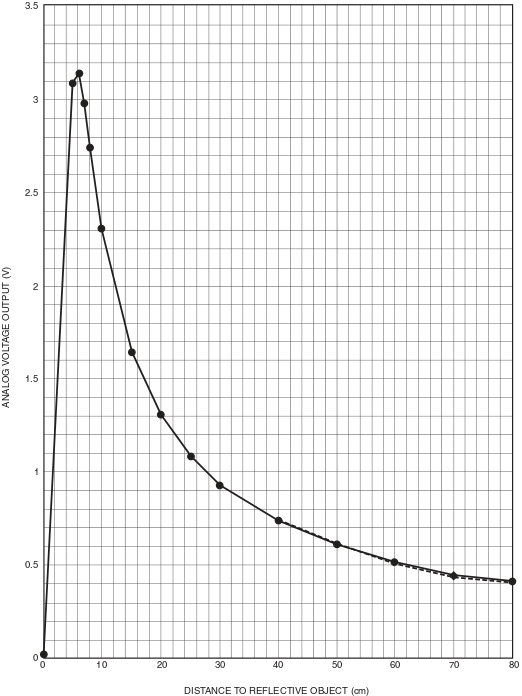
\includegraphics[width=0.8\textwidth]{figuras/graficair}   
\caption{Salida de un sensor Sharp respecto a su medici�n.}
\label{graficair}
\end{figure}

\subsubsection{Sensores de ultrasonidos TODO}

Los sensores de ultrasonidos detectan distancias basandose en el tiempo en el que un ultrasonido recorre el espacio. Normalmente, los sensores de ultrasonidos tienen dos focos, uno emisor y otro receptor. Una de las diferencias de este tipo de sensores con los sensores infrarrojos es que mientras los sensores infrarrojos toman medidas de un punto, el rango de operaci�n de los sensores de ultrasonidos se abre en un como de 60� de amplitus desde su emisor. Se ha analizado el sensor de ultrasonidos HC-SR04 como posible candidato para formar parte del robot por su f�cil accesibilidad. Otro punto importante es que en estos sensores la salida es proporcional a la distancia medida, es decir, se adec�a a una recta. Es por esto por lo que podremos realizar medidas reales directamente midiendo la salida del sensor.

\subsubsection{Experimentos de medida TODO}


\begin{figure}[H]
\centering
\begin{tabular}{ >{\centering\arraybackslash}m{0.5\textwidth} >{\arraybackslash}m{0.5\textwidth}}
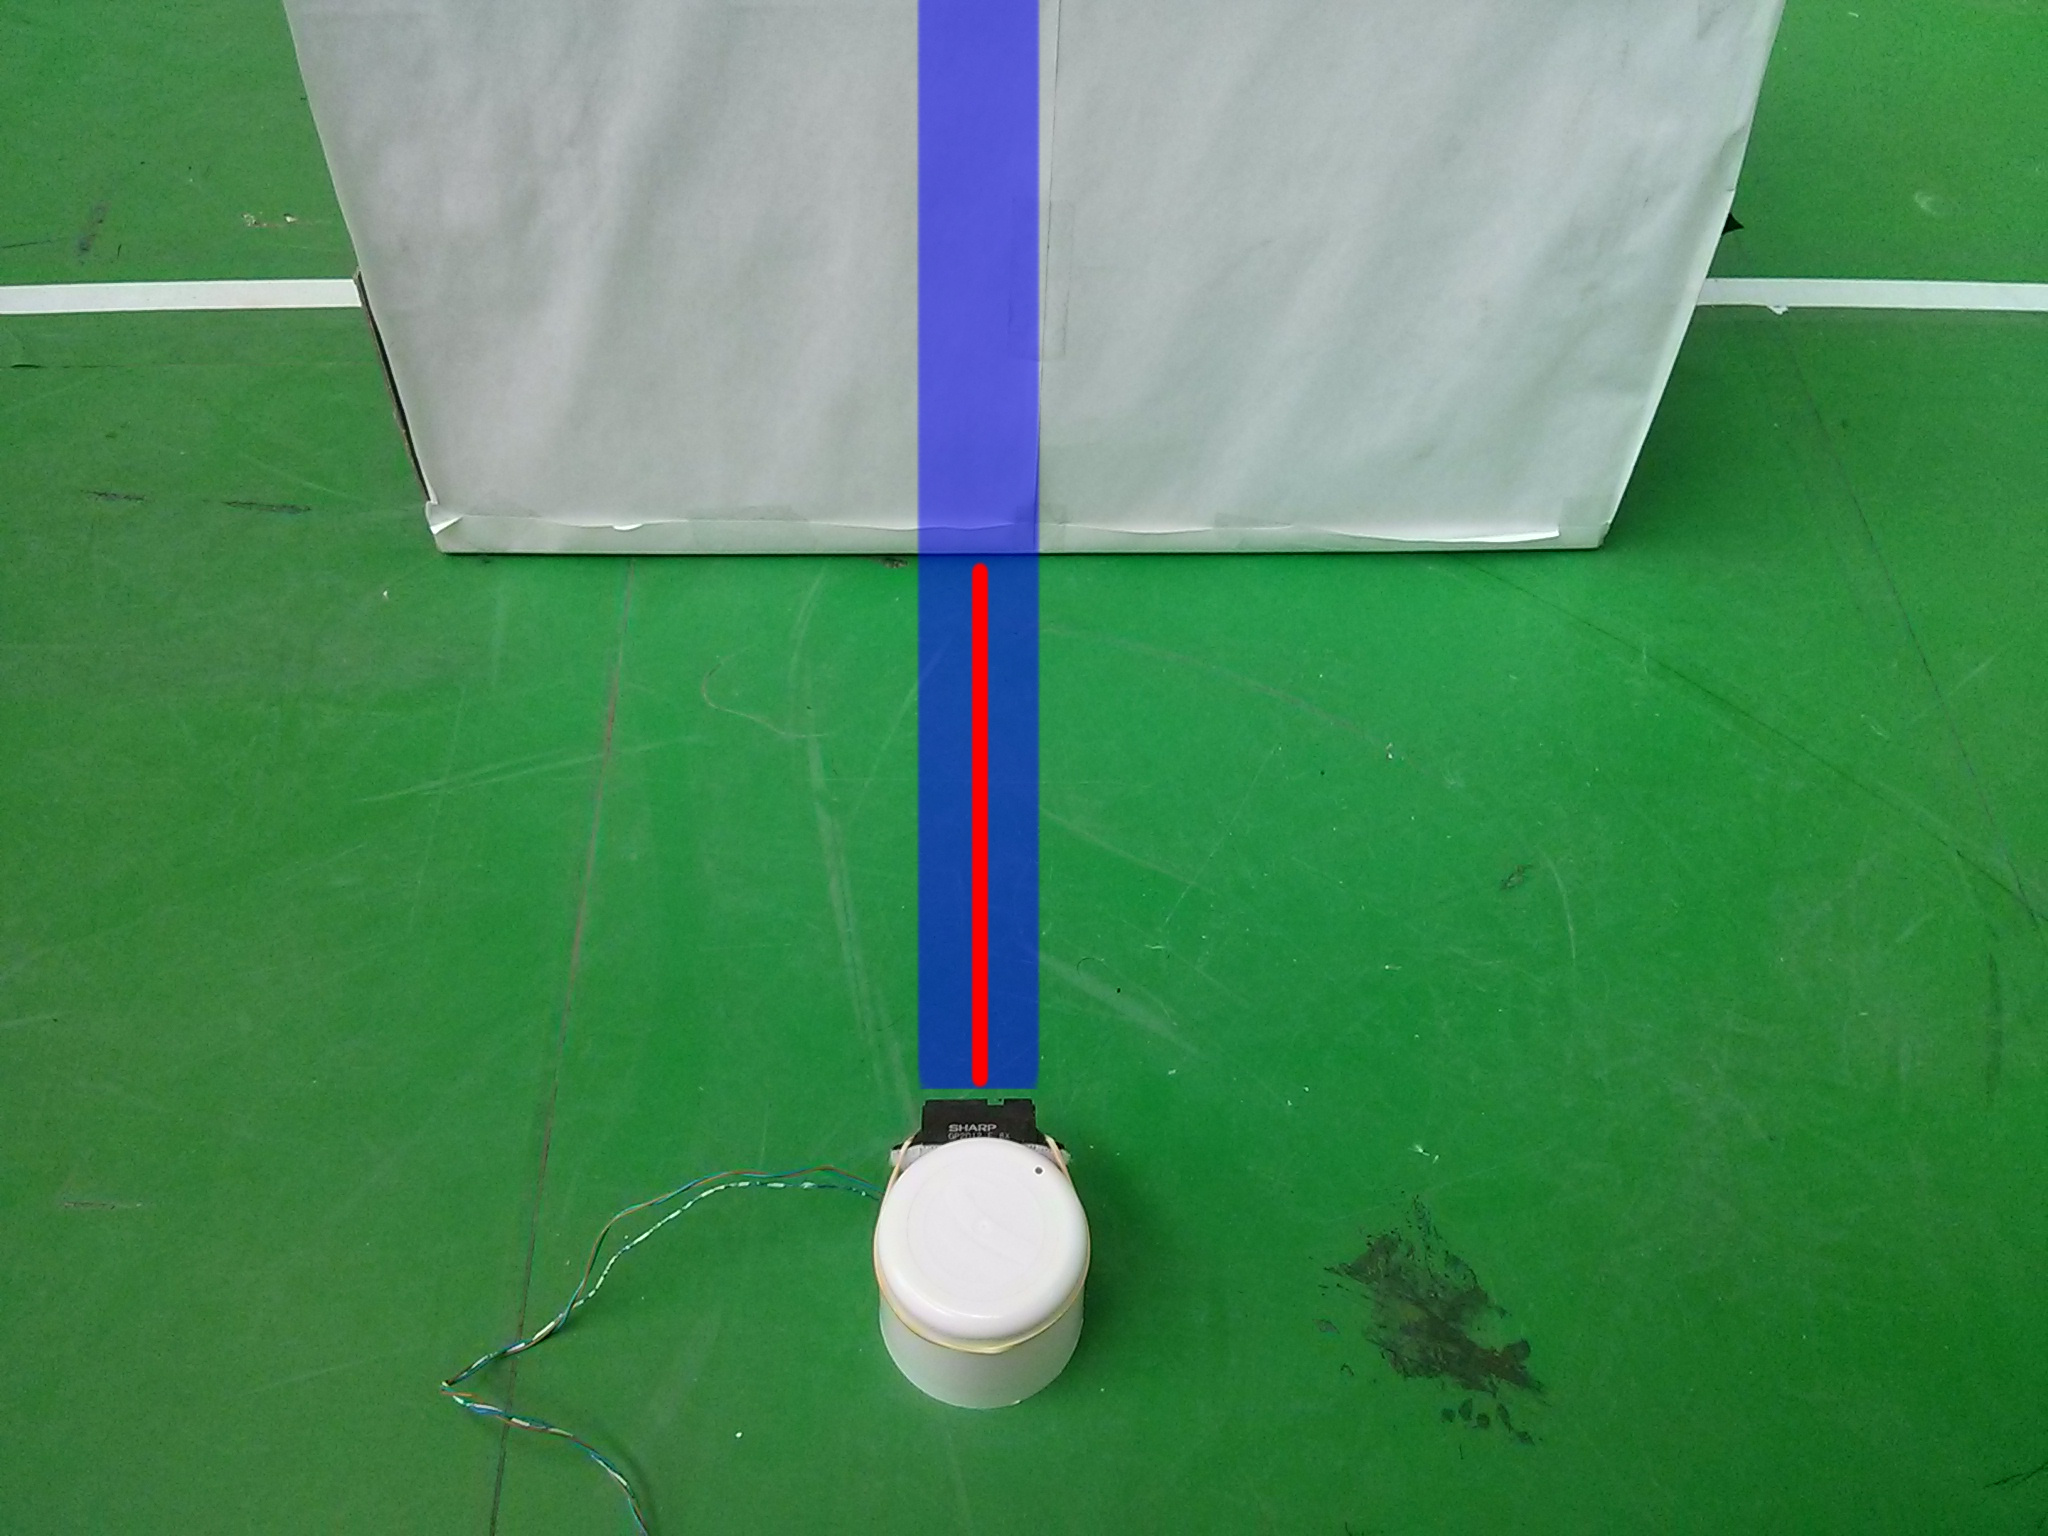
\includegraphics[width=0.5\textwidth]{figuras/expir1} & 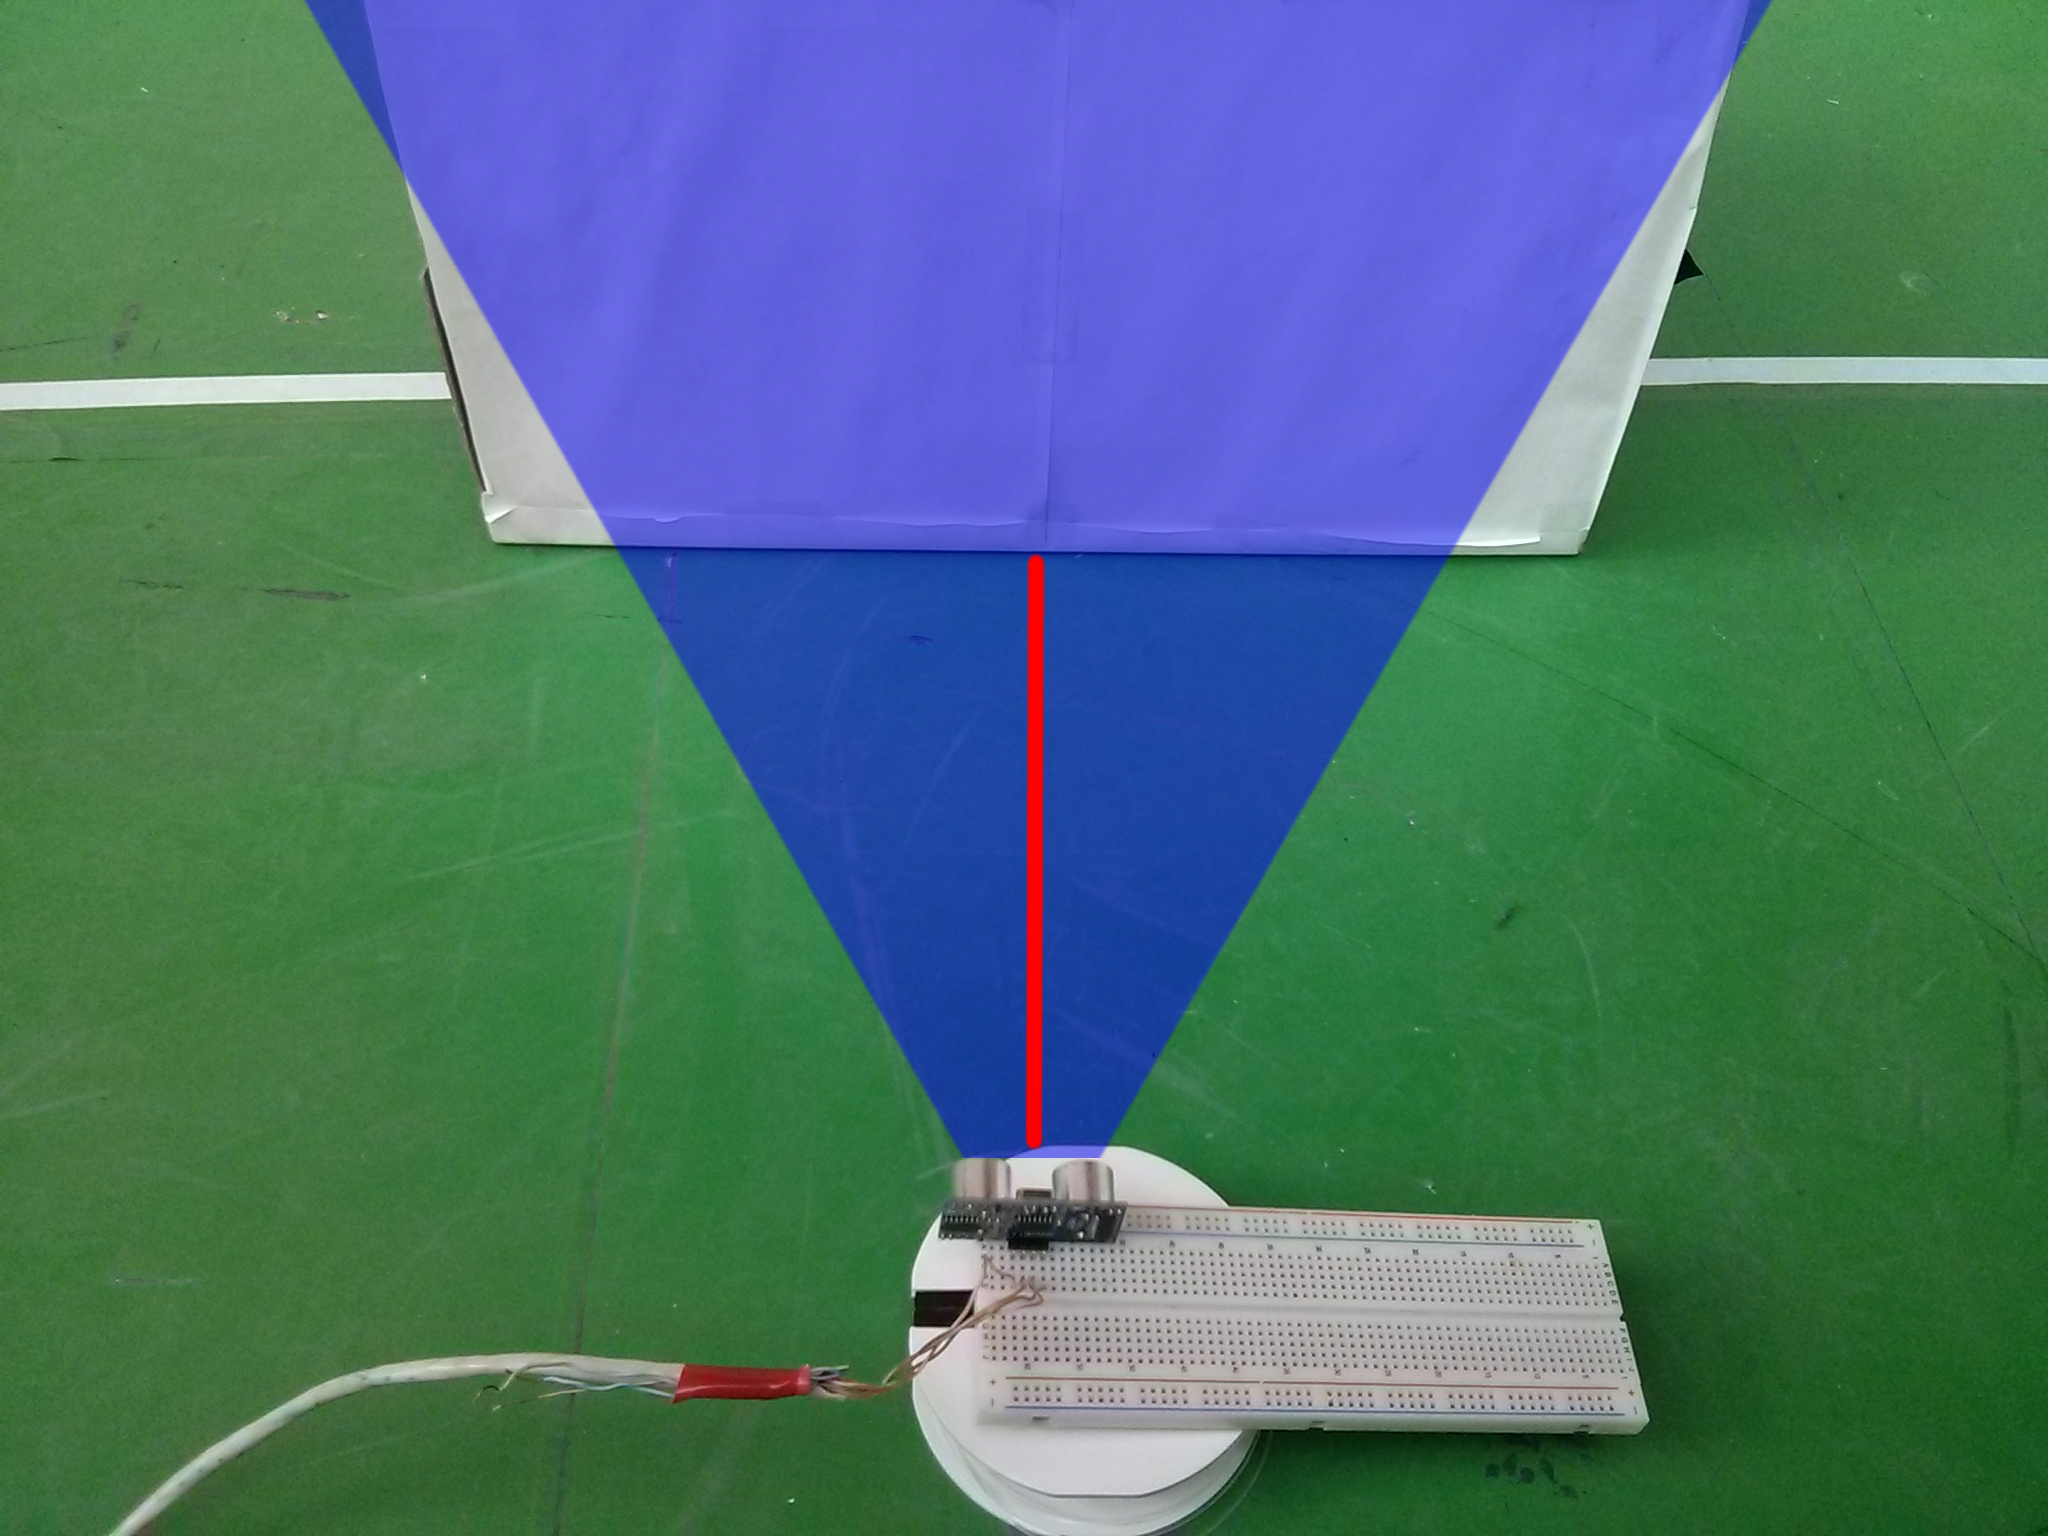
\includegraphics[width=0.5\textwidth]{figuras/expus1}  \\
\end{tabular}
\caption{Primer experimento.}
\label{experimento1}
\end{figure} 

\begin{figure}[H]
\centering
\begin{tabular}{ >{\centering\arraybackslash}m{0.5\textwidth} >{\arraybackslash}m{0.5\textwidth}}
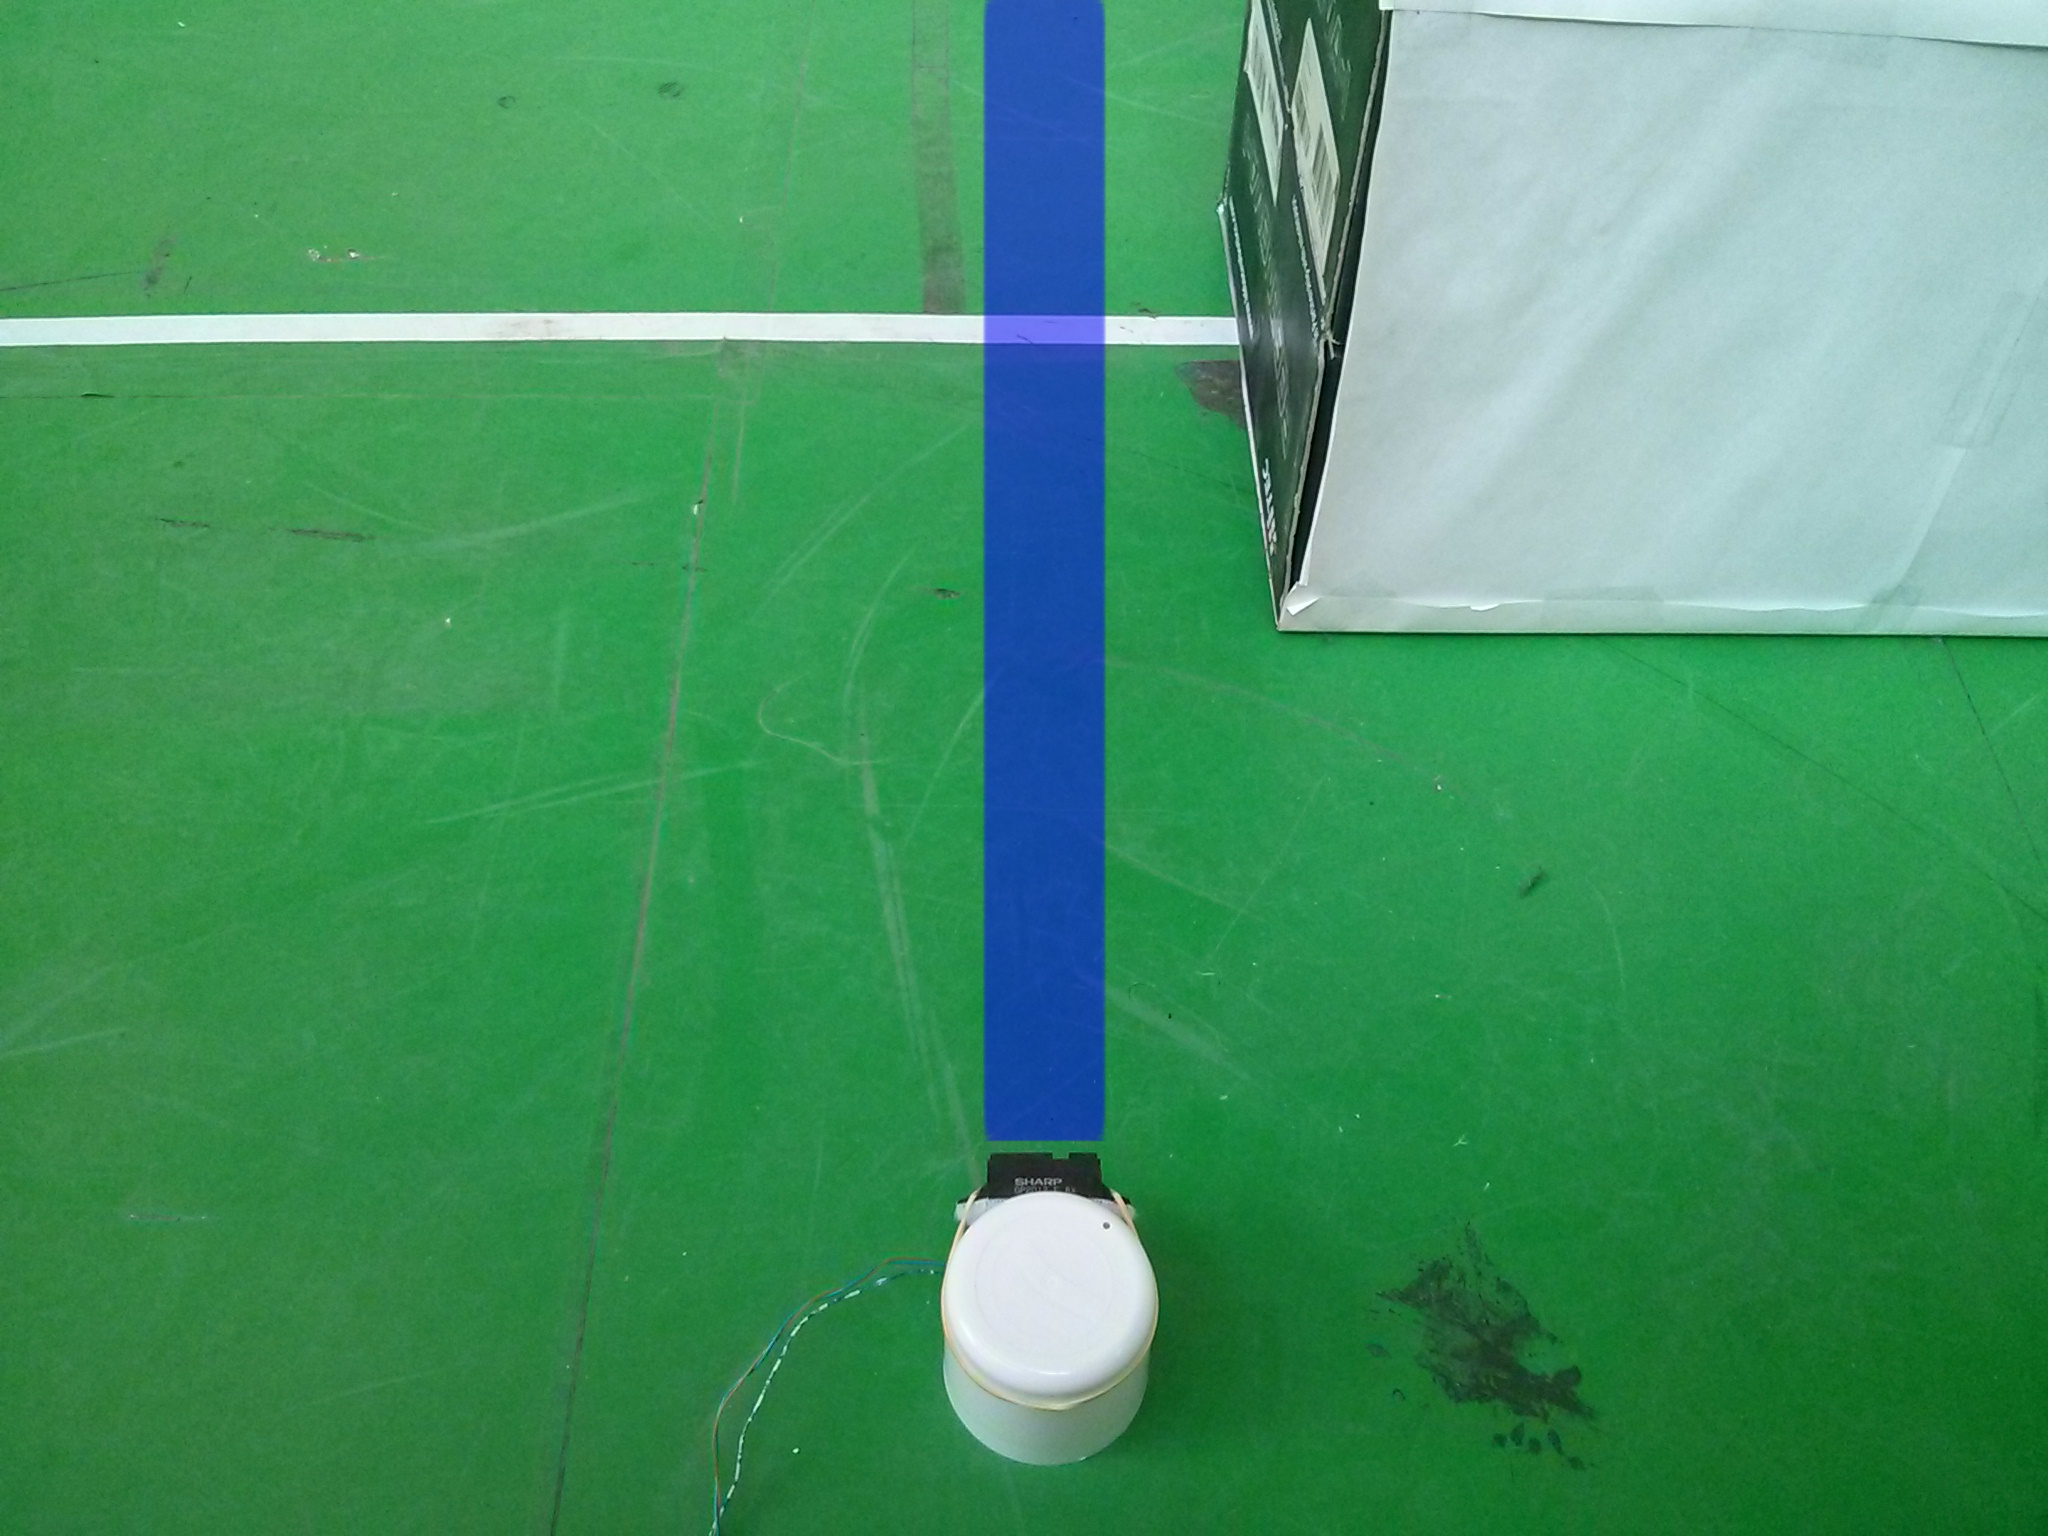
\includegraphics[width=0.5\textwidth]{figuras/expir2} & 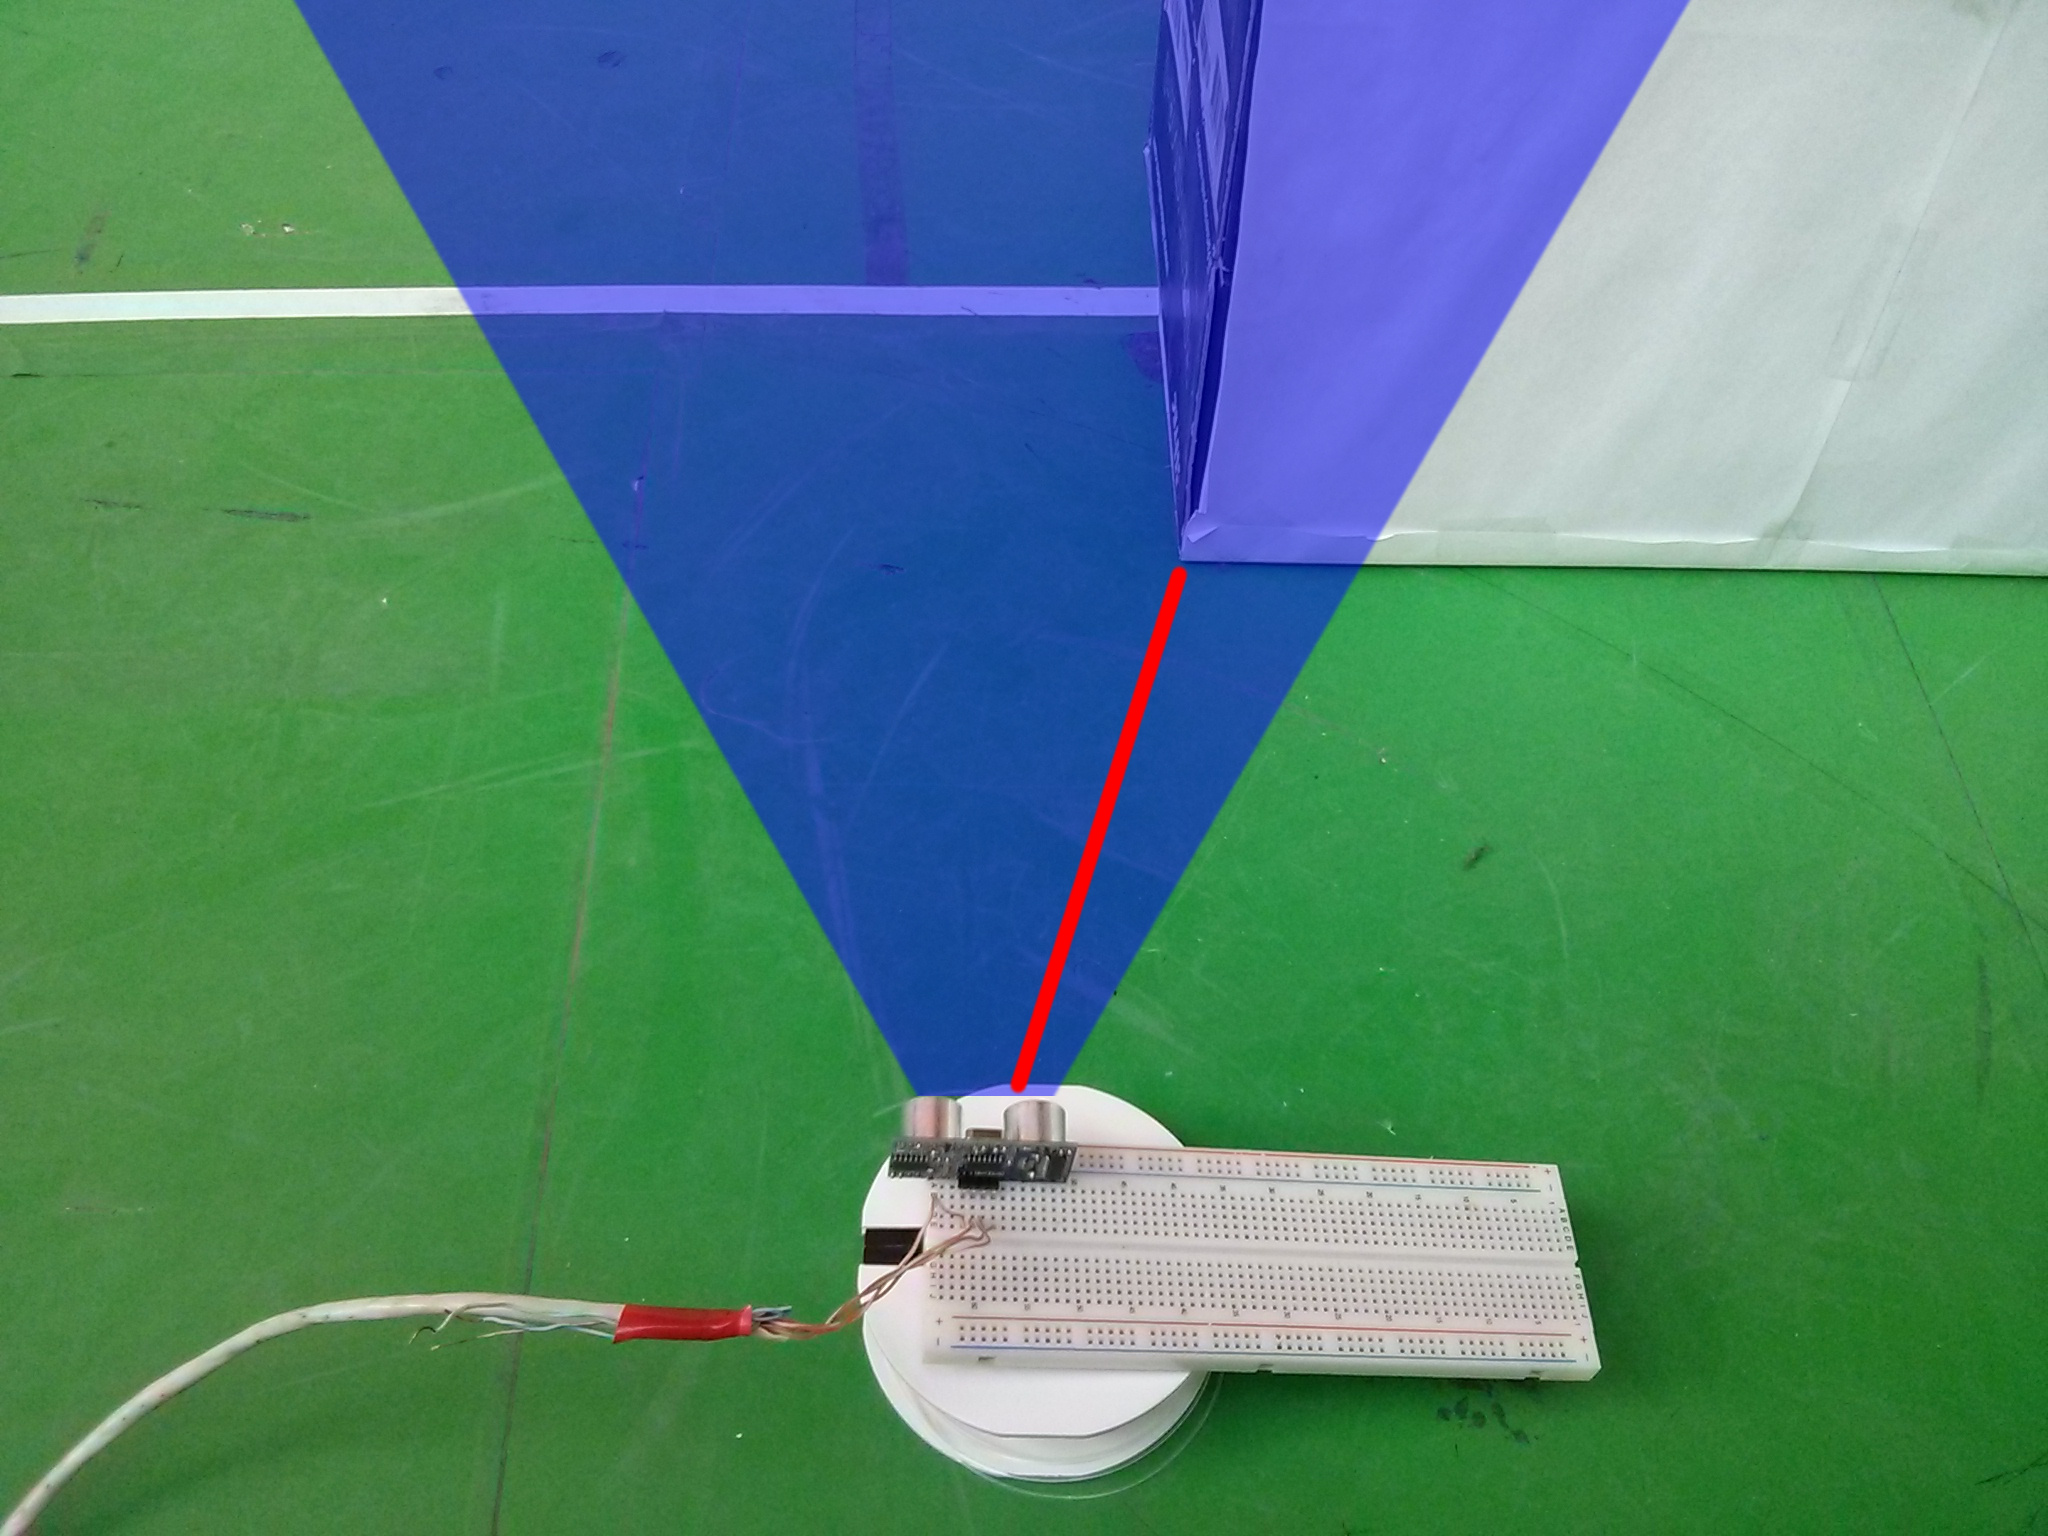
\includegraphics[width=0.5\textwidth]{figuras/expus2}  \\
\end{tabular}
\caption{Segundo experimento.}
\label{experimento2}
\end{figure} 

\begin{figure}[H]
\centering
\begin{tabular}{ >{\centering\arraybackslash}m{0.5\textwidth} >{\arraybackslash}m{0.5\textwidth}}
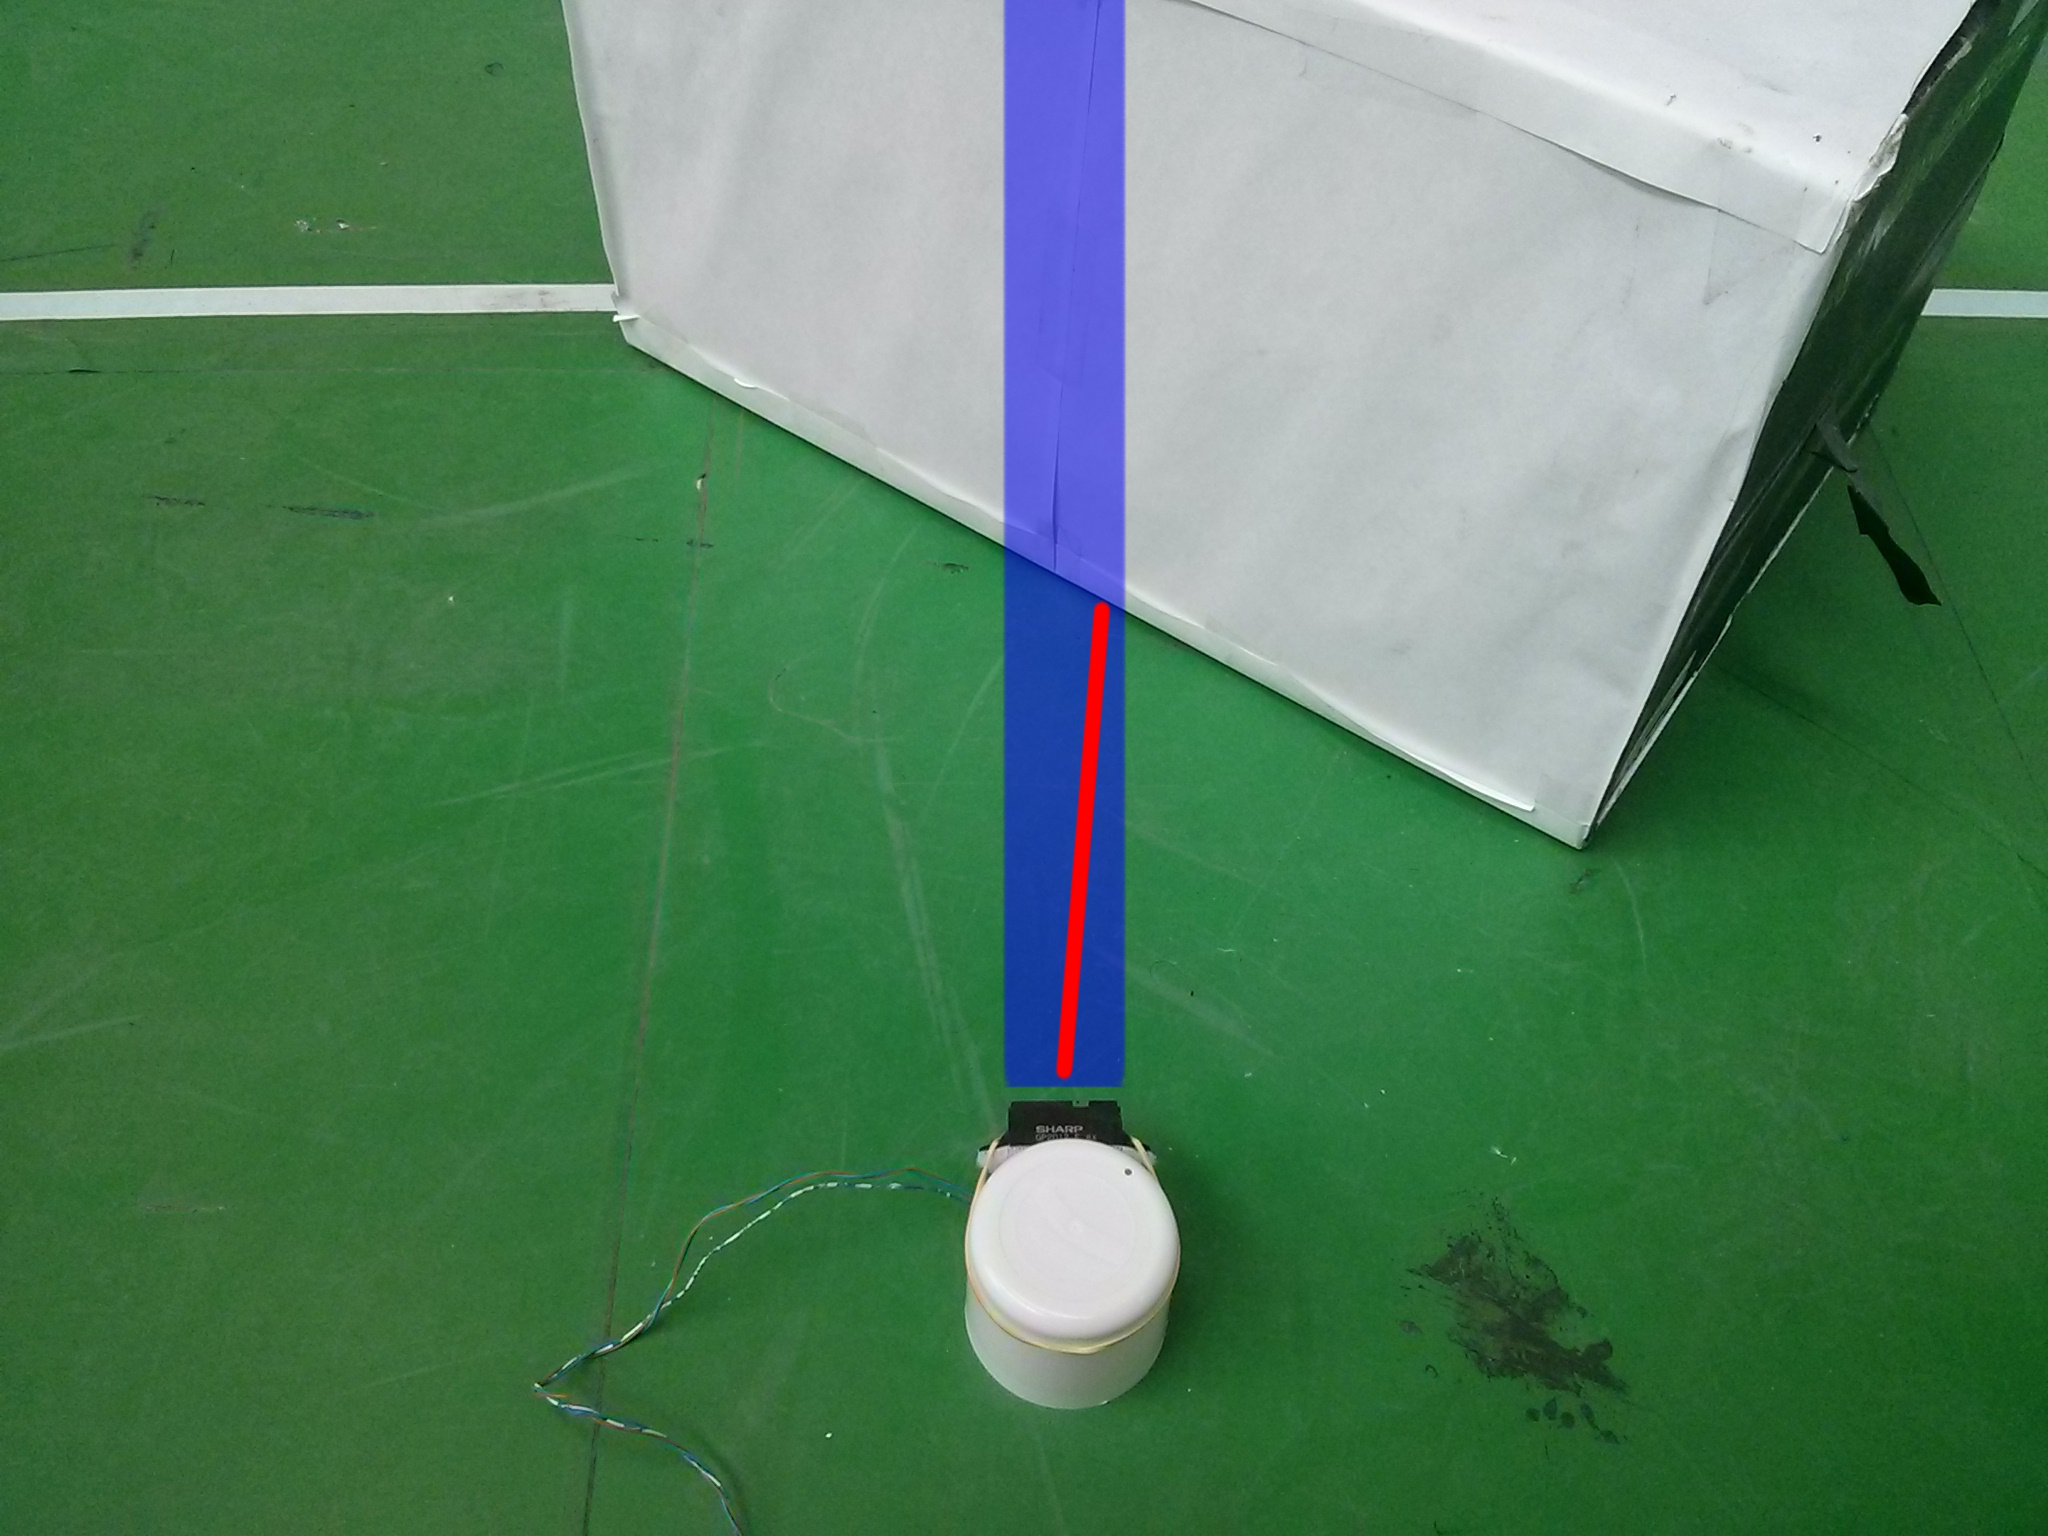
\includegraphics[width=0.5\textwidth]{figuras/expir3} & 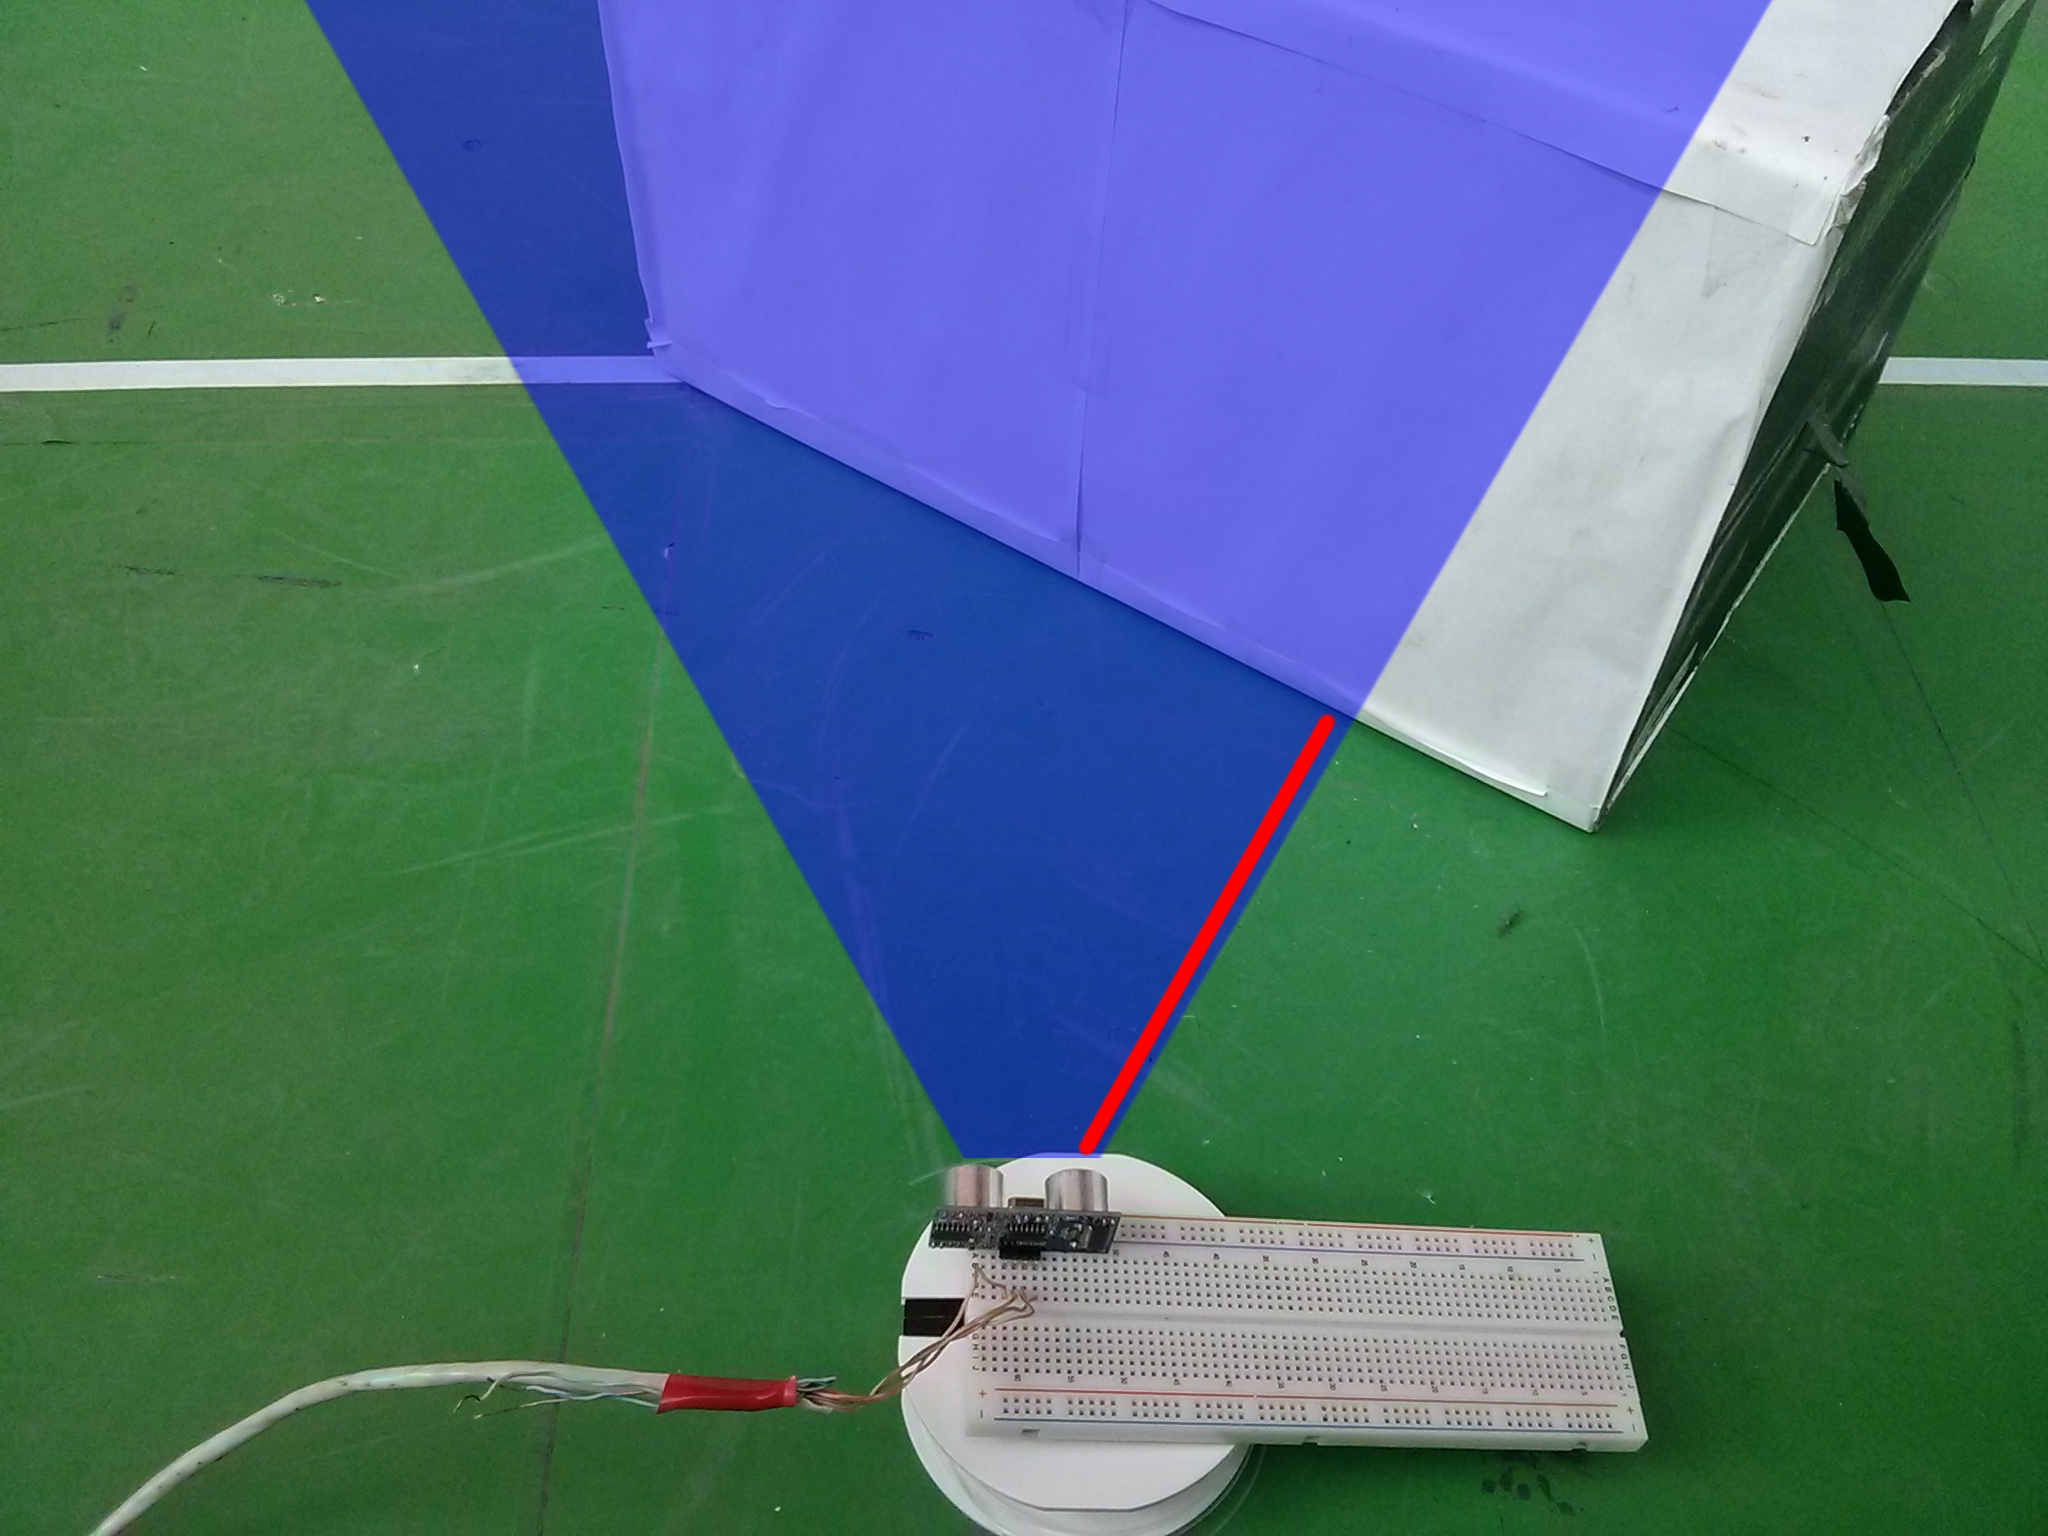
\includegraphics[width=0.5\textwidth]{figuras/expus3}  \\
\end{tabular}
\caption{Tercer experimento.}
\label{experimento3}
\end{figure} 

\subsection{Sensores inerciales TODO}

El control del equilibrio del robot es muy importante en configuraciones b�pedas, ya que estos robots son conocidos por su facilidad para tropezar y caer al suelo. Con el objetivo de analizar la posici�n del robot respecto al suelo se ha requerido la inclusi�n de diferentes sensores inerciales.

\subsubsection{Br�jula TODO}
\subsubsection{Giroscopio TODO}
\subsubsection{Aceler�metro TODO}


% TODO cambiar por foto real
\begin{figure}[H]
\centering
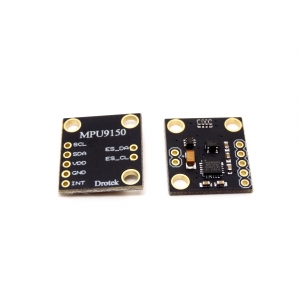
\includegraphics[width=0.8\textwidth]{figuras/imu}   
\caption{Sensor inercial MPU9150}
\label{imu}
\end{figure}

En el mercado existen varios modelos econ�micos. En este proyecto se ha utilizado un sensor MPU9150 (figura \ref{imu}), que es un sensor inercial compuesto de aceler�metro de 3 ejes, giroscopio de 3 ejes y br�jula de 3 ejes. Este sensor combina dos sensores, un MPU6050 (incluye el acelerometro y el giroscopio) y un AK8975 (incluye la br�jula).


\subsection{C�mara TODO}

La elecci�n de la c�mara ha sido condicionada principalmente por su compatibilidad con el driver de Linux v4l2. Existe una amplia variedad de c�maras v�lidas en el mercado. Dado el car�cter de este proyecto, se ha optado por utilizar una webcam, ya que son mas accesibles que las c�maras avanzadas de investigaci�n y los algoritmos de visi�n que ser�n programados no requieren im�genes de alta calidad.

\begin{figure}[H]
\centering
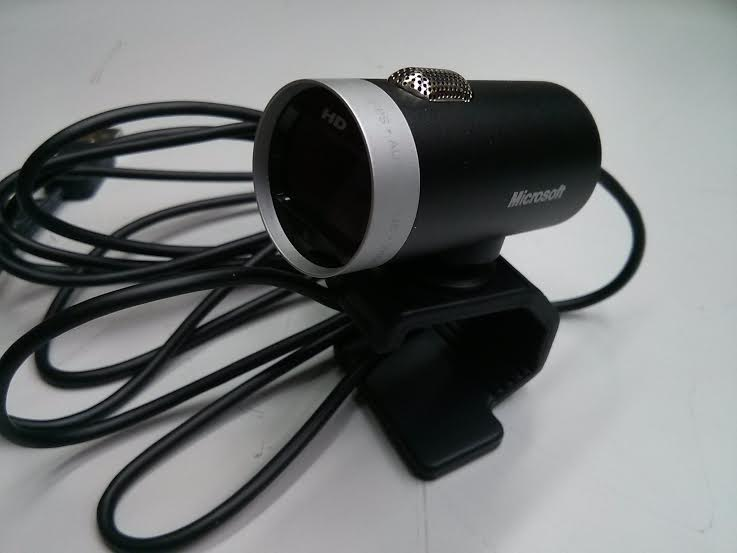
\includegraphics[width=0.8\textwidth]{figuras/camara}   
\caption{Microsoft LifeCam Cinema}
\label{camara}
\end{figure}

El modelo selecionado ha sido una Microsoft LifeCam Cinema (figura \ref{camara}). Entre sus car�cter�sticas destacan su posibilidad de grabar video en 720p HD, enfoque autom�tico y la regulaci�n de brillos en tiempo real. Adicionalmente, se trata de una c�mara de f�cil desmontaje y dimensiones contenidas, por lo que ser� sencillo integrarla en el robot.

Cabe remarcar que antes de utilizar esta c�mara se realizaron pruebas con una Hama Pocket, pero dada su baja calidad de construcci�n present� diversos problemas de fiabilidad y fue despreciada en favor de la Microsoft. 

\section{Elecci�n del controlador TODO}

Llegamos a un punto cr�tico del proyecto, y es la elecci�n de un controlador para nuestro sistema. La controlador CM-5 contenida en el kit original de Bioloid Comprehensive se encuentra muy lejos de poder soportar el conjunto de nuevos dispositivos que se usar�n en el proyecto. Necesitaremos reemplazarla por un sistema mas complejo que nos permita conectar y programar los sensores seleccionados, programar algoritmos de visi�n y comunicarse con los servos Dynamixel.

Para solucionar esto se decide colocar un SBC (Single Board Computer, ordenador de placa �nica), que dadas sus capacidades de procesamiento se utilizar� como controlador principal. As� mismo, ser� el encargado de realizar el procesamiento de im�genes. Junto al SBC, se conectar� un controlador mas sencillo basado en un microcontrolador para controlar los Dynamixel AX-12A por separado. 

De esta forma, el controlador del robot estar� formado por dos elementos, el SBC que se encargar� del procesamiento de im�genenes y sensores, y un microcontrolador se encargar� de la locomoci�n del robot.

\subsection{Controlador de locomoci�n TODO}

El controlador de locomoci�n debe encargarse de mover los 20 servos del robot y de comunicarse con el controlador de visi�n para recibir instrucciones. A continuaci�n se realiza un estudio de posibles placas que podr�an utilizarse.

\subsubsection{Arduino TODO}

Las placas Arduino se han hecho famosas por su f�cil programaci�n y puesta en marcha. Dada su popularidad, existe una gran comunidad de usuarios que generan documentaci�n de forma constante. Con una placa Arduino disponemos una amplia colecci�n de bibliotecas para interactuar con sensores y actuadores.
Sin embargo, estas placas por si solas no soportan la comunicaci�n con los servos Dynamixel. Por esta raz�n, se ha desestimado su uso en el proyecto.  

\subsubsection{Arbotix}

La placa Arbotix (figura \ref{arbotix}) est� basada, al igual que las placas Arduino, en un microcontrolador AVR. No obstante, esta placa de desarrollo est� orientada principalmente a la construcci�n de peque�os robots, por lo que posee capacidades mejores que las de las placas Arduino. Entre sus especificaciones destacan: 2 puertos serie (uno de ellos reservado para el bus Dynamixel), 32 pines de entrada/salida, 8 entradas anal�gicas, 2 drivers de 1A para motores de continua y z�calos para la conexi�n de m�dulos XBEE. 

\begin{figure}[H]
\centering
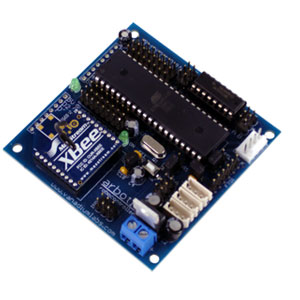
\includegraphics[width=0.6\textwidth]{figuras/arbotix}   
\caption{Placa Arbotix}
\label{arbotix}
\end{figure}

El problema de estas placas es que no existe un distribuidor que las venda en Europa. Eso no solo significa que sean dif�ciles de conseguir, sino tambien que no tienen demasiados usuarios, y por tanto la documentaci�n es escasa y heterogenea.

\subsubsection{Serie OpenCM TODO}

Recientemente la empresa Robotis ha sacado a la venta una nueva linea de placas de desarrollo, las placas OpenCM (figura \ref{cm900}). Estas placas de desarrollo est�n basadas en las placas Arduino, copiando sus funcionalidades y a�adiendo al sistema la posibilidad de comunicarse con actuadores Dynamixel. Su entorno de programaci�n est� basado en Arduino IDE y continene bibliotecas similares a las de Arduino para la comunicaci�n con sensores y actuadores. Su alta compatibilidad con Arduino proporciona al usuario una mayor facilidad a la hora de buscar documentaci�n sobre c�mo utilizar la placa.

[FOTO REAL DE CM900]

Si bien es cierto, es necesario comentar que la primera edici�n, la CM900, present� problemas en su dise�o que la conviertieron en una placa muy poco fiable y propensa a romperse prematuramente.  En este proyecto se utilizar� la OpenCM9.04, sucesora de la CM900 con similares capacidades y tama�o reducido. Entre sus especificaciones destacan: microcontrolador ARM Cortex-M3, 26 pines de entrada/salida, 10 entradas analogicas de 12 bits y 3 puertos serie (uno de ellos reservado para el bus Dynamixel).

[FOTO REAL DE OPENCM]

\subsection{Controlador de visi�n TODO}

Como controlador principal y maestro, se utilizar� un SBC. Por tama�o y capacidades existen dos alternativas directas: La Raspberry Pi B y la BeagleBone Black.

\subsubsection{Raspberry Pi TODO}

La Raspberry Pi es un ordenador completo del tama�o de una tarjeta de cr�dito, dirigida a formar parte de proyectos de electr�nica, informatica y rob�tica. Dado su bajo coste y f�cil adquisici�n, la Raspberry Pi cuenta con una comunidad de usuarios muy extensa repartida a lo largo del mundo. En internet existen colecciones de tutoriales educativos para formar al usuario y dar soporte a sus proyectos. En el cuadro \ref{raspec} se describen las especificaciones t�cnicas de la placa.

\begin{table}[H]
\centering
\begin{tabular}{ >{\arraybackslash}m{3.5cm} >{\arraybackslash}m{7.5cm}}
\hline
Especificaciones Rasp \\
\hline \hline
CPU & ARM 1176JZF\-S 700 MHz  \\ \hline
Memoria (SDRAM) & 512 MB (compartidos con la GPU)\\ \hline
Puertos USB 2.0 & 2 (v�a hub USB integrado) \\ \hline
Almacenamiento integrado & SD / MMC / ranura para SDIO \\ \hline
Perif�ricos de bajo nivel & 8 x GPIO, SPI, I2C, UART \\ \hline
Consumo energ�tico & 700 mA (3.5 W) \\ \hline
Fuente de alimentaci�n & 5 V v�a Micro USB o GPIO header  \\ \hline
Dimensiones: & 85.60mm $\times$ 53.98mm\\ \hline
Sistemas operativos soportados: &  GNU/Linux: Debian (Raspbian), Fedora (Pidora), Arch Linux (Arch Linux ARM), Slackware Linux. RISC OS2 \\ \hline
\end{tabular}
\caption{Especificaciones Raspberry Pi B}
\label{raspec}
\end{table}

En el caso que nos ocupa, ser�a una perfecta candidata a ocuparse del procesamiento de im�genes del robot, sin embargo hay algunos detalles que es importante conocer. El primer problema de la Raspberry Pi es que la l�gica de sus pines trabaja a 5V, mientras que la placa que hemos seleccionado para la parte de locomoci�n, la OpenCM, funciona a 3.3V. Esto significa que para comunicar ambas placas ser�a necesario incluir un convertidor l�gico en el sistema. Por otra parte, sus GPIOs tienen un funcionamiento puramente binario, sin entradas anal�gicas ni generaci�n de se�ales PWM. Por �ltimo, como puede observarse en la figura \ref{raspberry} aunque tiene un tama�o razonable, la placa cuenta con varios conectores de video, audio, conexion en red... etc que aunque podr�an resultar �tiles en otro tipo de proyectos, en nuestro caso estorbar�n a la hora de integrar el dispositivo en la espalda del robot.

[FOTO REAL DE UNA RASPEBRRY] TODO

\subsubsection{BeagleBone Black TODO}

La BeagleBone Black (figura \ref{beaglebone}), de Texas Instruments no es tan popular como la Raspberry Pi, sin embargo posee algunas caracter�sticas muy interesantes.

\begin{table}[H]
\centering
\begin{tabular}{ >{\arraybackslash}m{3.5cm} >{\arraybackslash}m{7.5cm}}
\hline
Especificaciones BBB \\
\hline \hline
CPU &  AM335x 1GHz ARM Cortex-A8  \\ \hline
Memoria (SDRAM) & 512 MiB \\ \hline
Puertos USB 2.0 & 1x Standard A y 1x mini B \\ \hline
Almacenamiento integrado & 4GB 8-bit eMMC / microSD \\ \hline
Perif�ricos de bajo nivel & 4xUART, 8x PWM, LCD, GPMC, MMC1, 2x SPI, 2x I2C, A/D Converter, 2x CAN bus \\ \hline
Consumo energ�tico & 1200 mA (6 W) \\ \hline
Fuente de alimentaci�n & 5 V v�a Micro USB, jack de 5.5mm a 5 V o GPIO header  \\ \hline
Dimensiones: & 86.40 mm $\times$ 53.30 mm \\ \hline
Sistemas operativos soportados: &   Fedora, Android, Ubuntu, Debian, openSUSE , �ngstr�m, FreeBSD, NetBSD, OpenBSD, QNX, MINIX 3, RISC OS, y Windows Embedded. \\ \hline
\end{tabular}
\caption{Especificaciones BeagleBone Black}
\label{blaspec}
\end{table}

Como puede observarse en el cuadro \ref{blaspec}, sus caracter�sticas son ligeramente superiores a las de la Raspberry. Principalmente, el hecho de que tenga tal variedad de pines la hace muy adecuada para usarse como controlador principal de un robot. La BeagleBone Black actualmente no cuenta con una comunidad tan extensa como la Raspberry Pi, pero cada vez se ve mas en proyectos. El problema fundamental de la BeagleBone Black es la falta de bibliotecas en C/C++ que permitan programar sus perif�ricos de bajo nivel. Esto significa que en el caso de utilizar esta placa, se deber�n programar bibliotecas propias para estos prop�sitos. 

[FIGURA DE BEAGLEBONE] TODO

Por otro lado, su l�gica funciona a 3.3V y es mas compacta que la Raspberry Pi. Por todo lo comentado, y aunque trabajar con ella pueda resultar mas tedioso que con la Raspberry Pi, se ha seleccionado la Beaglebone Black como controlador principal del robot.

\subsection{Dise�o del sistema TODO}

Una vez se ha seleccionado todos los elementos que fomar�n parte del robot, se ha dise�ado el conexionado que llevar�n. Tal y como se ha ido viendo a lo largo de este apartado, por un lado tendremos la OpenCM que se encargar� de controlar el servo PWM y los servos Dynamixel. La BeagleBone en cambio, se encargar� de recibir los datos de todos los sensores y de la c�mara. Las dos placas se conectar�n en serie. El diagrama de la figura \ref{dia1} representa las conexiones de todos los dispositivos, a excepci�n de la parte de alimentaci�n, que se ver� en la pr�xima secci�n.

\begin{figure}[H]
\centering
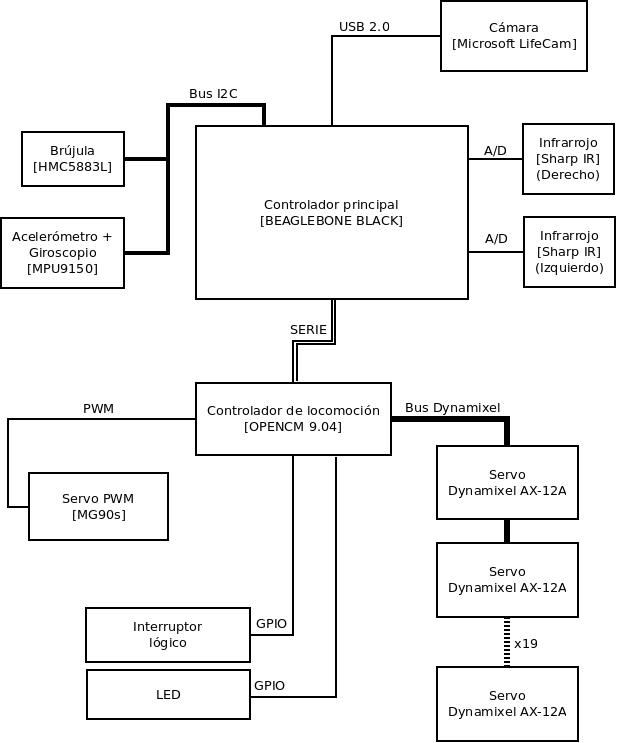
\includegraphics[width=1\textwidth]{figuras/dia1}   
\caption{Diagrama de conexiones}
\label{dia1}
\end{figure}


\section{Alimentaci�n}

La bater�a contenida en el kit es una bater�a NiMH de 8 elementos AA Sanyo Eneloop que desarrolla 9.6V y 1900mAh. Para el consumo de este robot es una opci�n aceptable que proporciona cerca de 10 minutos de autonom�a. No est� mal si se tiene en cuenta que pruebas con el CEABOT tiene una duraci�n m�xima limitada a 5 minutos. Sin embargo tiene un inconveniente, su peso y su volumen es muy alto, y al estar situado en la espalda, sube el centro de gravedad del robot de forma considerable. Esto causa inestabilidad en el robot y complica bastante la programaci�n de desplazamientos.

\subsection{Bater�a}

Por las razones descritas, se ha decidido buscar una alternativa. Los requ�sitos para seleccionar una bater�a los marcan tres factores: La tensi�n de funcionamiento de los servos, la de las placas de control y la de los sensores. Pero dado que los servos tienen una tensi�n de operaci�n en un rango de 9V a 12V, respecto al resto de elementos que ser�n alimentados a 5V o 3.3V, nos centraremos principalmente en encontrar una bater�a adecuada para los servos.

Hoy en dia, las bater�as ne NiMH est�n empezando a caer en desuso a favor de la bater�as de litio. Se barajaron dos posibilidades.

% TODO al final de la secci�n se debe calcular la autonom�a del robot

\subsubsection{Bater�as de pol�mero de litio}

Las bater�as de pol�mero de litio, mas conocidas como bater�as LiPo, destacan por desarrollar una tasa de descarga bastante alta y por tener un tama�o y peso reducido. Dado su uso en automodelismo y aeromodelismo, son unas bater�as muy comunes que en los �ltimos a�os han ido bajando su precio. Actualmente existe una gran variedad de bater�as LiPo de diversos tama�os y precio asequible. Cada c�lula LiPo ofrece 3.7V, por lo que la elecci�n correcta para este robot ser�a una bater�a de 3S, o lo que es lo mismo, 11,1V. Sin embargo, las bater�as LiPo tienen una desventaja importante, su fragilidad. El proceso de carga y descarga de una bater�a de este tipo no es un asunto trivial, una sobredescarga de la bater�a provoca un deterioro inmediato de la misma, calentando sus elementos e incluso pudiendo llegar a incendiarse. Es por ello que se necesita un cargador con capacidad para balancear las c�lulas, de forma que las tensiones de cada una de ellas se tengan bajo control durante el proceso.

\subsubsection{Bater�as de litio fosfato de hierro}  

Las bater�a de litio fosfato de hierro, es decir, LiFe, son conocidas por su gran resistencia y larga vida �til. Cada c�lula de LiFe desarrolla 3.3V y no presenta problemas por sobredescargas. De hecho, estas bater�as ni siquiera requieren de un cargador balanceador para su carga, sino que pueden cargarse sin problemas con un cargador normal. El gran problema de estas bater�as es que sus elementos son bastante voluminosos, y, al no ser tan populares como las LiPo, tampoco es demasiado f�cil encontrar modelos de tama�o y capacidad adecuados en el mercado. 

\subsubsection{Elecci�n y dise�o del sistema}  

Por su tama�o y prestaciones se ha elegido una bater�a LiPo Rhino de 3S y 1750mAh. Esta bater�a tiene unas dimensiones perfectas para montarse en la cintura del robot y su peso es 50 ( TODO pesarla, que ahora no la tengo a mano ) gramos menor al de la bater�a original (215 gramos). 

A continuaci�n se presenta una tabla (cuadro \ref{consumo}) con una estimaci�n del consumo medio de todos sus elementos.

% TODO foto de la bater�a

\begin{table}[H]
\centering
\begin{tabular}{ >{\arraybackslash}m{2cm} >{\centering\arraybackslash}m{1.3cm}  >{\arraybackslash}m{5cm}  >{\arraybackslash}m{3cm}}
\hline
Dispositivo & N�mero & Consumo unitario & Consumo total  \\
\hline \hline
Dynamixel AX-12A & x19 & $11.1V\cdot600mA=6660mW$ & $126540mW$ \\ \hline
Tower Pro MG90s & x1 & $5V\cdot120mA=600mW$ & $600mW$ \\ \hline
BeagleBone Black & x1 & $5V\cdot1200mA=6000mW$ & $6000mW$ \\ \hline
OpenCM 9.04 & x1 & $11.1V\cdot90mA\simeq1000mW$ & $1000mW$ \\ \hline
Sharp IR & x2 & $5V\cdot30mA=150mW$ & $300mW$ \\ \hline
MPU9150 & x1 & $3.3V\cdot15mA\simeq50mW$ & $50mW$ \\ \hline
HMC5883L &  x1  &  $3.3V\cdot12mA\simeq40mW$ & $40mW$ \\ \hline
Microsoft LifeCam & x1  &  $5V\cdot200mA=1000mW$ &  $1000mW$ \\ \hline \hline 
\medskip Total &  &  & \medskip $135530mW\simeq136W$  \\ \hline
\hline
\end{tabular}
\caption{Consumo medio}
\label{consumo}
\end{table}

Por tanto, la estimaci�n de autonom�a del robot en funcionamiento es la siguiente:
\[ \dfrac{11.1V\cdot1750mAh}{135530mW}\cdot\dfrac{60min}{h}\simeq8.6min\]

Entre 8 y 9 minutos de autonom�a te�ricos es un buena cifra contando con el tama�o del robot y sus prestaciones. Como conclusi�n podemos remarcar el hecho de que gracias al nuevo sistema de alimentaci�n hemos podido introducir los dispositivos necesarios para cumplir los requerimientos de este proyecto sin comprometer la autonom�a del robot.

\subsection{Regulador de tensi�n}

Hasta aqu� parece que es suficiente con la elecci�n de la nueva bater�a, sin embargo, a�n falta un detalle que deberemos resolver. La mayor parte de los dispositivos que forman el conjunto est�n alimentados a 5V. La bater�a que hemos elegido tiene una tensi�n de 11.1V, y se ha observado, que cuando est� cargada al m�ximo desarrolla hasta 12.6V. No podemos alimentar la BeagleBone Black y el resto de componentes a una tensi�n tan alta, por lo que ser� necesario colocar un regulador que nos proporcione 5V.

\subsubsection{Regulador lineal}

La primera idea fue utilizar un peque�o circuito con un regulador lineal LM7805. El LM7805 es un componente muy com�n en los circuitos electr�nicos, ya que ofrecen una salida de 5V a partir de tensiones de entrada de hasta 35V. En principio no parecer�a muy descabellado conectar los servos AX-12A  y la placa OpenCM directamente a la bater�a, y conectar en resto de componentes a trav�s del regulador.
\medskip

No obstante existen dos problemas para realizar este montaje. El primero es que la eficiencia de este componente es muy pobre, cercana al 60\% seg�n su hoja de caracter�sticas. Esto provocar�a una disminuci�n dr�stica en el tiempo de operaci�n del robot y una disipaci�n de energia tan alta que ser�a necesario incluir un disipador. Pero el segundo problema es mas importante, el componente est� dise�ado para aportar una corriente m�xima al circuito de 1 amperio. Teniendo en cuenta los datos del cuadro \ref{consumo}, solo la BeagleBone Black ya requiere una corriente de 1.2A, y junto al resto de componentes, asciende hasta 1.7A . Un consumo superior al marcado por el fabricante puede producir fallos de funcionamiento en el componente. En este caso particular, podr�a producirse un calentamiento excesivo, que a su vez puede llegar a provocar cortocircuitos internos entre la patilla de entrada y la de salida. Las consecuencias de un fallo as� ser�an nefastas, ya que deteriorar�an los dispositivos conectados a �l.

\subsubsection{Convertidor UBEC TODO }

Un UBEC (figura \ref{ubec}) es un convertidor DC-DC de tipo reductor. Los UBEC se utilizan normalmente con bater�as de litio cuando el sistema necesita una tensi�n de alimentaci�n de 5V o 6V. Es por ello que se utilizan mucho en receptores de emisoras de radiocontrol, y gracias a esto existe una amplia variedad de UBECs asequibles en el mercado. La mayor ventaja de estos circuitos convertidores es su eficiencia superior al 90\%. Gracias a esto nuestro sistema tebndr� unas perdidas menores, no se calentar� en exceso y gozar� de una autonom�a mayor. 

[FOTO DE UBEC]

\subsubsection{Elecci�n final TODO }

Tal y como se comentaba anteriormente, nuestro sistema tiene un consumo estimado de unos 1.7A en la salida de 5V, por lo que un UBEC de 3A ser�a suficiente para proporcionar al circuito la corriente necesaria para su funcionamiento. Adicionalmente se han incluido unos condensadores en la entrada y salida del circuito para ... como ser ver� en el apartado ( TODO )

\paragraph{Palabras clave:} palabraclave1, palabraclave2, palabraclave3.
 %selecci�n de componentes

%chapter introduce un nuevo cap�tulo
\chapter{Descripci�n de las herramientas a utilizar}

\section{Herramientas de dise�o y fabricaci�n de piezas}
\subsection{OpenSCAD}
\subsection{Impresi�n 3d}
\section{Herramientas de dise�o de circuitos}
\subsection{KiCad}

\section{Herramientas de programaci�n}
\subsection{Qt Creator}
\subsection{CM9 IDE}
\subsection{CMake}


CM9 IDE es un entorno de programaci�n basado en Arduino IDE, preparada para programar placas electr�nicas de la serie OpenCM.



\subsection{OpenCV}

\paragraph{Palabras clave:} palabraclave1, palabraclave2, palabraclave3.
 %Descripcion de las herramientas a utilizar
  
\chapter{Dise�o de las partes mec�nicas TODO}

La mayor parte de las piezas que monta Raider han sido redise�adas para mejorar su funci�n y/o permitir el alojamiento de nuevos dispositivos. Adem�s, al haber sido dise�adas con OpenSCAD, ha sido posible parametrizarlas para facilitar modificaciones futuras. Acciones como agregar a una pieza un soporte para un sensor determinado son ahora mucho mas r�pidas.

\section{Cabeza}

Uno de los principales objetivos del proyecto, el tomar datos del entorno con una c�mara, requiere  el dise�o y montaje se un soporte m�vil en el que poder albergar la webcam. Se ha decidido colocar la webcam en la cabeza del robot por ser la zona mas alta del robot y por tener espacio para su libre movimiento. La cabeza estar� formada por cuatro piezas: Bancada del servo, ch�sis, tapa con ranura para el cable y soporte de la c�mara. En la imagen de la figura \ref{piezascabeza} se muestran las piezas.

\begin{figure}[h]
\centering
\begin{tabular}{ >{\centering\arraybackslash}m{0.5\textwidth} >{\arraybackslash}m{0.5\textwidth}}
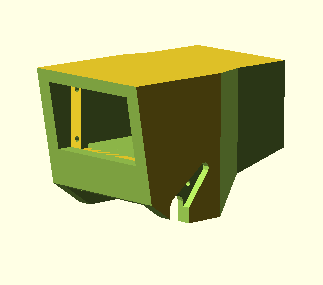
\includegraphics[width=0.4\textwidth]{figuras/cabeza} & 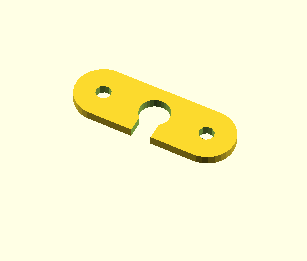
\includegraphics[width=0.4\textwidth]{figuras/tapacabeza}  \\
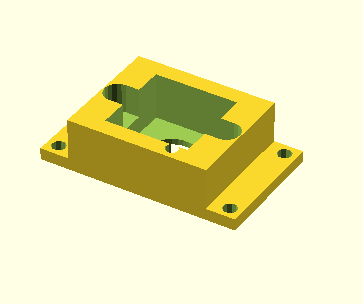
\includegraphics[width=0.4\textwidth]{figuras/chasislifecam} & 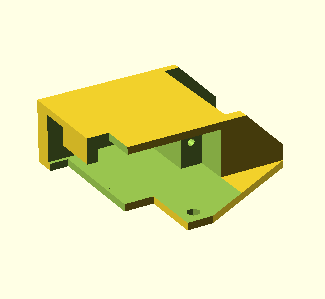
\includegraphics[width=0.4\textwidth]{figuras/cuello}  \\
\end{tabular}
\caption{Piezas necesarias para montar la cabeza}
\label{piezascabeza}
\end{figure} 
\FloatBarrier

\section{Cintura}

Como se coment� en el apartado TODO , ha sido necesario incluir un servo adicional en la cintura que permita realizar movimientos horizontales del tronco del robot respecto a la piernas. Como puede verse en la figura \ref{piezascintura}, consta de dos piezas que aprisionan el servomotor y otra mas que se utilizar� como soporte de la bater�a.

\begin{figure}[h]
\centering
\begin{tabular}{ >{\centering\arraybackslash}m{0.5\textwidth} >{\arraybackslash}m{0.5\textwidth}}
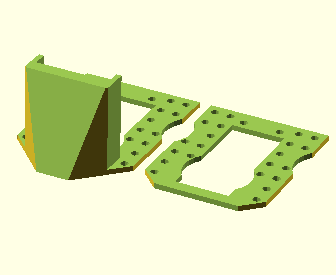
\includegraphics[width=0.4\textwidth]{figuras/cintura} & 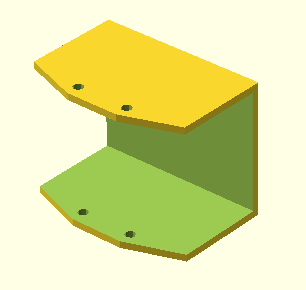
\includegraphics[width=0.4\textwidth]{figuras/soportebat}  \\
\end{tabular}
\caption{Piezas necesarias para montar la cintura}
\label{piezascintura}
\end{figure} 
\FloatBarrier 

\section{Tronco}

Para dise�ar el tronco exiten varias premisas. Necesitamos un cuerpo que permita albergar el nuevo controlador, soportar los servos de los hombros, tener una zona adecuada para montar la cabeza y una base firme que permita atornillarlo al nuevo servo de la cintura. El la imagen de la figura \ref{piezastronco} se muestran las piezas necesarias para montar el tronco: Pecho, espalda y protector.

\begin{figure}[h]
\centering
\begin{tabular}{ >{\centering\arraybackslash}m{0.5\textwidth} >{\arraybackslash}m{0.5\textwidth}}
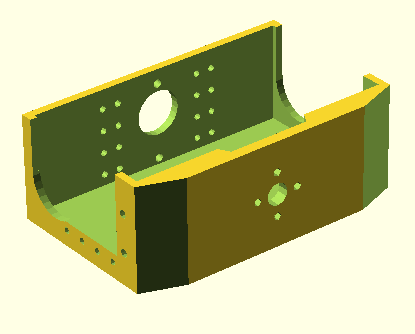
\includegraphics[width=0.4\textwidth]{figuras/pecho} & 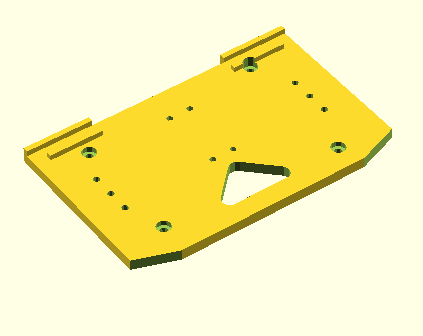
\includegraphics[width=0.4\textwidth]{figuras/espalda}  \\
\end{tabular}
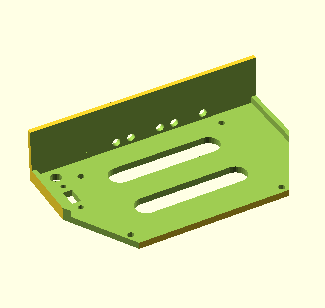
\includegraphics[width=0.4\textwidth]{figuras/protector} \\
\caption{Piezas necesarias para montar el tronco}
\label{piezastronco}
\end{figure} 
\FloatBarrier

\section{Brazos}

En este apartado se han dise�ado diferentes tramos tramos del brazo. Con ello se ha dotarle de una total modularidad, separando uniones entre servos, soportes para sensores y protectores. Gracias a esto, es muy sencillo sustituir unas piezas por otras. En este caso se han inclu�do sensores infrarrojos en los antebrazos, sin embargo, si se necesitase cambiarlos por sensores de ultrasonidos (o cualquier otro sensor) solo ser�a necesario modificar y reimprimir la bancada del sensor. En la figura \ref{piezasbrazo}

\begin{figure}[h]
\centering
\begin{tabular}{ >{\centering\arraybackslash}m{0.5\textwidth} >{\arraybackslash}m{0.5\textwidth}}
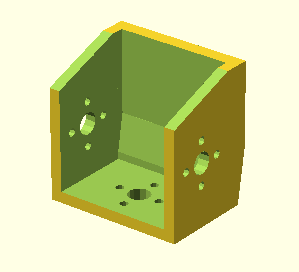
\includegraphics[width=0.4\textwidth]{figuras/hombro} & 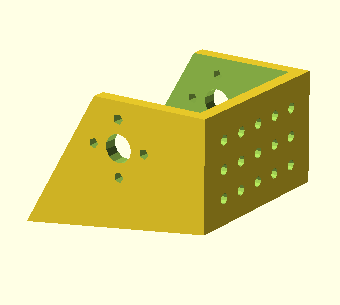
\includegraphics[width=0.4\textwidth]{figuras/codo}  \\
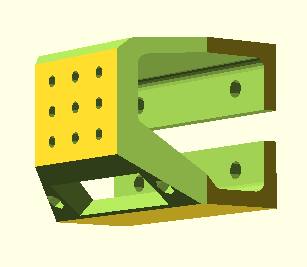
\includegraphics[width=0.4\textwidth]{figuras/antebrazo} & 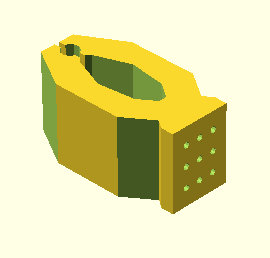
\includegraphics[width=0.4\textwidth]{figuras/gripper}  \\
\end{tabular}
\caption{Piezas necesarias para montar un brazo}
\label{piezasbrazo}
\end{figure} 
\FloatBarrier

\section{Piernas}

En cuanto a las piernas, mostradas en la figura \ref{piezaspierna}, se han modificado con dos objetivos: Rigidificar sus tramos y acortar levemente su longitud para descargar peso en las articulaciones. Al mismo tiempo, ayudar�n a bajar el centro de gravedad del robot y aumentar su estabilidad.

\begin{figure}[h]
\centering
\begin{tabular}{ >{\centering\arraybackslash}m{0.5\textwidth} >{\arraybackslash}m{0.5\textwidth}}
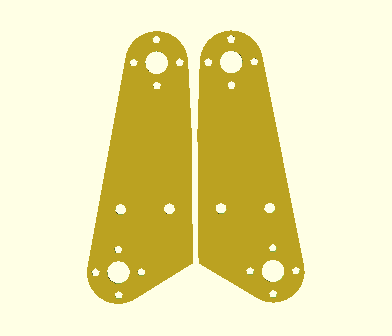
\includegraphics[width=0.4\textwidth]{figuras/pierna1} & 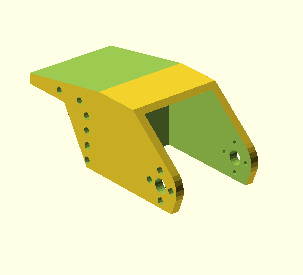
\includegraphics[width=0.4\textwidth]{figuras/pierna2}  \\
\end{tabular}
\caption{Piezas necesarias para montar una pierna}
\label{piezaspierna}
\end{figure} 
\FloatBarrier

\section{Pies y tobillos}

El dise�o de los pies se ha planteado de forma que cumpla las especificaciones del reglamento del campeonato CEABOT y al mismo tiempo tenga la mayor superficie posible. A priori, parece sencillo suponer que cuanto mayor sea la extensi�n del pie mayor ser� la estabilidad del robot, sin embargo, tambi�n es muy importante controlar como se distribuye el peso en la planta. Con el objetivo de centrar el peso en el centro del pie, se ha realizado un redise�o completo del tobillo, tal y como puede observarse en las piezas de la figura \ref{piezaspie}

\begin{figure}[h]
\centering
\begin{tabular}{ >{\centering\arraybackslash}m{0.5\textwidth} >{\arraybackslash}m{0.5\textwidth}}
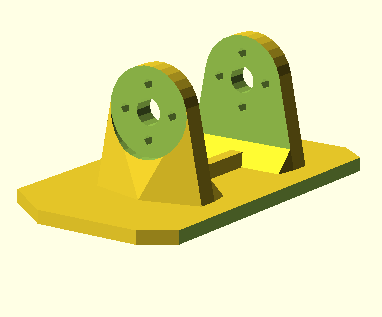
\includegraphics[width=0.4\textwidth]{figuras/pie} & 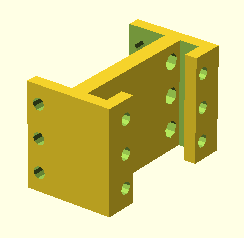
\includegraphics[width=0.4\textwidth]{figuras/tobillo}  \\
\end{tabular}
\caption{Piezas necesarias para montar un pie}
\label{piezaspie}
\end{figure}
\FloatBarrier
 %diseno mecanico

\chapter{Desarrollo y montaje}\label{chaptermontaje}

En este cap�tulo se mostrar�n los procedimientos que se han seguido para montar algunos componentes. Hasta este punto hemos definido una colecci�n de sensores, actuadores y piezas; el siguiente paso ser� integrar y conectarlos todos en el robot.

\section{Adecuaci�n de sensores}

Los sensores utilizados, tal y como se detall� en la selecci�n de componentes, ser�n: un aceler�metro y giroscopio MPU9150, una br�jula CMPS03 y dos infrarrojos Sharp. A continuaci�n se muestra c�mo han sido conectados al controlador principal, la BeagleBone Black. 

\subsection{Infrarrojos Sharp}

Los sensores infrarrojos modelo GP2Y0A21YK0F de la marca Sharp, permiten variar la tensi�n de alimentaci�n entre -0.3 y 7V, pero experimentalmente se ha observado que la mayor precisi�n se alcanza a 5V. A esta tensi�n, podemos observar en la hoja de caracter�sticas\cite{cooperationgp2y0a02yk} del sensor la gr�fica \ref{graficair}, en la que se muestra el valor de la salida del sensor respecto a la distancia medida.

\begin{figure}[H]
\centering
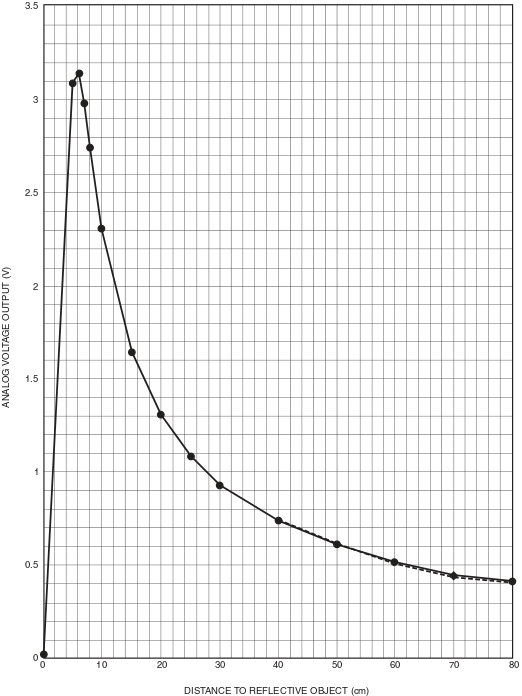
\includegraphics[width=1\textwidth]{figuras/graficair}   
\caption{Gr�fica de tensi�n entre salida para un sensor infrarrojo}
\label{graficair}
\end{figure} 

De esta gr�fica pueden sacarse dos conclusiones. La primera, ya conocida, es que la variaci�n de la salida del sensor y su medida no son proporcionales, por lo que si fuese necesaria extraer medidas en unidades reales habr�a que calcular una adecuaci�n compleja. Sin embargo, esto no ser� necesaria ya que la programaci�n del sensor se basar� en umbrales fijos que ser�n marcados de forma emp�rica. La segunda conclusi�n es que el sensor ofrecer� una tensi�n de salida m�xima de 3.3V. 

La BeagleBone Black dispone de hasta siete entradas anal�gicas como puede observarse en la figura \ref{bbbanal}. Conectaremos las salidas de los dos sensores en dos de estos pines. Sin embargo, consultando el manual de la BeagleBone Black \cite{coley2013beagleboard} observamos que cada entrada anal�gica soporta un m�ximo de 1.8V. Si alimentando el sensor a 5V lo conect�semos directamente, un pico de 3.3V podr�a deteriorar la placa. Por ello, se ha decidido aplicar una simple adecuaci�n de la salida a�adiendo un divisor resistivo. De esta forma, nos cercioraremos de que los 3.3V m�ximos que podr�an salir del sensor se conviertan en 1.8V.

\begin{figure}[H]
\centering
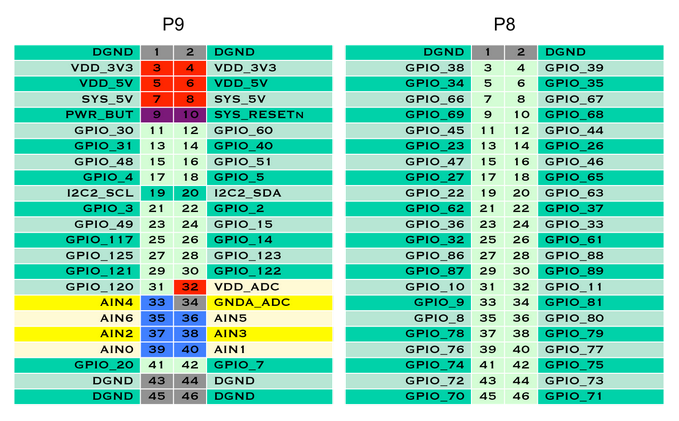
\includegraphics[width=1\textwidth]{figuras/bbbanal}   
\caption{Esquema de entradas anal�gica de una BeagleBone Black}
\label{bbbanal}
\end{figure}

En el esquema de la figura \ref{divir} podemos observar las conexiones que se han realizado entre la placa y el sensor. El sensor es alimentado a 5V a partir del convertidor DC-DC y puesto a tierra com�n con el controlador. La salida del sensor se aplicar� sobre el divisor resistivo, siendo la salida del divisor resistivo la entrada a la BeagleBone Black. Se ha colocado una resistencia de $33k\Omega$ en $Ra$ y una resistencia de $66k\Omega$ en $Rb$.

\begin{figure}[H]
\centering
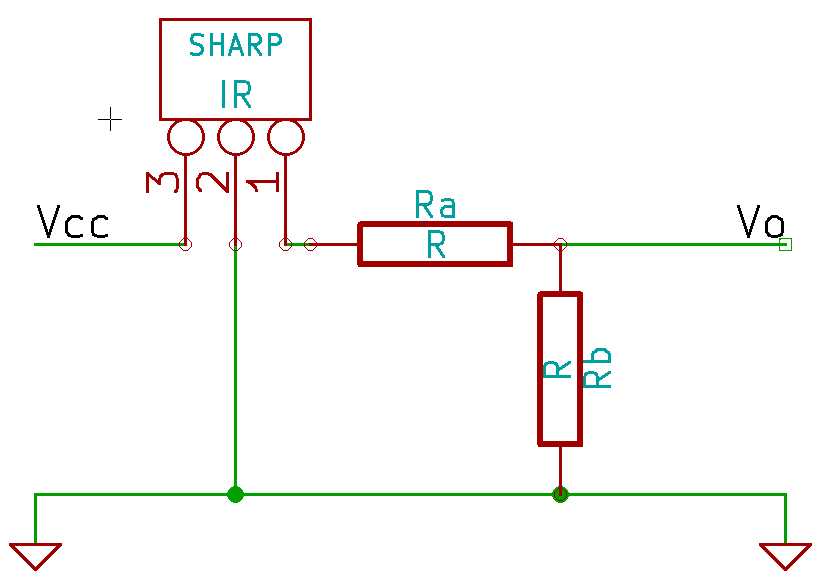
\includegraphics[width=0.65\textwidth]{figuras/divir}   
\caption{Circuito de adecuaci�n de un sensor infrarrojo}
\label{divir}
\end{figure}

\subsection{Br�jula y sensor inercial}

Tanto la br�jula CMPS03 como el sensor inercia MPU9150 han sido conectados por I2C, ambos en el mismo bus. La BeagleBone Black cuenta con dos buses I2C independientes, tal y como se observa en la figura \ref{bbbi2c}.

\begin{figure}[H]
\centering
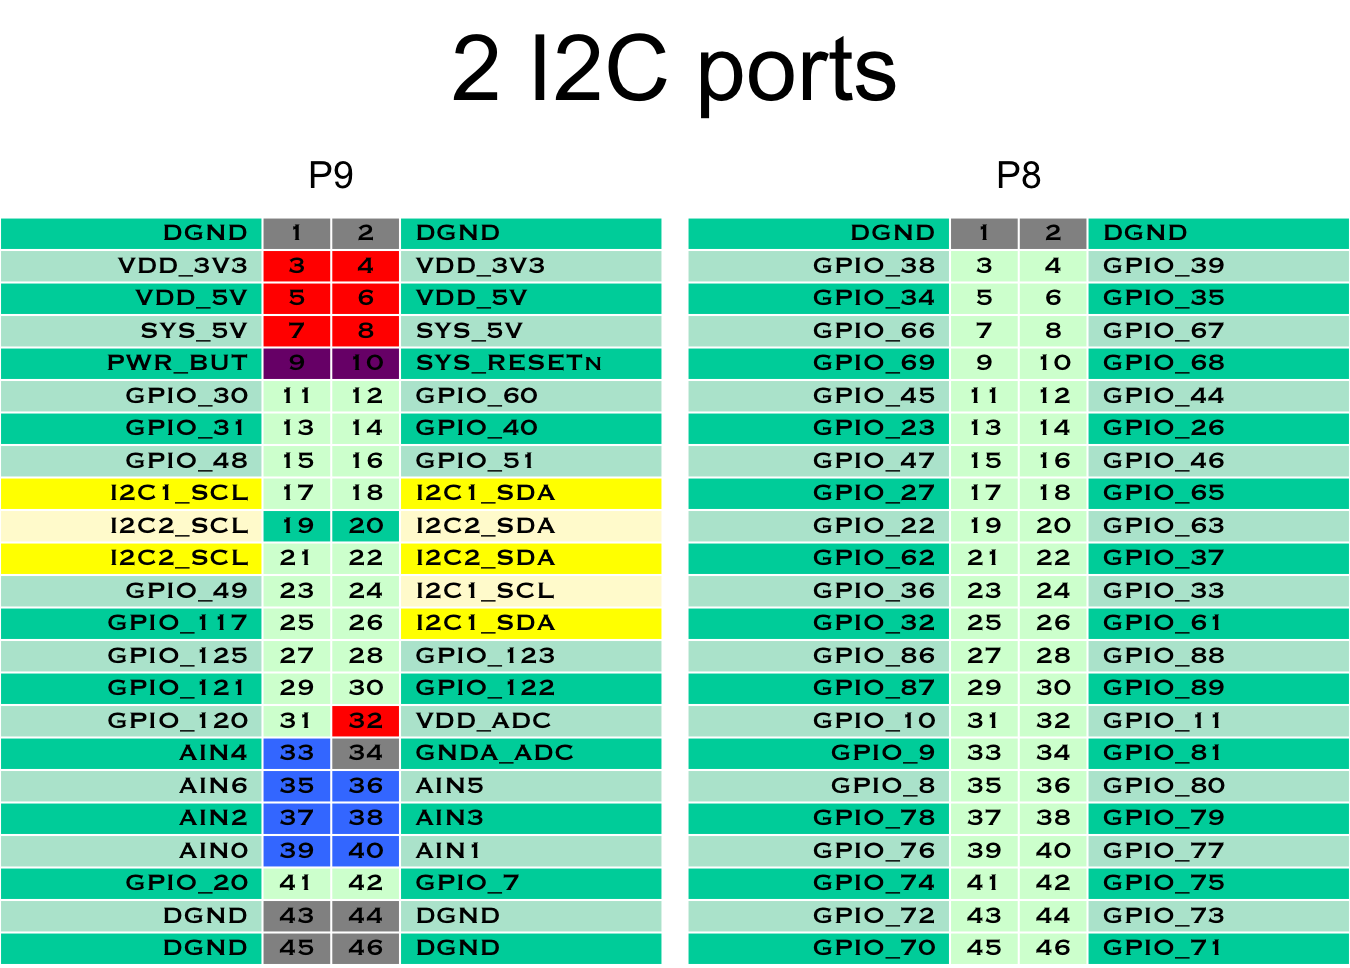
\includegraphics[width=1\textwidth]{figuras/bbbi2c}   
\caption{Esquema de puertos I2C de una BeagleBone Black}
\label{bbbi2c}
\end{figure}

De este modo el sistema ha quedado dise�ado tal y como se muestra en la figura \ref{coni2c}. Cabe destacar que los dos sensores se han alimentado a 3.3V, ya que el MPU9150 los requiere y el CMPS03, aunque se recomienda conectarlo a 5V, funciona perfectamente a 3.3V. Esta tensi�n se ha conseguido desde el pin P9-3 del controlador.

\begin{figure}[H]
\centering
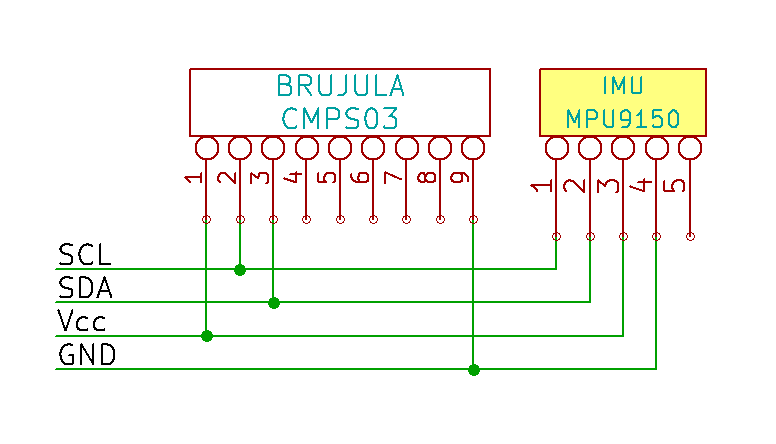
\includegraphics[width=0.85\textwidth]{figuras/esquemai2c}   
\caption{Circuito del bus I2C}
\label{coni2c}
\end{figure} 

\section{Desarrollo de una placa de expansi�n}

Para montar el esquema que se dise�� anteriormente en la figura \ref{dia1} ser� necesario cablear un gran n�mero de conexiones entre dispositivos. Para ello, se ha optado por dise�ar y fabricar una placa de expansi�n que permita conectar todos los dispositivos de una forma limpia y ordenada. Esta placa servir� para comunicar y alimentar las dos placas controladoras, sensores, actuadores y alimentaci�n de todos ellos. El esquema electr�nico puede consultarse en el anexo \ref{anexoesquematico}. A parte, el en anexo \ref{anexofotolitos} se ha inclu�do una copia de los fotolitos de la placa.


\section{Montaje}

Una vez preparados todo los componentes se ha procedido a su montaje. En los siguientes dos apartados se muestra c�mo se ha montado la placa de expasi�n y c�mo se ha integrado la webcam en la cabeza del robot.

\subsection{Montaje de la placa de expansi�n}

La placa de expansi�n ha sido fabricada mediante fresado. Tras enviar los planos a su producci�n se ha obtenido la placa que puede observarse en la figura \ref{montajeplaca1}.

\begin{figure}[h]
\centering
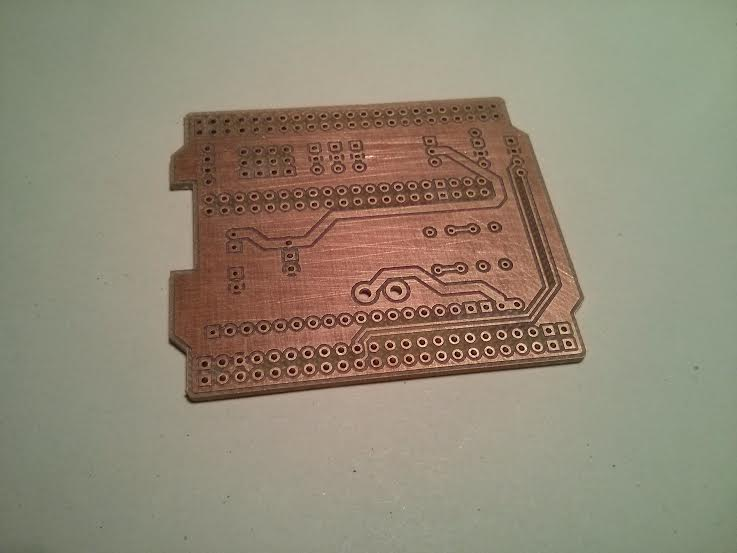
\includegraphics[width=0.5\textwidth]{figuras/montajeplaca1}   
\caption{Placa de expasi�n salida de fabricaci�n}
\label{montajeplaca1}
\end{figure}
\FloatBarrier

Tras esto se ha procedido a soldar todos los componentes que necesita. El listado de los componentes puede consultarse en el anexo TODO. En la im�gen de la figura \ref{montajeplaca2} puede observarse c�mo queda la placa una vez soldada. Adem�s, se le ha realizado un lacado de seguridad con laca aislante. Esto nos ayudar� a evitar posibles accidentes por contacto con conectores y partes met�licas del robot. Finalmente

\begin{figure}[h]
\centering
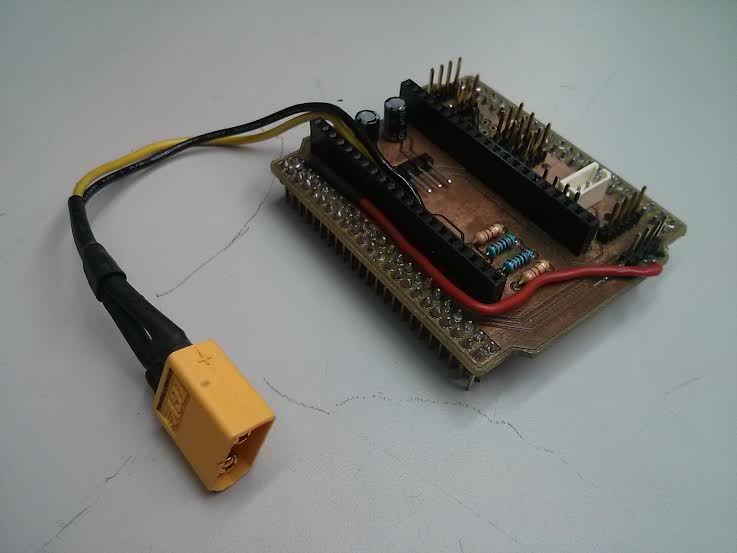
\includegraphics[width=0.5\textwidth]{figuras/montajeplaca2}   
\caption{Placa de expasi�n con componentes soldados}
\label{montajeplaca2}
\end{figure}
\FloatBarrier

\medskip En la figura \ref{montajeplaca3} puede observarse el resultado final del sistema, montado en el robot y conectado a sus componentes.

\begin{figure}[h]
\centering

\includegraphics[width=0.5\textwidth]{figuras/todo}   
\caption{Placa de expansi�n monstada en RAIDER}
\label{montajeplaca3}
\end{figure}
\FloatBarrier


\subsection{Integraci�n de la c�mara en la cabeza}

Para integrar la webcam en la cabeza de RAIDER se ha procedido a desmontar la c�mara Microsoft LifeCam con el objetivo de eliminar su carcasa. El resultado de extraer la c�mara puede observarse en la figura \ref{montajecam1}.

\begin{figure}[h]
\centering
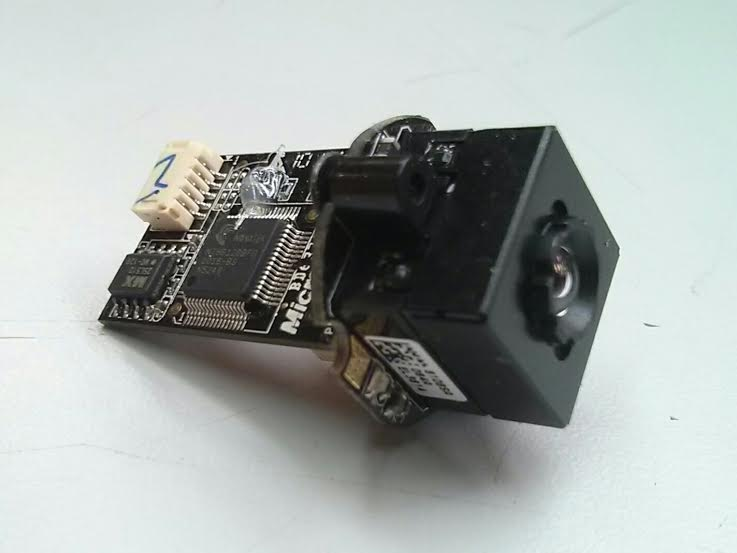
\includegraphics[width=0.5\textwidth]{figuras/montajecam1}   
\caption{C�mara Microsoft LifeCam desmontada}
\label{montajecam1}
\end{figure}
\FloatBarrier

\medskip Ahora, se pasar� a montarla en las piezas imprimibles que se dise�aron para tal efecto. Las piezas aparecen en la figura \ref{montajecam2} junto a la c�mara.

\begin{figure}[h]
\centering
\begin{tabular}{ >{\centering\arraybackslash}m{0.33\textwidth}
>{\centering\arraybackslash}m{0.33\textwidth}
>{\centering\arraybackslash}m{0.33\textwidth}}
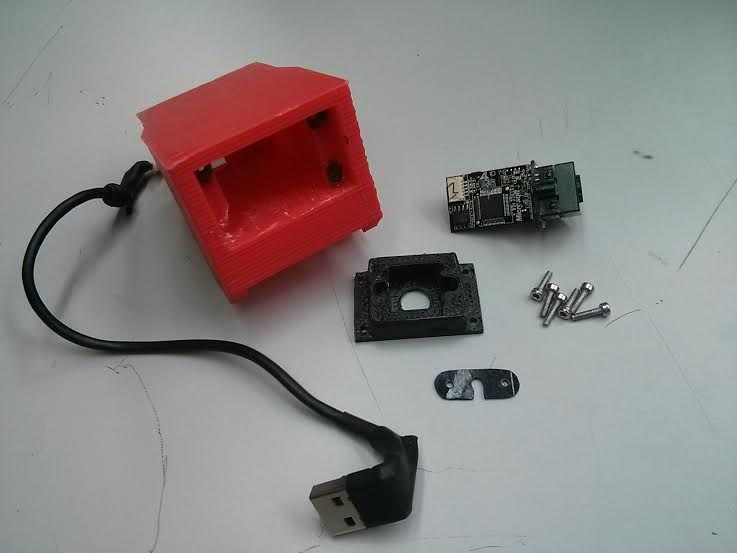
\includegraphics[width=0.33\textwidth]{figuras/montajecam2} &
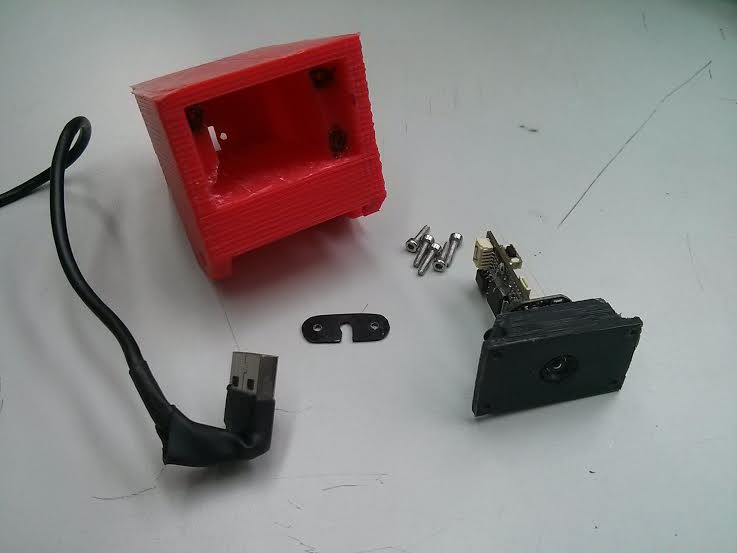
\includegraphics[width=0.33\textwidth]{figuras/montajecam3} &
\includegraphics[width=0.33\textwidth]{figuras/montajecam4} \\
\end{tabular}
\caption{Integraci�n de la c�mara en la cabeza}
\label{montajecam2}
\end{figure}
\FloatBarrier

Una vez montado y acortado el cable, procedemos a montar el servo que mover� la cabeza. Como se muestra en la figura \ref{montajecam5}, este se aloja en el cuello.

\begin{figure}[h]
\centering
\includegraphics[width=0.47\textwidth]{figuras/montajecam5}   
\caption{Cuello y soporte para la cabeza}
\label{montajecam5}
\end{figure}
\FloatBarrier

Finalmente, en la figura \ref{montajecam6} se muestra el resultado del montaje completo

\begin{figure}[h]
\centering
\begin{tabular}{ >{\centering\arraybackslash}m{0.5\textwidth}
>{\centering\arraybackslash}m{0.5\textwidth}}
\includegraphics[width=0.40\textwidth]{figuras/todo} &
\includegraphics[width=0.40\textwidth]{figuras/todo} \\
\end{tabular}
\caption{Resultado tras la integraci�n de la cabeza en el robot}
\label{montajecam6}
\end{figure}
\FloatBarrier

\subsection{Integraci�n de los sensores infrarrojos en los brazos}

Tal y como se coment� en el apartado TODO, se han integrado dos sensores en los brazos de RAIDER. El motivo de montarlos en los brazos es que se esta manera gozar�n de mayor libertad a la hora de apuntara obst�culos. As� mismo, se ha buscado que el sensor estuviese en una posici�n segura, protegido ante ca�das. En la figura \ref{montajeir1} se pueden observar los dos sensores infrarrojos junto a las piezas que se han dise�ado para alojarlos.

[FOTO de sharps y piezas]
\begin{figure}[h]
\centering
\includegraphics[width=0.5\textwidth]{figuras/montajeir1}   
\caption{Sensores infrarrojos y soportes}
\label{montajeir1}
\end{figure}
\FloatBarrier

Tras montar las piezas, se ha obtenido el resultado mostrado en la figura \ref{montajeir2}

[FOTO del conjunto]
\begin{figure}[H]
\centering
\includegraphics[width=0.5\textwidth]{figuras/todo}   
\caption{Brazos con sensores montados}
\label{montajeir2}
\end{figure}
\FloatBarrier



%chapter introduce un nuevo cap�tulo
\chapter{Programaci�n TODO}

En este cap�tulo se presenta el desarrollo de todo el software que ha sido requerido preparar para la puesta en marcha del robot.

\section{Configuraci�n de la BeagleBone Black TODO}

De fabrica... TODO

\subsection{Sistema operativo}

El controlador principal, la BeagleBone Black, trae de f�brica una instalaci�n de una distribuci�n �ngstr�m basada en Linux. El sistema operativo incluye: entorno gr�fico, escritorio, OpenCV 2.2 y otros programas como navegadores o reproductores de archivos multimedia. Esto se debe a que la BeagleBone Black no es una placa que de f�brica est� pensada para su uso en robots, sino que constituye un ordenador completo que puede adquirir la funci�n de centro multimedia, equipo de ofim�tica o incluso servidor de una red.

\medskip La distribuci�n �ngstr�m no es una de las m�s populares entre los sistemas operativos basados en Linux, no cuenta con una comunidad de usuarios tan amplia como Debian o Fedora. Por ello, las actualizaciones no suelen ser muy frecuentes y, en muchos casos, el sistema presenta errores de funcionamiento a la hora de realizar tareas b�sicas, como la instalaci�n de nuevo software.

\medskip Por esta razones se ha decidido instalar un nuevo sistema operativo. Se pretende conseguir una distribuci�n de Linux que solo tenga lo m�nimo necesario que requiere el robot para su funcionamiento. Con este objetivo, se instala en la BeagleBone Black una distribuci�n Debian.

\subsection{Instalaci�n de librer�as TODO}

Para la realizaci�n del proyecto, se ha requerido instalar Git, CMake, Video4Linux2 y las librer�as de OpenCV 2.4.8 y ZBar 0.1.

\medskip Antes de comenzar con la instalaci�n de software, es recomendable realizar una actualizaci�n del sistema ejecutando los siguientes comandos:

\begin{verbatim}
sudo apt-get update
sudo apt-get upgrade
\end{verbatim}

\bigskip  Lo primero que instalaremos ser� Git, ya que lo necesitaremos para instalar algunas librar�as posteriormente. Git se instala ejecutando el siguiente comando: 
\begin{verbatim}
sudo apt-get install git-core
\end{verbatim}

\bigskip Para instalar CMake lo haremos de la siguiente forma:

\begin{verbatim}
sudo apt-get install cmake
sudo apt-get install cmake-curses-gui
\end{verbatim}

\bigskip Para el control y configuraci�n de la webcam se necesitar� el driver Video4Linux. Se instalar� como se muestra a continuaci�n:

\begin{verbatim}
sudo apt-get install v4l-utils
\end{verbatim}


\bigskip  Una vez hecho esto, se pasar� a instalar las librer�as que se utilizar�n en el c�digo del robot. La forma mas sencilla de instalar Zbar ser� hacerlo desde los repositorios de Debian. De este modo, ejecutaremos los siguientes comandos:
\begin{verbatim}
sudo apt-get install libzbar0
sudo apt-get install libzbar-dev
\end{verbatim}

\bigskip  Por �ltimo, instalaremos OpenCV. Se comenzar� por descargar todas las librar�as que requiere OpenCV. Se instalar�n una a una de la siguiente forma:
\begin{verbatim}
sudo apt-get install build-essential 
sudo apt-get install libgtk2.0-dev 
sudo apt-get install pkg-config 
sudo apt-get install python-dev 
sudo apt-get install python-numpy 
sudo apt-get install libavcodec-dev 
sudo apt-get install libavformat-dev 
sudo apt-get install libswscale-dev
\end{verbatim}

Hecho esto, se proceder� a descargar la �ltima versi�n estable del c�digo, que en este momento es la 2.4.9.

\begin{verbatim}
wget http://downloads.sourceforge.net/project/opencvlibrary/opencv-unix/2.4.9/opencv-2.4.9.zip
\end{verbatim}

\bigskip Y posteriormente se instalar� de este modo:

\begin{verbatim}
unzip opencv-2.4.9.zip
cd opencv-2.4.9
mkdir build
cd build
cmake -D CMAKE_BUILD_TYPE=RELEASE -D CMAKE_INSTALL_PREFIX=/usr/local ..
make
sudo make install
\end{verbatim}

\subsection{Configuraci�n de la c�mara}

A continuaci�n se configurar� la webcam en la beaglebone. Para esto se conectar� por USB la Microsoft Lifecam a la BeagleBone Black tal y como puede observarse en la figura \ref{robotbbbcam}. A partir de aqu�, se iniciar� sesi�n en la BeagleBone Black y se proceder� a configurar la c�mara.

\medskip Lo primero que se har� ser� comprobar que la c�mara se ha reconocido correctamente. Para ello ejecutaremos el comando:

\begin{verbatim}
lsusb
\end{verbatim}

\bigskip Y deber� proporcionarnos una salida parecida a la que puede observarse en la figura \ref{lsusbbbb}. La salida indica que la webcam est� conectada en el bus 001

\begin{figure}[h]
\centering
\includegraphics[width=1\textwidth]{figuras/lsusbbbb}   
\caption{Salida del comando lsusb}
\label{lsusbbbb}
\end{figure}

\medskip Para cerciorarno de que la c�mara se ha reconocido correctamente podemos buscarla en el directorio /dev. En la siguiente imagen (figura \ref{lsdev}) se observa el archivo /dev/video0, que est� vinculado a la webcam.

\begin{figure}[h]
\centering
\includegraphics[width=1\textwidth]{figuras/lsdev}   
\caption{Comprobaci�n de conexi�n para la webcam}
\label{lsdev}
\end{figure}

A continuaci�n nos ayudaremos de las utilidades de Video4Linux (una interfaz para la programaci�n de aplicaciones con captura de im�genes para Linux) para la webcam. OpenCV se apoya en Video4Linux, por tanto, lo primero que se har� ser� comprobar que la c�mara es compatible con Video4Linux. Para ello, se ejecutar� el siguiente comando:

\begin{verbatim}
v4l2-ctl --list-devices
\end{verbatim}

\bigskip Tras ejecutarlo se deber� observar una salida similar a la de la figura \ref{v4llist}

\begin{figure}[h]
\centering
\includegraphics[width=1\textwidth]{figuras/v4llist}   
\caption{Comprobaci�n de compatibilidad para la webcam}
\label{v4llist}
\end{figure}

�sto nos confirma que la c�mara funciona correctamente. Para proseguir con la configuraci�n vamos a ejecutar el comando siguiente:

\begin{verbatim}
v4l2-ctl --all
\end{verbatim}

\bigskip  En la figura \ref{v4lall} podemos observar la salida del comando. En ella se pueden observar diferentes par�metros como el formato de video, la resoluci�n o los fotogramas por segundo.

\begin{figure}[h]
\centering
\includegraphics[width=1\textwidth]{figuras/v4lall}   
\caption{Par�metros le�dos de la c�mara}
\label{v4lall}
\end{figure}

\medskip Por �ltimo, se bajar� la resoluci�n de la c�mara a un valor que nos permita tratar las im�genes con mayor rapidez cuando se programen algoritmos de visi�n con OpenCV desde la BeagleBone Black. Se ha elegido una resoluci�n de 320x240, mas adelante se ajustar� este valor emp�ricamente en funci�n del rendimiento del robot. Para ello ejecutamos este comando de configuraci�n:

\begin{verbatim}
v4l2-ctl --set-fmt-video=width=320,heigth=240
\end{verbatim}

\bigskip  Tras estos pasos la c�mara ya est� preparada y lista para usarse.

%vdeo capture aplication progamin interface for linux

\subsection{Programaci�n de scripts de configuraci�n TODO}



\section{Sistema de locomoci�n TODO}

Antes de comenzar con esta secci�n, es importante se�alar algunos detalles importantes. Si bien es cierto, el control del robot girar� en torno a un algoritmo de visi�n, su funcionamiento de apoyar� en un control de locomoci�n robusto que permita al robot realizar desplazamientos seguros sobre el terreno. Por tanto, dado que se trata de un robot b�pedo, la programaci�n de movimientos no es un tema trivial como lo podr�a ser en un robot con ruedas.

Para conseguir que Raider pueda moverse con soltura se han seguido varios pasos, cada cual de un nivel superior al anterior.

\subsection{Movimiento del servo PWM}
% aqui no explicar el principio de funcionamiento, solo la parte de programacion
% o sea, de Servo.write para arriba

El control del servo PWM de Raider, situado en su cabeza, se realiza con la biblioteca Servo.h orginalmente desarrolladas para Arduino y que posteriormente ha sido portada para su utilizaci�n en OpenCM. Dado el cometido de este servo, no ser� necesario realizar un control de su velocidad, por lo que un simple control de su posici�n ser� suficiente.

La biblioteca Servo.h nos permite controlar el movimiento de un servo a partir de un valor de posici�n, y se encarga de producir la se�al PWM correspondiente. Aunque los m�todos utilizados pueden encontrarse en la documentaci�n de Arduino ( TODO ), a continuaci�n introduzco una breve explicaci�n de los que han sido utilizados en este proyecto:

\subsubsection{Servo::attach(uint8 pin)}

Con esta funci�n configuramos un pin de la OpenCM para que act�e como emisora de se�ales PWM. A partir de esta inicializaci�n ya puede moverse el servo.

\subsubsection{Servo::writeMicroseconds(uint16 pulseWidth)}

Para mover el servo se utiliza la funci�n writeMicroseconds, cuyo par�metro define la amplitud  del pulso de la onda PWM. Si bien es cierto, existe otra funci�n paralela llamada write(int angle) que directamente utiliza como par�metro la posici�n en grados, se ha utilizado writeMicroseconds por su mayor precisi�n. Acepta valores de entre 1000 y 2000 microsegundos, pero para mantener un formato constante con el resto de articulaciones, se ha realizado una conversi�n matem�tica a un rango de 0 a 1023.

\subsection{Movimiento de los actuadores Dynamixel}

Para comunicarse con los actuadores Dynamixel (de los que hablamos en TODO ) debemos utilizar su protocolo particular. Los servos son controlados mediante el envio de paquetes de datos binarios. Existen dos tipos de paquetes en el protocolo: Los paquetes de instrucciones, que son los que envia el controlador a los servos; y los paquetes de estado, que son los los servos env�an al controlador.

\medskip 
Cada servo tiene una ID, o dicho de otra forma, un n�mero de identidad propio e irrepetible que identifica a un servo particular dentro del bus. La comunicaci�n en el bus se realiza mediante el intercambio de paquetes de instrucciones y estados con una ID concreta.
Por esta raz�n, en un mismo bus no deben existir servos con la misma ID, ya que provocar�n colisiones entre los paquetes e impedir�n el correcto funcionamiento del sistema. Sin embargo, estas ID son f�cilmente reprogramables y pueden modificarse realizando una escritura sobre el registro 3 (0X03).

\medskip 
El protocolo de comunicaci�n utilizado es una comunicaci�n serie as�ncrona de 8 bits, con 1 bit de Stop y sin paridad. La conexi�n, de tipo Half Duplex, no permite la transmision y recepci�n de paquetes de forma simultanea. Esto la convierte en una conexi�n bastante t�pica en los sistema que utilizan un solo bus de comunicaci�n. Como en el mismo bus existe mas de un dispositivo, todos deben permanecer en modo de escucha salvo el que est� transmitiendo en ese instante. El controlador principal, la placa OpenCM 9.04, asigna la direcci�n del bus en modo escucha, y solo cambia la direcci�n del bus a modo de envio mientras manda un paquete. (TODO revisar) Los Dynamixel AX-12A poseen una tabla de registros (tabla TODO ) sobre la cual podemos modificar varios par�metros referente a su estado y su funcionamiento. La tabla de registros puede consultarse en TODO .

\medskip 
Para realizar una rotaci�n simple en un servomotor, ser�a suficiente con escribir en el registro 32 (Goal Position) un valor comprendido entre 0 y 1023, y el servo se situar� inmediatamente en esa posici�n. Sin embargo, existen otros par�metros interesantes en el mapa de registros que conviene controlar, como la posici�n instantanea, la velocidad de giro, el consumo el�ctrico o incluso la temperatura del dispositivo.

\medskip 
Para mover los 19 AX-12A de Raider se utilizan los par�metros de posici�n objetivo (Goal Position) y velocidad de giro (Moving Speed) de forma combinada. Dado que est� programaci�n se ha realizado desde la OpenCM 9.04 se ha utilizado la biblioteca Dynamixel.h, que funciona como una macro para leer y escribir en los registros de forma sencilla y eficiente. Dentro de la biblioteca utilizaremos la funci�n writeWord con la siguiente sintaxis:

% TODO arreglar codigos

\begin{verbatim}
Dxl.writeWord(
	Dynamixel_Motor_Number,	
	Address_Number,
	Address_Data
);
\end{verbatim}

A modo de ejemplo, para asignar una velocidad de $3.5rad/s$ al servo con la ID 5, primero calcular�amos el valor correspondiente para una resoluci�n de 10 bits. Seg�n el manual de los servos Dynamixel ( TODO citar) AX-12A, la velocidad m�xima de estos servomotores es de $114rpm$. Por tanto, se realizar�a la siguiente conversi�n:

\[ 3.5 \cdot \frac{rad}{s} \cdot \frac{60 s}{2 \pi rad} \cdot rpm \cdot \frac{1024}{114 rpm}= 300.216 \simeq 300 \]

\medskip
Dentro del c�digo, utilizaremos la funci�n writeWord para asignar este valor en el registro 32 (Moving Speed):

% TODO arreglar codigos
\begin{verbatim}
Dxl.writeWord(5,32,300);
\end{verbatim} 

Seguidamente, asignar�amos al servo una posici�n final siguiendo el criterio de la figura \ref{goalposition}

\begin{figure}[h]
\centering
\includegraphics[width=0.55\textwidth]{figuras/goalposition}   
\caption{Amplitud de giro de un AX-12A}
\label{goalposition}
\end{figure}

Continuando con el ejemplo, calcularemos el valor que debemos darle al registro para mover el servo a una posici�n de $120�$, teniendo en cuenta que las especificaciones nos indican una amplitud de giro total de 300� reales con una resoluci�n de 10 bits. De esta forma, har�amos la siguiente conversi�n:

\[ 120� \cdot \frac{1024}{300�}= 409.6 \simeq 410 \]

\medskip
En nuestro programa escribir�amos en el registro 30 (Goal Position) de la siguiente forma:

% TODO arreglar codigos
\begin{verbatim}
Dxl.writeWord(5,30,410);
\end{verbatim} 

Como resumen, con estos pasos hemos conseguido mover el servo con la ID 5 (Que corresponde al codo del brazo izquierdo de Raider), a una posici�n de $120�$ con una velocidad de $3.5 rad/s$

\subsection{Movimiento sincronizado de las articulaciones}

En el apartado anterior se ha mostrado c�mo se realiza el movimiento de un servo, sin embargo, para mover el cuerpo del robot necesitaremos mover todos al mismo tiempo de una forma sincronizada. Si en el apartado anterior utilizabamos la posici�n objetivo y la velocidad de movimiento como par�metros, en este punto, por comodidad a la hora de programar, utilizaremos como par�metros la posici�n objetivo de los 20 servos, su posici�n actual y el tiempo total durante el que se realizar� su movimiento entre ambos puntos.

\medskip
Este es quiz�s uno de los apartados mas cr�ticos a la hora de dise�ar las funciones que mover�n el robot. Se pretende programar una biblioteca que permita mover 20 servos simultaneamente, con velocidades diferentes condicionadas por un tiempo de ejecuci�n com�n. De esta forma, los servos cuya posici�n objetivo sea lejana a su posici�n actual se mover�n con una velocidad mayor que la de los servos cuya posici�n objetivo sea cercana a su posici�n actual.

\medskip
Las funciones pueden encontrarse en la biblioteca raider TODO motion.h

\subsubsection{class Robot} 

La clase Robot abarca todas las funciones relativas al movimiento de Raider (aunque por el momento en esta secci�n solo se presenta algunas de ellas), y abstrae su controlador principal, la BeagleBone Black de la parte de locomoci�n. Dentro de la clase, encontramos tres variables miembros importantes:

\begin{itemize}
\item \textbf{int currentPosition[20]}.

currentPosition es un array de 20 posiciones destinado a almacenar los valores de las posici�n actual de las 20 articulaciones del robot con valores comprendidos entre 0 y 1023. El primer valor es el servo AX-12A, el segundo es el servo PWM de la cabeza y a partir de ese punto est�n el resto de AX-12A ordenados seg�n su ID, del n�mero 1 al 18.

\item \textbf{int targetPostion[20]}.

targetPosition sigue la misma estructura de currentPosition, con la diferencia de que en este caso los valores guardados en el array corresponder�n con la posici�n objetivo o posici�n final de las articulaciones.

\item \textbf{int TRIM[20]}.

Por �ltimo, TRIM es un array de trims. Un trims es una variable de ajuste para calibrar la posici�n de los servos. Tanto los servos Dynamixel como los servos PWM suelen tener un peque�o error en su posici�n cero. Los trimmers constituyen un offset aplicado individualmente a cada servo en absolutamente todos los movimientos que se realizar�n durante el programa. Las holguras y otros factores pueden provocar el desajuste de esto valores, por lo que es necesario volver a calibrarlo cada cierto tiempo. Una mala calibraci�n de los trims puede radicar en problemas de asimetr�as en movimientos, y por tanto, resultados inesperados.

\end{itemize}

\subsubsection{Robot::Robot()}

El constructor de la clase Robot tiene como funci�n la apertura del bus de control para los servos AX-12A, la configuraci�n del servo PWM y la asignaci�n de trims en el array de trims.
 


\subsubsection{void Robot::setTargetPosition(int,int,... int)}

setTargetPosition accede directamente al miembro privado targetPosition[20] para asignarle nuevos valores.

\subsubsection{void Robot::setTargetOffset(int,int,... int)}

setTargetOffset var�a los valores del miembro privado targetPosition[20] para sumarles un valor. La funci�n permite variar una posici�n con un giro determinado sin necesidad de conocer la posici�n actual de la articulaci�n.


\subsubsection{void Robot::updateCurrentPosition()}

Esta funci�n tiene un funcionamiento sencillo, se ocupa de volcar los datos de la posici�n objetivo en la posici�n actual. Es la forma que tiene el robot de actualizar su posici�n actual tras un movimiento. 

\subsubsection{void Robot::move(float)} 

La funci�n move es la mas importante de todas, ya que es la funci�n que se encarga de mover las articulaciones. A esta funci�n se le pasa un valor de tiempo expresado en segundos, y tal y como se coment� al principio de este apartado, ser� el tiempo en el que los servos pasar�n de la posici�n actual (currentPosition[20]) a la posici�n final (targetPosition[20]).

\medskip
Para ello, la funci�n calcula la amplitud del movimiento y asigna una velocidad independiente para ese servo. Gracias a esto, todos los servos empiezan y terminan de moverse al mismo tiempo y permiten un control mas sencillo de las inercias entre movimientos consecutivos.

\subsection{Funciones de movimientos combinados TODo } 

Llegado este punto hemos abordado como mover un servo y como mover los 20 servos de forma coordinada. En este apartado se presentan algunas funciones intermedias entre lo comentado y movimientos de alto nivel como puede ser el desplazamiento b�pedo.

\medskip
Para facilitar la programaci�n de movimientos mas complejos se han programado una ser�e de utilidades que permiten mover los servos en peque�os grupos que desempe�an una funcion com�n. Estas funciones modifican los valores del array de posiciones finales, targetPosition[20], lo que quiere decir que para efectuar el movimiento ser� necesario realizar una llamada a la funcion move(float). Por tanto, es posible la utilizaci�n de varias funciones en un mismo movimiento, dando la posibilidad de sumar sus modificaciones y superponer su utilidades. 

\subsubsection{void movHead(int)}

movHead es una funci�n que permite mover el servo PWM de la cabeza del robot. Sirve para mover la c�mara independientemente de la posici�n instantanea del robot.


% Dibujos y otras movidas
\subsubsection{void movVertical(int,int) TODO}
\subsubsection{void movLateral(int,int) TODO}
\subsubsection{void movFrontal(int,int) TODO}

\subsection{Creaci�n de movimientos completos TODO}

Encontr�ndonos en este punto, la programaci�n de desplazamientos, giros y otros movimientos complejos, se ha realizado mediante la combinaci�n de las funciones anteriormente descritas (TODO aqu� hay que pensar si meter ilustraciones o como)

\subsection{Controlador de movimientos TODO}


\section{Comunicaci�n serie}

En la secci�n anterior hemos completado la programaci�n de movimientos sobre la placa OpenCM, sin embargo, el control principal del robot se realiza desde la BeagleBone. En este apartado se comunicar� la BeagleBone con la OpenCM de forma que adopten una configuraci�n de maestro y esclavo. La estrategia consistir� en el env�o de comandos sencillos desde la BeagleBone a la OpenCM. Cada comando servir� de identificador para un movimiento completo. Se ha seguido el criterio que t�picamente es usado en los videojuegos de PC (figura ), utilizando las teclas W, A, S, y D para los desplazamientos del robot e identificando el resto de movimientos por su letra inicial. A continuaci�n, en el cuadro \ref{movimientos} se presenta una tabla con los movimientos programados y su comando asignado.

\begin{table}[H]
\centering
\begin{tabular}{p{1.5cm} p{2cm} p{8cm}}
\hline
Comando & Funci�n & Descripci�n \\
\hline \hline
\centering W & walk(3) & Caminar 3 pasos cortos\\ \hline
\centering A & turnL() & Rotaci�n a la izquierda  \\ \hline
\centering D & turnR() & Rotaci�n a la derecha  \\ \hline
\centering S & run(3) & Caminar 3 pasos largos y r�pidos  \\ \hline
\centering Q & stepL() & Paso lateral a la izquierda  \\ \hline
\centering E & stepR() & Paso lateral a la derecha  \\ \hline
\centering K & kick() & Patada (para golpear una pelota)  \\ \hline
\centering Y & yes() & Movimiento intermitente de la cabeza  \\ \hline
\centering G & getUp() & Levantamiento desde una ca�da frontal  \\ \hline
\centering R & roll() & Rodar, se utiliza cuando el robot cae de espaldas  \\ \hline
\centering H & hello() & Saludo  \\ \hline


\end{tabular}
\caption{Movimientos programados}
\label{movimientos}
\end{table}


En primer lugar, se debe realizar una conexi�n entre las dos placas. Se ha elegido una comunicaci�n tipo serie por su f�cil puesta en marcha y fiabilidad. La BeagleBone posee hasta 5 puertos serie. En la figura \ref{serial} puede observarse la configuraci�n de pines para cada uno de los puertos.

\begin{figure}[H]
\centering
\includegraphics[width=1\textwidth]{figuras/serial}   
\caption{Esquema de puertos serie en una BeagleBone Black}
\label{serial}
\end{figure}

Por otro lado, la OpenCM posee 3 puertos serie, de los cuales uno de ellos est� reservado para el control del bus Dynamixel. En el esquema de la figura \ref{serialcm} se presenta la configuraci�n de puertos serie de la OpenCM.

\begin{figure}[H]
\centering
\includegraphics[width=0.6\textwidth]{figuras/serialcm}   
\caption{Esquema de puertos serie en una OpenCM 9.04}
\label{Serialcm}
\end{figure}

Adicionalmente, se ha incluido la posibilidad de utilizar un control auxiliar por Bluetooth desde un dispositivo externo. Para ello se ha conectado un modulo Bluetooth directamente a la OpenCM. La funci�n de esta otra v�a de control no es otra que la realizaci�n de pruebas experiemtnales controladas, ya que nos permite modificar el comportamiento del robot en los momentos en los que sea necesario. Por supuesto, de cara a su funcionamiento aut�nomo, el m�dulo Bluetooth se inutilizar�. Sin embargo, ser� necesario dejar preparada su conexi�n y programaci�n.

\subsection{Comunicaci�n serie en OpenCM  TODO}

Para la programaci�n de la comunicaci�n serie en la placa OpenCM se ha utilizado la biblioteca HardwareSerial.h, contenida en CM9 IDE. La documentaci�n de la biblioteca est� disponible en (  TODO), sin embargo, a continuaci�n se listan las funciones que se han utilizado junto a una breve explicaci�n de su funcionamiento.
 ( TODO )
% todo 
\subsubsection{void HardwareSerial::begin(unsigned int baud) TODO}
\subsubsection{unsigned int HardwareSerial::available() TODO}
\subsubsection{unsigned char HardwareSerial::read() TODO}
\subsubsection{void HardwareSerial::flush() TODO}
 
\subsection{Comunicaci�n serie en BeagleBone TODO}

\subsection{Comunicaci�n con m�dulo Bluetooth TODO}

\section{Programaci�n de sensores TODO} 
\subsection{Infrarrojos TODO}

Lecturas analogicas
 
\subsection{IMU TODO}

Con todo el tostonazo de I2C

\subsection{Br�jula TODO} 



\section{Algoritmos de visi�n TODO} 
\subsection{An�lisis de trayectorias en navegaci�n TODO} 
\subsection{B�squeda de lineas TODO}
\subsection{Lectura de c�digos QR TODO} 
 
























%chapter introduce un nuevo cap�tulo
\chapter{Aplicaciones}


\section{CEABOT 2014}

\section{Spain Experience}
















\paragraph{Palabras clave:} palabraclave1, palabraclave2, palabraclave3.



%chapter introduce un nuevo cap�tulo
\chapter{Presupuesto}

\includepdf[pages=-]{presupuestopdf}\label{presupuestopdf}

  
\chapter{Evaluaci�n de resultados}

En este cap�tulo se presentar�n las conclusiones y consideraciones que se han podido extraer de este proyecto.

\section{Pruebas }

Llegados a este momento, RAIDER ha sido montado y puesto en marcha. Se han desarrollado aplicaciones sobre el robot que le han permitido asistir a diferentes competiciones y exhibiciones.

\medskip En Spain Experience, se puso a prueba la resistencia y autonom�a de la plataforma. Durante mas de dos horas, el robot se control� de forma remota sobre el campo de juego. Durante la exhibici�n tuvo que dar patadas a un bal�n, correr al lado de otros robots (algunos de una categor�a superior a los mini-humanoides), reincorporarse despues de algunas ca�das y en definitiva, aguantar con una misma bater�a hasta diez minutos de uso.

\medskip Los resultados fueron muy satisfactorios. Las piezas imprimibles aguantaron los golpes que recibi� en robot durante su operaci�n y el sistema electr�nico no sufri� ning�n tipo de calentamiento o de interrupci�n en su funcionamiento.

\medskip Por otra parte, RAIDER se present� a tres pruebas del campeonato CEABOT. En la modalidad de visi�n, fue el �nico robot capaz de diferenciar m�s de un marcador, llegando a la cifra de cuatro marcadores detectados y ejecutados correctamente. Esta actuaci�n supuso el primer puesto de la prueba de visi�n.

\medskip En la prueba de navegaci�n, el robot fue capaz de superar la prueba completa en un tiempo de dos minutos y trece segundos, siendo el �nico robot capaz de realizar el camino de vuelta desde la zona de llegada parcial. Esta marca se tradujo en el primer puesto en la prueba de navegaci�n.

\medskip Por �ltimo, la prueba de sumo cont� con siete robots participantes. Tras varios combates, RAIDER escal� en la clasificaci�n hasta la final, pero fue vencido en el �ltimo duelo. Sin embargo, consigui� el segundo puesto de la prueba de sumo.

\medskip Tras estas tres prueba, RAIDER qued� en el segundo puesto de la clasificaci�n global, a�n contando con el handicap de no haber participado en la prueba de escaleras.

\section{Conclusi�n}

Una vez finalizado el proyecto, las impresiones han sido muy positivas. Considero que los objetivos propuestos se han alcanzado con un alto grado de satisfacci�n. RAIDER ha demostrado ser un robot con unas capacidades muy aptas para la competici�n y la investigaci�n. 

\medskip A parte de ello, dejando de lado el robot, pienso que este trabajo me ha aportado conocimientos en diferentes �reas de la ingenier�a que no podr�a haber conseguido de otro modo.

\section{Desarrollos futuros}

El t�rmino de este proyecto supone un punto de partida para nuevos desarrollos basados en la plataforma rob�tica mini-humanoide RAIDER. Por una parte, se propone la mejora de las capacidades de desplazamiento bipedo. En su estado actual, el robot tiene la capacidad suficiente para realizar controles de estabilidad avanzados, gracias a sus sensores inerciales y a la informaci�n que ofrecen los servomotores escogidos.

\medskip Por otra parte, se prevee una mejora a nivel mec�nico incluyendo piezas de fibra de carbono y aumentando el n�mero de grados de libertad del robot con servos de mayor potencia.

\medskip Tambi�n, el que seguramente sea el paso inmediatamente posterior, se integr�n manipuladores en las extremidades del robot. Unas manos m�viles aportar�n una mayor capacidad de interacci�n con el entorno, y podr�n programarse algoritmos de grasping. Los pies tambi�n suponen un punto importante a la hora de realizar mejoras. Unos pies con sensores ser�an my �tiles a la hora de controlar mejor la marcha b�peda y tambi�n para realizar tareas como la de subir y bajar escaleras.

\medskip Al mismo tiempo, se seguir�n realizando algoritmos de visi�n sobre la BeagleBone Black, una placa que ha demostrado tener unas capacidades muy interesantes para su montaje en peque�os robots. Adicionalmnte, se prevee una reutilizaci�n de las librer�as desarrolladas durante el proyecto para su aplicaci�n en otros sistemas.

\backmatter   %partes finales del trabajo: bibliografia y anexos


%estilo de bibliograf�a: plana, alfa...
\bibliographystyle{unsrt}

%genera doble hoja en blanco
\cleardoublepage

%apartado de bibliograf�a
\addcontentsline{toc}{chapter}{Bibliograf�a}

%se incluye la bibliograf�a. Archivo de tipo .bib (bibtex)
\bibliography{bibliografia}

\appendix

\chapter{Anexo: Listado de piezas}\label{anexopiezas}

\begin{table}[h]
\centering
\begin{tabular}{ >{\centering\arraybackslash}m{4cm} >{\arraybackslash}m{2cm}  >{\centering\arraybackslash}m{1cm}  >{\centering\arraybackslash}m{4cm}}
\hline
Imagen & Archivo & Cantidad & Observaciones  \\
\hline \hline
\medskip \includegraphics[width=30mm]{figuras/antebrazo} & antebrazo.stl & x2 & Se imprimen dos iguales, son sim�tricas \\ \hline 
\medskip \includegraphics[width=30mm]{figuras/cabeza} & cabeza.stl & x1 &  \\ \hline
\medskip \includegraphics[width=30mm]{figuras/chasislifecam} & chasislifecam.stl & x1 &  \\ \hline
\medskip \includegraphics[width=30mm]{figuras/cintura} & cintura.stl & x1 & El archivo incluye las dos partes de la pieza  \\ \hline
\hline
\end{tabular}
\caption{Lista de piezas 1/4}
\label{tabl}
\end{table}

\begin{table}[h]
\centering
\begin{tabular}{ >{\centering\arraybackslash}m{4cm} >{\arraybackslash}m{2cm}  >{\centering\arraybackslash}m{1cm}  >{\centering\arraybackslash}m{4cm}}
\hline
Imagen & Archivo & Cantidad & Observaciones  \\
\hline \hline
\medskip \includegraphics[width=30mm]{figuras/codo} & codo.stl & x2 & Incluye versi�n A (izquierda) y B (derecha) \\ \hline
\medskip \includegraphics[width=30mm]{figuras/cuello} & cuello.stl & x1 &  \\ \hline 
\medskip \includegraphics[width=30mm]{figuras/espalda} & espalda.stl & x1 &  \\ \hline
\medskip \includegraphics[width=30mm]{figuras/gripper} & gripper.stl & x2 & Se imprimen dos iguales, son sim�tricas \\ \hline
\medskip \includegraphics[width=30mm]{figuras/hombro} & hombro.stl & x1 & Se imprimen dos iguales, son sim�tricas \\ \hline
\hline
\end{tabular}
\caption{Lista de piezas 2/4}
\label{tabl}
\end{table}

\begin{table}[h]
\centering
\begin{tabular}{ >{\centering\arraybackslash}m{4cm} >{\arraybackslash}m{2cm}  >{\centering\arraybackslash}m{1cm}  >{\centering\arraybackslash}m{4cm}}
\hline
Imagen & Archivo & Cantidad & Observaciones  \\
\hline \hline
\medskip \includegraphics[width=30mm]{figuras/pecho} & pecho.stl & x1 &  \\ \hline
\medskip \includegraphics[width=30mm]{figuras/pie} & pie.stl & x2 & Incluye versi�n A (izquierda) y B (derecha) \\  \hline
\medskip \includegraphics[width=30mm]{figuras/pierna1} & pierna1.stl & x2 &  Se imprimen dos iguales, son sim�tricas. El archivo incluye dos piezas \\ \hline
\medskip \includegraphics[width=30mm]{figuras/pierna2} & pierna2.stl & x2 &  Se imprimen dos iguales, son sim�tricas \\ \hline
\medskip \includegraphics[width=30mm]{figuras/protector} & protector.stl & x1 &  \\ \hline
\hline
\end{tabular}
\caption{Lista de piezas 3/4}
\label{tabl}
\end{table}

\begin{table}[h]
\centering
\begin{tabular}{ >{\centering\arraybackslash}m{4cm} >{\arraybackslash}m{2cm}  >{\centering\arraybackslash}m{1cm}  >{\centering\arraybackslash}m{4cm}}
\hline
Imagen & Archivo & Cantidad & Observaciones  \\
\hline \hline
\medskip \includegraphics[width=30mm]{figuras/soportebat} & soporteBateria.stl & x1 &  \\ \hline
\medskip \includegraphics[width=30mm]{figuras/tapacabeza} & tapaCabeza.stl & x1 &  \\ \hline
\medskip \includegraphics[width=30mm]{figuras/tobillo} & tobillo.stl & x2 &  Se imprimen dos iguales, son sim�tricas \\ \hline
\hline
\end{tabular}
\caption{Lista de piezas 4/4}
\label{tabl}
\end{table}



\appendix

\chapter{Anexo 2: Listado de componentes para la placa de expansi�n}\label{anexocomponentes}

\includepdf{listacomponentes}



\appendix

\chapter{Anexo 3: Fotolitos de la placa de expansi�n}\label{anexofotolitos}

\includepdf{fotolito1}
\includepdf{fotolito2}
\appendix

\chapter{Anexo: Esquem�tico de la placa de expansi�n}\label{anexoesquematico}

\includepdf{shield}

\appendix

\chapter{Anexo: Planos}

%\includepdf{}
\appendix

\chapter{Anexo 6: Presupuesto del proyecto}\label{anexopresupuesto}

\includepdf[pages=-]{presupuesto1}
\includepdf[pages=-]{presupuesto2}
\includepdf[pages=-]{presupuesto3}



%fin del documento
\end{document}